% ==============
% PARAMETRAGES
% à compiler en pdfLaTeX
% ==============

% GENERAL
%  type de document rapport, chapitre commence en page impaire ou paire indifféremment
\documentclass[twoside,a4paper,11pt,frenchb,openany]{report}  
%  type de document, chapitre commence en page impaire
%\documentclass[twoside,a4paper,12pt,frenchb,openright]{report} 
\title{\textbf{Rapport de stage \\ Publication du package crisprbuilder\_tb}}
\author{Stephane Robin sous la direction de Christophe Guyeux et Jean-Claude Charr}
\date{\today}

% IMPORTATION DE LIBRAIRIES
\usepackage{amssymb}  % symboles
\usepackage{amsmath}  % symboles mathématiques
\usepackage{amsfonts}  % polices de caractères
\usepackage{amscd}
\usepackage{amsthm}  % symboles mathématiques pour redéfinir les théorèmes
\usepackage[all,cmtip]{xy}
\usepackage{array}  % tableaux
\usepackage[frenchb]{babel}  % langue française
\usepackage{bm}  % caractères grecs
\usepackage{calc}
\usepackage[justification=centering]{caption} % centralise les légendes des figures
\usepackage{enumitem} % listes
\usepackage{eurosym}  % symbole euro
\usepackage{euscript}
\usepackage{fancybox}  % boîtes
\usepackage{float}  % images flottantes
\usepackage[T1]{fontenc}  % LaTeX modele
\usepackage[top=3.1cm,bottom=2.7cm,left=2.2cm,right=2.2cm,dvips]{geometry}  % marges
\usepackage{graphicx}  % insertion images
\usepackage{imakeidx} % make index
\usepackage[utf8]{inputenc}  % accents
\usepackage{mathrsfs}  % symboles mathématiques
\usepackage{mathtools}  % outils mathématiques
\usepackage{mdframed} % box autour des theoremes
\usepackage{pst-plot, pstricks}
\usepackage{pstricks-add}
\usepackage{rotating}
\usepackage{setspace} % permet de définir l'espace entre les lignes
\usepackage{srcltx}
\usepackage[most]{tcolorbox}
\usepackage{textcomp}   % caracteres complementaires
\usepackage{titlesec}  % sections
\usepackage{titletoc}  % table de contents
%\usepackage[nottoc,notlof,notlot]{tocbibind}  % bibliothèque
\usepackage{verbatim}  % caracteres non interpretes
\usepackage{wrapfig}  % pour inserer les figures dans du texte

% COULEURS
\definecolor{couleurTitre}{RGB}{64,128,128}  % doit être défini avant xcolor
\definecolor{couleurUrl}{RGB}{127,62,0}
\usepackage{xcolor}  % couleurs
%\definecolor{amber}{rgb}{1.0,0.49,0.0} % couleur non utilisee
%\definecolor{greyish}{rgb}{52.0,160.0,157.0} % couleur non utilisee
%\definecolor{theoremeCouleur}{rgb}{224.0,90.0,67.0} % couleur non utilisee

% LISTES
\renewcommand{\labelitemi}{$\bullet$}  % symboles de listes
\frenchbsetup{StandardLists=true}  % style de bullets

% IMAGES
\usepackage{caption}  % insertion d'images
\usepackage[font=footnotesize,labelfont=bf]{caption}  % légendes des images
\renewcommand{\thefigure}{\arabic{figure}}  % numérotation des images
%\renewcommand{\thefigure}{\arabic{section}.\arabic{figure}}  % autre possibilité numérotation des images
\usepackage{subcaption}

% HYPERLINKS
\usepackage{hyperref}
\hypersetup{
	colorlinks=true,
	linkcolor=couleurUrl,
	citecolor=couleurUrl,
	urlcolor=couleurUrl,
	breaklinks=true % saute la ligne au milieu d'un href
}
\PassOptionsToPackage{hyphens}{url}\usepackage{hyperref} % pour que url ait les memes propriétés que hyperref

% LIGNES
\usepackage{parskip}
%\setlength\parskip{\baselineskip} % joint a la suppression de l'espace horizontal
%\setlength{\parindent}{0cm} % supprime l'espace horizontal en debut de ligne

% HEADINGS AND FOOTERS
\usepackage{fancyhdr}  % entete
\pagestyle{fancy}  % la page accepte les entetes et pieds de page
\renewcommand{\headrulewidth}{0pt}
\fancyhead[L,R,C]{}
%\fancyhead[LE]{} % pages paires header gauche
%\fancyhead[CE]{} % pages paires header centre
%\fancyhead[RE]{Le théorème de Pythagore} % pages paires header droit
%\fancyhead[LO]{Le théorème de Pythagore} % pages impaires header gauche
%\fancyhead[CO]{} % pages impaires header centre
%\fancyhead[RO]{} % pages impaires header droit
%\fancyfoot[c]{\textcolor{gray}{\thepage}}  % pied de page
%\fancyfoot[L,R,C]{} % forcing footer empty

% REDEFINITION DU STYLE DE THEOREM
\newmdtheoremenv[  % definitions
linewidth=5,
leftline=true,
rightline=false,
bottomline=false,
topline=false,
leftmargin=0,
rightmargin=0,
backgroundcolor=couleurTitre!20,
linecolor=orange!70,
innertopmargin=21pt,
skipabove=\topskip,
ntheorem=true]{definition}{Définition}

\newmdtheoremenv[  % theoremes
linewidth=5,
leftline=true,
rightline=false,
bottomline=false,
topline=false,
leftmargin=0,
rightmargin=0,
backgroundcolor=couleurTitre!20,
linecolor=orange!70,
innertopmargin=10pt,
skipabove=\topskip,
ntheorem=true]{theorem}{}

\newmdtheoremenv[  % proprietes
linewidth=5,
leftline=true,
rightline=false,
bottomline=false,
topline=false,
leftmargin=0,
rightmargin=0,
backgroundcolor=couleurTitre!20,
linecolor=orange!70,
innertopmargin=21pt,
skipabove=\topskip,
ntheorem=true]{property}{Propriété}

\newmdtheoremenv[  % propositions
linewidth=5,
leftline=true,
rightline=false,
bottomline=false,
topline=false,
leftmargin=0,
rightmargin=0,
backgroundcolor=couleurTitre!20,
linecolor=couleurTitre!70,
innertopmargin=21pt,
skipabove=\topskip,
ntheorem=true]{proposition}{Proposition}

\newmdtheoremenv[  % corollaires
linewidth=5,
leftline=true,
rightline=false,
bottomline=false,
topline=false,
leftmargin=0,
rightmargin=0,
backgroundcolor=couleurTitre!20,
linecolor=couleurTitre!70,
innertopmargin=21pt,
skipabove=\topskip,
ntheorem=true]{corollary}{Corollaire}

\newmdtheoremenv[  % lemmes
linewidth=5,
leftline=true,
rightline=false,
bottomline=false,
topline=false,
leftmargin=0,
rightmargin=0,
backgroundcolor=couleurTitre!20,
linecolor=couleurTitre!70,
innertopmargin=21pt,
skipabove=\topskip,
ntheorem=true]{lemma}{Lemme}

% BOXES
\tcbset{
    frame code={}
    center title,
    left=0pt,
    right=0pt,
    top=0pt,
    bottom=0pt,
    colback=gray!20,
    colframe=white,
    width=\dimexpr\textwidth\relax,
    enlarge left by=0mm,
    boxsep=5pt,
    arc=0pt,outer arc=0pt,
    }


% NUMEROTATION DES CHAPITRES-SECTIONS
\renewcommand{\theequation}{\arabic{chapter}.\arabic{equation}}  % equations
%\renewcommand{\theequation}{\thesection\arabic{equation}}  % equations
%\numberwithin{equation}{section}  % equations

%\renewcommand{\thepart}{\Alph{part}}  % parties
%\renewcommand{\thechapter}{\arabic{chapter}.}  % chapitres
\renewcommand{\thesection}{\arabic{section}.}  % sections
\renewcommand{\thesubsection}{\arabic{section}.\arabic{subsection}.}  %  sous-sections
\renewcommand{\thesubsubsection}{\arabic{section}.\arabic{subsection}.\arabic{subsubsection}.}  % sous-sous-sections

\renewcommand{\thedefinition}{\arabic{chapter}.\arabic{definition}}  % definitions
\renewcommand{\theorem}{}  % theoremes
\renewcommand{\theproperty}{\arabic{chapter}.\arabic{property}}  % property
\renewcommand{\theproposition}{\arabic{chapter}.\arabic{proposition}}  % propositions
\renewcommand{\thecorollary}{\arabic{chapter}.\arabic{corollary}}  % corollaires
\renewcommand{\thelemma}{\arabic{chapter}.\arabic{lemma}}  % lemmes
\setcounter{tocdepth}{1} % profondeur numérotation table matières
\setcounter{secnumdepth}{3}  % profondeur de numérotation


% FORMAT DES SECTIONS-TITRES
\addto\captionsfrench{%
\renewcommand{\chaptername}{}
} % pour enlever le mot "chapitre" tout en conservant les chapitres dans la table des matières
\titleformat{\section}{\normalfont\normalsize\bfseries}{\textcolor{couleurTitre}{\thesection}}{1.2em}
{\normalfont\large\bfseries\scshape\textcolor{couleurTitre}} % format de titre de section
\titleformat{\subsection}{\normalfont\normalsize\bfseries}{\textcolor{couleurTitre}{\thesubsection}}{1em}
{\normalfont\normalsize\bfseries\textcolor{couleurTitre}}  % format de titre de sous-section
\titleformat{\subsubsection}{\normalfont\normalsize\bfseries\itshape}{\textcolor{couleurTitre}{\thesubsubsection}}{1em}
{\normalfont\normalsize\bfseries\itshape\textcolor{couleurTitre}}  % format de titre de sous-sous-section

\makeatletter

% CONCERNE LA TABLE DES MATIERES
%\renewcommand{\@chapapp}{}  % le mot `chapitre'' n'apparait plus en titre de chapitre
\renewcommand\l@section{\@dottedtocline{1}{0em}{1.5em}}  % espacement dans le titre d'une section
\renewcommand\l@subsection{\@dottedtocline{1}{2.5em}{2.5em}}  % espacement dans le titre d'une sous-section
%\renewcommand\l@subsubsection{\@dottedtocline{1}{5em}{2.5em}}  % espacement dans le titre d'une sous-sous-section

\makeatother
\makeindex

% ==============
% DEBUT DU DOCUMENT
% ==============

\begin{document}
	
\maketitle



\tableofcontents



% PREAMBULE --------------------------
\chapter{Préambule}


% REMERCIEMENTS ----------------------------
	
\section{Remerciements}
	
Je tiens à exprimer mes plus sincères remerciements à Messieurs Christophe Guyeux et Jean-Claude Charr, professeurs à l'université de Franche Comté pour m'avoir guidé, conseillé et soutenu durant le déroulement de ce stage. Leurs explcations et leur disponibilité malgré un emploi du temps chargé ont largement contribué à ma compréhension du sujet.

Je voudrais souligner la patience dont ils ont fait preuve pour m'expliquer les notions de bioinformatique que j'ai été amené à découvrir durant ce projet. Il en ressort que j'ai particulièrement apprécié de travailler sous leur direction.

%Je tiens également à remercier Jean Marc Gervais qui a eu la gentillesse de bien vouloir relire le présent rapport de stage et me proposer des commentaires pertinents à son sujet.




% PRESENTATION DU PROJET --------------------------------	
\section{Présentation du projet}

Dans le cadre d'un travail de recherche en bio-informatique, Christophe Guyeux, Jean-Claude Charr, Christophe Sola et Guislaine Refrégier ont créé du code brut leur permettant d'afficher et de stocker des données relatives à une SRA\footnote{\index{SRA}\textbf{SRA:} Sequence Read Archive} particulière. Ce code doit être rassemblé, réorganisé, nettoyé pour être conforme aux critères PEP\footnote{\index{PEP}\textbf{PEP:} Python Enhancement Proposals} et exécutable. Il doit donc être rendu fonctionnel et plus efficace si possible. Son exécution doit se réaliser en utilisant une interface en ligne de commande. L'application doit finalement être empaquetée pour qu'un utilisateur puisse l'exploiter quelque soit sa plateforme (Linux, macOS ou Windows), une fois installée. Pour cela, il est nécessaire de publier ce package sur PyPI\footnote{\index{PyPI}\textbf{PyPI:} Python Package Index} et de le documenter clairement en anglais pour en faciliter l'utilisation.

Lorsque nous avons défini les objectifs du stage, il est immédiatement ressorti l'importance de lui donner un caractère pratique, qui pourrait éventuellement être transposable dans le milieu professionnel.

Ainsi, l'élaboration de ce package a nécessité de passer par différentes étapes permettant de développer les compétences suivantes :
\begin{itemize}
\item amélioration des connaissances Python, car il a fallu reconstruire le programme à partir d'éléments de code, chercher à optimiser les performances de traitement, gérer les entrées/sorties vers des fichiers \textit{.csv}, \textit{.fasta}, \textit{.xls} et \textit{.txt} à l'aide de modules adaptés, 
\item création d'un notebook de documentation en anglais et d'une docstring pour le package dans le respect des conventions du PEP-257,
\item travail de portabilité du code en le modifiant en fonction des différents systèmes d'exploitation Posix ou Windows,
\item création d'un environnement de développement car il a fallu tester le code durant son élaboration,
\item utilisation d'un environnement de développement intégré tel que \textit{PyCharm} pour faciliter l'écriture du code, le debuggage et travailler dans des conditions réelles de développement. Cela implique également la gestion des modules installés pour les rendre compatibles avec les interpréteurs Python sous \textit{PyCharm},
\item utilisation de l'outil de versionnement Git, nécessaire pour sauvegarder le projet et pour revenir sur une version fonctionnelle après une modification erronée, 
\item création d'une interface en ligne de commande, telle que souhaitée par le projet,
\item choix de l'outil empaquetage et de gestion des dépendances. Création et publication d'un package sur PyPI, impliquant la bonne compréhension du fonctionnement des packages ainsi que des chemins d'accès aux différents fichiers, 
\item création d'une campagne de tests du package (tests unitaires, d'intégration, de non-régression, de validation, de performance, de configuration),
\item création de machines virtuelles pour effectuer des tests sur différents systèmes d'exploitation, et création d'un environnement de test sur ces machines virtuelles
\item travail de compréhension des mots-clés en bio-informatique afin de pouvoir exercer dans ce cadre métier particulier. Ceci a conduit à une synthèse de l'état de l'art fortement orientée vers la biologie et plus particulièrement le CRISPR,
\item amélioration des connaissances relatives aux commandes bash sous Linux.
\end{itemize}

Il faut se confronter au moins une fois aux compétences pratiques énumérées ci-dessus afin d'en découvrir les dysfonctionnements et d'en appréhender les difficultés. Nous allons voir en détail dans ce rapport de stage les différentes étapes suivies, et nous allons expliquer en détail la construction et le fonctionnement d'un package en prenant bien évidemment l'exemple de CRISPRbuilder\_TB.

Le package CRISPRbuilder\_TB peut s'installer à partir de PyPI où il est répertorié sous le nom de crisprbuilder\_tb. Il est présent sous \textit{GitHub} à l'adresse suivante \\\url{https://github.com/stephane-robin/crisprbuilder_tb}.




% PREALABLE -------------------------
\section{Remarque préalable}

Toutes les explications données dans ce rapport de stage ne concernent que les plateformes Linux. Celles-ci doivent être configurées pour exécuter par défaut une version récente de Python 3 (supérieure ou égale à 3.6) et une version de pip compatible avec Python 3.

Définissons par ailleurs le vocabulaire que nous allons utiliser dans ce rapport de stage :
\begin{itemize}
\item \index{module}module : un fichier contenant du code Python,
\item package : un répertoire contenant des modules Python, des modules C, des bases de données et des métadonnées,
\item \index{archive}archive : représentation abstraite d'un ensemble de fichiers (au format \textit{.tar.gz}, \textit{.zip}, ...)
\item \index{distribution}distribution : une version particulière de modules ou packages (au format \textit{.whl}, \textit{.exe}, ...)
\end{itemize}






% ETAT DE L'ART -------------------------------------
\chapter{Etat de l'art}


% OUT OF AFRICA MIGRATION ========================================================

\section{Evolution de la branche humaine de la tuberculose}

% Diversité génétique de la tuberculose

\subsection{Diversité génétique de la tuberculose}

Une bactérie survit d'autant mieux qu'elle est capable de s'adapter à son environnement au travers de mutations génétiques. Le polymorphisme génétique est à l'origine de la diversité génétique et correspond, dans le cas de notre étude, à des variations de séquences d'ADN entre différentes souches de \textit{M. tuberculosis}. Ces variations sont dues à des mutations successives au cours de l'évolution de la bactérie, et elles permettent l'analyse phylogénique de \textit{M. tuberculosis}. Il existe plusieurs formes de polymorphisme, le polymorphisme chromosomique lié à un changement du nombre de chromosomes ou de leurs structures, le polymorphisme d'insertion, de délétion et d'inversion qui provoquent un changement spécifique de certaines séquences du génome, et le polymorphisme nucléotidique SNP \textit{Single Nucleotide Polymorphism} lié au changement d'une seule paire de bases\footnote{\index{Paire de bases}\textbf{Paire de bases} : appariement de 2 bases nucléiques situées sur 2 brins complémentaires d'ADN, reliées par des ponts d'hydrogène.} du génome de \textit{M. tuberculosis}. Nous allons détailler plus particulièrement ce dernier cas.

Certaines mutations n'ont aucun impact évolutif sur \textit{M. tuberculosis}. En revanche, des changements fonctionnels peuvent avoir lieu lorsque ces mutations entraînent des modifications d'acides aminés dans les régions codantes, cela peut-être le cas lors d'une adaptation à l'environnement ou lors d'une nouvelle forme de résistance aux antibiotiques. Les SNPs synonymes ne changent pas la séquence de protéine, ainsi la substitution d'un codon\footnote{\index{Codon}\textbf{Codon} : ensemble composé de trois nucléotides consécutifs spécifiant l'incorporation d'un acide aminé déterminé. Le code génétique est ainsi lu trois nucléotides par trois nucléotides.} par un autre codon peut engendrer le même acide aminé. Au contraire, les SNPs non-synonymes changent la séquence de protéine, et engendrent donc l'incorporation d'un acide aminé différent. Chez \textit{M. tuberculosis}, les SNPs sont peu sujets à des phénomènes d'homoplasie\footnote{\index{Homoplasie}\textbf{Homoplasie} : similitude de caractères chez différentes espèces, qui ne provient pas d'un ancêtre commun, mais peut par exemple provenir d'une adaptation à l'environnement. Diffère de l'homologie qui est une similitude de caractères observée chez deux espèces différentes, provenant de l'héritage d'un ancêtre commun.}(seuls 1,1 \% des SNPs sont homoplasiques), ce qui suggère que la structure de \textit{M. tuberculosis} favorise les clonages plutôt que les recombinaisons entre branches. Pour de tels organismes clonaux, l'identification de mutations homoplasiques est un excellent moyen de déterminer les différentes souches bactériennes, et ainsi de procéder à des études phylogéniques\footnote{\index{Phylogénie}\textbf{Phylogénie} : étude des liens entre espèces apparentées, permettant de retracer les principales étapes de l'évolution des organismes depuis un ancêtre commun.} et de classification.

% Co-évolution de la tuberculose avec l'homme moderne

\subsection{Co-évolution de la tuberculose avec l'homme moderne}

Le développement des maladies s'adapte à la densité de population concernée. En effet, auprès d'une foule dense, les infections se répandent plus largement et deviennent plus virulentes, alors qu'auprès d'une population moins importante, elles ont une croissance plus faible, laissant parfois place à des périodes où les infections restent latentes.

Une période charnière dans l'histoire de l'humanité est la transition démographique du Néolithique, qui a vu il y a 10 000 ans, suite à l'apparition de l'agriculture et de l'élevage, un accroissement de la population, favorisant la naissance de nombreuses maladies. Les maladies humaines plus anciennes se développaient auprès de populations moins denses et produisaient des phases chroniques de latence et de réactivation permettant aux populations infectées de survivre.

Nous allons voir que la tuberculose conjugue ces deux modèles de maladie.

% The global diversity of human-adapted MTBC

L'étude phylogénique de Comas et al.\cite{comas} se base exclusivement sur l'étude du génome\footnote{\index{Génome}\textbf{Génome} : ensemble de l'information génétique d'un organisme. Par extension, le génome se réfère aussi au support physique de cette information génétique, la macromolécule d'ADN. L'annotation des gènes est le processus permettant d'identifier l'emplacement des gènes dans l'ADN, de déterminer leurs fonctions et leurs possibles interactions.} complet de toutes les lignées connues de \textit{M. tuberculosis} en utilisant les SNPs comme marqueurs pour construire les relations entre les différentes branches. Les résultats obtenus rejoignent de précédentes études effectuées à partir d'autres marqueurs, et confirment l'existence de sept principales lignées de tuberculose. On remarque en particulier que plusieurs branches d'origine animale se sont regroupées avec la lignée 6 d'Afrique de l'Ouest, et que les lignées modernes 2 d'Asie de l'Est, 3 d'Asie Centrale et 4 d'Europe ont des origines proches. 

% African origin and co-divergence of MTBC with modern humans

L'analyse phylogénique de Comas et al. corrobore la conjecture selon laquelle la tuberculose est originaire d'Afrique. Par ailleurs, s'appuyant sur les origines africaines de l'espèce humaine, cette étude cherche également à déterminer l'ancienneté de l'association entre la tuberculose et son hôte humain. Pour cela, l'analyse des divergences des génomes de la tuberculose est comparée à celle d'une arborescence génétique déjà établie à partir de mitochondries\footnote{\index{Mitochondrie}\textbf{Mitochondrie} : centrale énergétique des cellules qui contribue à la production d'ATP.} de l'être humain. 

% Age of the association of MTBC and humans

Les similitudes relevées montrent que la tuberculose a infecté les premiers hommes d'Afrique. Pour aller plus loin, l'étude de Comas et al. a tenu compte de trois dates importantes dans l'évolution biologique de l'être humain qui ont été reportées sur l'analyse phylogénique de \textit{M. tuberculosis} des lignées 5 et 6 d'Afrique de l'Ouest : l'émergence de l'homo sapiens correspondant au MTBC-185\footnote{\index{MTBC}\textbf{MTBC} : Mycobacterium Tuberculosis Complex.}, l'émergence de l'haplogroupe\footnote{\index{Haplogroupe}\textbf{Haplogroupe} : groupe possédant les mêmes caractères génétiques et partageant un ancêtre commun suivant une mutation SNP.} mitochondrial de la lignée 3 chez l'homme correspondant au MTBC-70, et le début de la transition démographique du Néolithique correspondant au MTBC-10.

La branche MTBC-185 suggère l'apparition de mutations à partir de lignées africaines il y a 174 000 ans, c'est à dire que la dispersion de la tuberculose précèderait celle de l'homo sapiens.

La branche MTBC-70 révèle des corrélations avec l'histoire de l'humanité telle qu'elle a pu être décrite par l'archéologie, en montrant l'apparition des sept différentes lignées de tuberculose :

- il y a 73 000 ans, apparition des lignées 5 et 6 correspondant à une première migration humaine importante vers l'Afrique de l'Ouest,\\
- il y a 67 000 ans, apparition de la lignée 1 correspondant à une migration humaine importante autour de l'Océan Indien,\\
- il y a 64 000 ans, apparition de la lignée 7 concernant une population qui est restée en Afrique ou est revenue en Afrique après une première migration,\\
- il y a 46 000 ans, apparition de la lignée 4 correspondant à une migration humaine importante vers l'Europe,\\
- il y a 42 000 ans, apparition des lignées 2 et 3 correspondant à une migration humaine importante vers l'Asie de l'Est et l'Asie Centrale. 

\begin{figure}[h!]
\centering
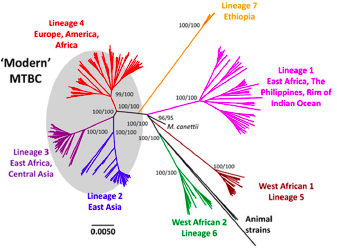
\includegraphics[scale=0.7]{worldlignee.png}
\caption{Phylogénie du génome complet de MTBC, d'après\\ \textit{Out-of-Africa migration and Neolithic coexpansion of Mycobacterium\\tuberculosis with modern humans}}
\end{figure}

% Neolithic co-expansion of MTBC and humans

Dans tous les cas, la tuberculose aurait infecté l'espèce humaine et évolué conjointement avec elle depuis 70 000 ans, mais son apparition serait antérieure à la transition démographique du Néolithique.

La base de données de tuberculose étudiée de façon probabiliste par Comas et al.\cite{comas} montre que le Néolithique a fortement contribué à l'expansion de la maladie il y a 10 000 ans grâce à l'augmentation de la densité de population et à la probabilité de co-infection avec d'autres maladies également dépendantes de la densité de population. La possibilité pour la tuberculose de muter d'une variété animale vers une variété humaine n'est en revanche pas retenue par Comas et al. En effet, l'analyse phylogénique de la tuberculose montre que les branches humaines ont divergé des branches animales avant le Néolithique.

Le Néolithique n'était pas la seule période où l'augmentation de la population fut importante, toutefois la concentration de population qui s'en est suivie a permis l'apparition, auprès de la tuberculose, de caractères fortement dépendants de la densité de population qu'elle affecte. Le Néolithique a donc marqué un tournant dans l'histoire de la tuberculose, qui a alors commencé à conjuguer les deux principaux modèles de maladie, d'une part dépendant de la densité de population et d'autre part s'apparentant à une infection chronique. En effet, le mode de transmission aérosol de la tuberculose s'est parfaitement adapté aux foules, et elle a montré à travers les âges des périodes de latence et de réactivation.

% The evolutionary history of MTBC at a regional scale
% Conclusion

Il faut donc considérer que la co-existence de la tuberculose avec l'espèce humaine depuis des milliers d'années a conduit la maladie à s'adapter aux changements du génome humain et inversement. Les prochaines études sur la tuberculose devraient donc se concentrer sur des génomes complets de la tuberculose et de l'être humain choisis en rapport à leurs associations.

En particulier, la tuberculose a dû s'adapter aux autres infections ayant touché l'espèce humaine, avec plus ou moins de succès. Dans cet ordre d'idée, une étude récente de Perry S. et al.\cite{perry1, perry2} suggère que l'infection d'un organisme par \textit{Helicobacter Pylori} pourrait protéger de la tuberculose sous sa forme active. A contrario, nous ne savons pas si la tuberculose latente pourrait protéger contre les ulcères et les cancers de l'estomac causés par \textit{Helicobacter Pylori}.

\begin{figure}
\centering
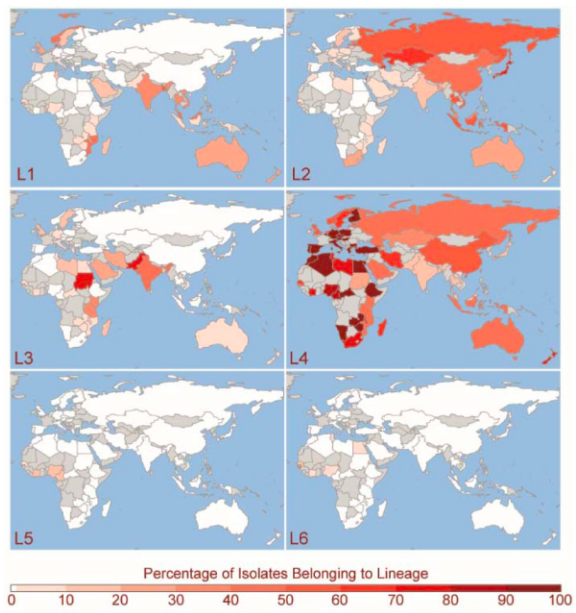
\includegraphics[scale=0.5]{world.png}
\caption{Distribution géographique des lignées 1 à 6, d'après \textit{Lineage\\ specific histories of Mycobacterium tuberculosis dispersal in Africa and Eurasia}}
\end{figure}

%  GLOBAL EXPANSION OF MTBC LINEAGE 4 =============================================

\section{Le développement de souches résistantes aux antibiotiques}

\subsection{L'expansion de la lignée 4 de \textit{M. tuberculosis}}

% global diversity of L4
% phylogeographic inference

La lignée 4 de \textit{M. tuberculosis} est la plus répandue de par le monde et pour cette raison a fait l'objet de nombreuses publications. Brynildsrud O.B. et al.\cite{brynildsrud} utilisent des méthodes d'analyse discrète et une approche bayésienne\footnote{\index{Approche bayésienne}\textbf{Approche bayésienne} : méthode probabiliste basée sur le calcul des probabilités postérieures des arbres phylogéniques par la combinaison d'une probabilité antérieure avec la fonction de vraisemblance} en phylogénie moléculaire pour obtenir de manière formelle l'évolution phylogéographique de la lignée 4 de \textit{M. tuberculosis}. Ils estiment que le plus récent ancêtre commun de la lignée 4 est apparu en Europe en 1096 après JC. Si on considère l'Europe en tant que continent au sens large, cela ne contredit pas les résultats de O'Neil M.B. et al.\cite{oneil} qui estiment l'origine de la lignée 4 autour de la méditerranée.

% Patterns of L4 migration through time

L'analyse phylogéographique de Brynildsrud O.B. suggère que les premières vagues de migration de la lignée 4 hors d'Europe se sont déroulées au début du 13ème siècle vers l'Asie du Sud-Est. Il est également possible d'établir une correspondance entre la structure des isolats\footnote{\index{Isolat}\textbf{Isolat} : fragment d'organisme qu'on a isolé à des fins d'examen histo-pathologiques ou pour être cultivé in vitro.} Vietnamiens et l'époque de l'expansion coloniale française en Indochine au 19ème siècle.

Les vagues suivantes de migration de la lignée 4 se sont dirigées vers l'Afrique de l'Ouest au 15ème siècle, puis vers Afrique de l'Est et du Sud au 17ème siècle. Les échanges continus avec le Portugal dès le 15ème siècle ont favorisé la dispersion de la maladie, ce qui a été renforcé plus tard par la colonisation française de l'Afrique de l'Ouest.  Ces échanges avec les populations européennes ont prévalu à une transmission locale de la tuberculose jusqu'au 19ème siècle. 

La transmission de la maladie en Amérique date, elle aussi, du 15ème siècle avec la colonisation du continent, mais il faudra attendre le 17ème siècle pour voir l'explosion de la maladie en Amérique du Sud. Ce retard dans l'évolution de la maladie par rapport à la branche africaine peut s'expliquer par le taux de mortalité élevé des populations aborigènes au contact des européens.

La première migration interne de la maladie en Afrique date de l'Empire Zulu au 19ème siècle et se dirigeait vers le Nord et l'Est africain.

Ainsi, Brynildsrud O.B. et al. montrent que la dispersion de la lignée 4 est essentiellement liée à l'expansion coloniale européenne en Afrique et en Amérique entre le 17ème et le 19ème siècle.

% antibiotiques

\subsection{L'adaptation de la lignée 4 pour devenir résistante aux antibiotiques}

Nous avons déjà vu que la tuberculose a su s'adapter à l'évolution géographique de l'humanité en suivant les différentes migrations humaines pour créer de nouvelles lignées ou de nouvelles souches. Il apparaît que la tuberculose est également capable de suivre l'évolution médicale de l'humanité. L'étude de Brynildsrud O.B. et al.\cite{brynildsrud} constate chez \textit{M. tuberculosis} l'émergence croissante d'une résistance à de multiples antibiotiques entre 1960 et 2000 au travers de la phylogénie de la lignée 4.

Des mutations spontanées dans le génome de la tuberculose peuvent altérer les protéines qui sont la cible des médicaments, ce qui rend les bactéries résistantes à ces médicaments. Prenons comme exemple une mutation du gène rpoB de \textit{M. tuberculosis}, qui code pour la sous-unité $\beta$\footnote{\index{Sous-unité $\beta$}\textbf{Sous-unité $\beta$} : élément de l'ARN polymérase des bactéries qui est composé de la structure suivante $\alpha_2 \beta \beta' \omega$} de l'ARN polymérase\footnote{\index{ARN polymérase}\textbf{ARN polymérase} : complexe enzymatique responsable de la synthèse de l'ARN à partir d'ADN.} de la bactérie. Dans la tuberculose non résistante, la rifampicine se lie à cette sous-unité $\beta$ et perturbe l'élongation de la transcription de l'ARN. La mutation dans le gène rpoB modifie la séquence des acides aminés et donc de la sous-unité $\beta$. Dans ce cas, la rifampicine ne peut plus se lier à la sous-unité $\beta$ de l'ARN et empêcher la transcription. La bactérie est devenue résistante. C'est bien le cas de la tuberculose, qui est considérée aujourd'hui comme une maladie résistante aux antibiotiques. 

Une souche de \textit{M. tuberculosis} est appelée MDR-TB \textit{Multi-Drug-Resistant Tuberculosis} si elle est résistante au deux anti-tuberculeux de première intention les plus puissants, l'isoniazide et le rifampicine. Dans ce cas, certaines régions du génome de \textit{M. tuberculosis} sont impliquées dans la résistance à plus d'un médicament. La découverte de nouvelles cibles moléculaires s'avère essentielle pour lutter contre ce développement de la résistance chez \textit{M. tuberculosis}. Une souche de \textit{M. tuberculosis} est appelée XDR-TB si elle est de surcroît résistante aux anti-tuberculeux de seconde intention tels que le fluoroquinolone et l'aminoglycoside.

\begin{figure}[h!]
\centering
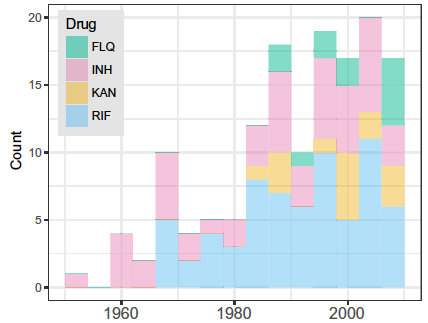
\includegraphics[scale=0.6]{amr.png}
\caption{Transmission de la résistance ces dernières années à l'échelle mondiale, d'après\\ \textit{Global expansion of Mycobacterium tuberculosis lineage 4 shaped by colonial migration and local\\ adaptation}. FLQ=fluoroquinolone, INH=isoniazide, KAN=aminoglycoside, RIF=rifampicine}
\end{figure}

Les causes de la résistance de \textit{M. tuberculosis} aux antibiotiques sont multiples, mais il s'agit principalement de l'utilisation inappropriée ou incorrecte d'antibiotiques, et de l'interruption précoce des traitements. Dans ce cas, les souches résistantes se transmettent génétiquement de générations en générations. Toutefois, ces souches résistantes de \textit{M. tuberculosis} peuvent aussi se transmettre directement à une personne saine, qui dans ce cas, se retrouve infectée avec une souche MDR-TB sans avoir pris de traitement inapproprié contre la tuberculose.

Brynildsrud O.B. et al. étudient également le gène lldD2 impliqué dans la réplication de \textit{M. tuberculosis} au sein des macrophages\footnote{\index{Macrophage}\textbf{Macrophage} : cellule appartenant aux globules blancs qui infiltre les tissus et est capable de phagocytose.} humains. Ils identifient au niveau des codons 3 et 253 la présence de nombreux promoteurs\footnote{\index{Promoteur}\textbf{Promoteur} : région de l'ADN située à proximité d'un gène et indispensable à la transcription de l'ADN.} et mutations non-synonymes qui ont évolué indépendamment.

Une recherche au sein d'une base de données recouvrant les lignées 1 à 6 a révélé que la mutation du codon 3 a émergé indépendamment dans les lignées 1, 2 et 4, alors que la mutation du codon 253 est apparue à plusieurs reprises dans la lignée 4 et est présente dans pratiquement tous les isolats de la lignée 2. Brynildsrud O.B. et al. constatent que les mutations de lldD2 ont commencé à apparaître bien avant l'utilisation des antibiotiques sur tous les continents. Ceci suppose une adaptation locale de \textit{M. tuberculosis} à de profonds changements chez l'hôte humain, qui s'est opérée en parallèle sur les différents continents. Par ailleurs, les souches hébergeant des mutations du promoteur lldD2 présentent un avantage significatif en terme de transmissibilité.

Il ne fait aucun doute que des souches MDR-TB peuvent traverser les frontières, comme cela a déjà été observé avec la lignée 2 entre l'Europe de l'Est et l'Europe de l'Ouest. Toutefois, le jeune âge relatif des souches résistantes pourrait expliquer le manque de migrations observées de ces souches. Brynildsrud O.B. et al. démontrent que, d'un point de vue mondial, la migration humaine a joué un rôle négligeable dans l'élaboration des modèles de résistance aux antimicrobiens. En effet, la migration des souches résistantes s'est avérée marginale. Il s'agit plutôt d'un phénomène local. La restriction géographique de souches résistantes suggère même de lutter contre ce type de mutation de \textit{M. tuberculosis} de façon nationale plutôt que de recourir à une politique globale de traitement antibiotique.

% SPOLPRED ==========================================================

\section{Le locus CRISPR-Cas}

\subsection{Quelques caractéristiques du génome de \textit{M. tuberculosis}}

La souche H37Rv de \textit{M. tuberculosis} est la souche de tuberculose la plus étudiée en laboratoire, depuis sa découverte en 1905. Elle sert aujourd'hui de référence pour le séquençage et l'annotation du génome de \textit{M. tuberculosis}. Constitué d'environ 4 millions de paires de base et 3959 gènes, ce génome se caractérise par un taux élevé de guanine G et de cytosine C (65,6\%), et un codon GTG qui sert de codon d'initiation dans 35\% des gènes. 

Parmi les marqueurs génétiques utilisés pour des études phylogéniques ou d'épidémiologie moléculaire, on retrouve les SNPs, les loci CRISPR, les MIRU\footnote{\index{Marqueur MIRU}\textbf{Marqueur MIRU Mycobacterial Interspaced Repetitive Units} : séquences nucléotidiques courtes répétitives en tandem entrecoupées de mycobactéries. La méthode MIRU actuellement utilisée sur \textit{M. tuberculosis} est composée de 12 loci MIRU différents. Un mirutype est un modèle à 12 chiffres représentant le nombre de répétitions de chacun de ces 12 loci spécifiques.}, et les VNTR\footnote{\index{Marqueur VNTR}\textbf{Marqueur VNTR Variable Number of Tandem DNA Repeats} : séquences nucléotidiques courtes en tandem à nombre variable. Cinq répétitions en tandem exactes ( locus ETR) sont utilisées pour l'analyse VNTR du complexe \textit{M. tuberculosis}.}. L'association des résultats obtenus par ces marqueurs génère un profil allélique\footnote{\index{Allèle}\textbf{Allèle} : version variable d'un même gène.} utile pour l'étude du complexe \textit{M. tuberculosis}. La base de données mondiale de marqueurs moléculaires de la tuberculose SITVIT\footnote{\index{Base de données SITVIT}\textbf{Base de données SITVIT} : base de données de l'Institut Pasteur de Guadeloupe consultable en ligne \url{http://www.pasteur-guadeloupe.fr:8081/SITVIT_ONLINE/query}, permettant n'analyser des data liées au MTBC. Elle comprend les spoligotypes de \textit{M. tuberculosis}, ainsi que les marqueurs utilisés pour les détecter MIRU12, VNTR, SIT, MIT, VIT, les différentes branches de MTBC, les pays d'origine et l'année de découverte.} présentée par Demay C. et al.\cite{demay} contient les génotypes de \textit{M. tuberculosis} obtenus à partir des marqueurs moléculaires MIRU et VNTR.

% Le locus CRISPR Cas

\subsection{Description du locus CRISPR-Cas}

\begin{figure}[h!]
\centering
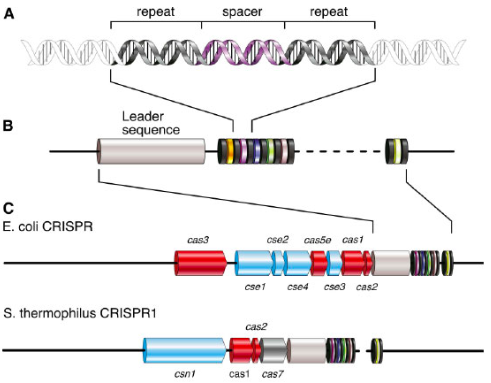
\includegraphics[scale=0.6]{crispr.png}
\caption{Structure du locus CRISPR-Cas, d'après\\ \url{https://www.sinobiological.com/crispr-locus.html}}
\end{figure}

Le locus CRISPR \textit{Clustered Regularly Interspaced Short Palindromic Repeats} est une famille de séquences répétées (DR pour \textit{Direct Repeat}) dans l'ADN formant un palindrome, qui se trouve à l'état naturel chez 40\% des bactéries (dont le \textit{M. tuberculosis}) et la plupart des archées. CRISPR est héritable par transmission aux cellules filles et se conserve donc pour une même espèce. Chez \textit{M. tuberculosis}, chaque série de répétitions contient 36 bp\footnote{\textbf{bp} : une paire de base.}; les répétitions étant régulièrement espacées par des espaceurs de 34 à 41 bp. A l'heure actuelle, 104 espaceurs ont été identifiés dans toutes les souches de \textit{M. tuberculosis}. Les loci CRISPR sont généralement adjacents aux gènes Cas, dont ils sont séparés par une séquence de 300 à 500 bp, appelée leader qui contrôle à la fois l'acquisition de l'ADN viral par les espaceurs et la fabrication des protéines. Les gènes Cas produisent des protéines aux fonctionnalités multiples et notamment les enzymes\footnote{\index{Enzyme de restriction}\textbf{Enzyme de restriction} : protéine capable de couper un fragment d'ADN au niveau d'une séquence de nucléotides caractéristique appelée site de restriction. Chaque enzyme de restriction reconnaît ainsi un site spécifique.} capables de couper l'ADN en vue de sa réparation.

Ces séquences CRISPR incorporent dans les espaceurs des fragments d'ADN de bactériophages qui ont déjà infecté la bactérie, et sont stockés pour détecter et détruire l'ADN de bactériophages similaires en cas de nouvelle infection. Par conséquent, CRISPR-Cas est un système immunitaire naturel utilisé par les bactéries pour se protéger des infections virales. 

% Fonctionnement du système CRISPR-Cas 

\subsection{Fonctionnement du système CRISPR-Cas}

Les systèmes CRISPR-Cas sont de trois types et utilisent les différents gènes Cas pour intégrer des fragments de gènes étrangers dans les espaceurs de CRISPR. Par exemple, dans le cas d'une bactérie qui détecte la présence d'ADN ou d'ARN d'un virus, elle produit une enzyme nucléase appelée Cas9 capable de couper l'ADN viral, puis une séquence d'ARN CRISPR notée crARN correspondant à celle de l'ADN du virus et servant de guide ARN, et finalement une séquence d'ARN traceur notée trARN. Lorsque trARN trouve sa cible parmi le génome du virus, Cas9 sectionne l'ADN viral puis en incorpore un fragment dans un espaceur du génome de la bactérie, conservant ainsi en mémoire une trace de ce virus en vue d'une éventuelle infection future. Les espaceurs servent donc de banque de mémoire en conservant l'ADN des virus qui ont attaqué la bactérie. Cette fonctionnalité va être exploitée de différentes manières par les biologistes.

La technologie CRISPR-Cas9, s'inspirant du système du même nom, a d'abord été utilisée pour typer les souches bactériennes, suivant une technique appelée spoligotypage. CRISPR-Cas9 est actuellement principalement employé comme ciseau moléculaire afin d'éditer le génome et d'introduire localement des modifications génétiques.

% Spoligotyping

\section{Le spoligotypage}

La région DR du locus CRISPR-Cas présente un niveau de polymorphisme suffisant pour pouvoir classer phylogéographiquement les souches de \textit{M. tuberculosis}. Le polymorphisme entre les différentes souches résulte des variations et de l'identité des espaceurs. C'est ce polymorphisme qui est exploité en 1997 par Kamerbeek et al. et expliqué dans \cite{kamerbeek} comme technique de génotypage spécifique de \textit{M. tuberculosis}. Le \textit{Spacer Oligonucleotide Typing}, repose sur la détection de séquences répétitives trouvées entre les gènes d'un agent infectieux au sein d'un locus CRISPR-Cas. Pour ce faire, la région DR d'un isolat à tester subit un traitement par amplification PCR\footnote{\index{PCR}\textbf{PCR Polymerase Chain Reaction} : méthode de réaction en chaîne utilisant un polymère pour dupliquer en grand nombre une séquence d'ADN spécifique. La méthode PCR repose sur le cycle thermique, qui expose les séquences à des cycles répétés de chauffage et de refroidissement pour permettre différentes réactions dépendantes de la température comme la fusion de l'ADN et la réplication de l'ADN par les enzymes. La méthode PCR utilise deux agents principaux : les polymères d'ADN i.e. des macromolécules répétant un même motif structural d'ADN et les amorces de séquençage.} ou celui d'une puce à ADN\footnote{\index{Puce à ADN}\textbf{Puce à ADN} : ensemble de molécules d'ADN fixées sur une petite surface solide permettant de mesurer le niveau d'expression d'un grand nombre de gènes simultanément, ou de déterminer le génotype de plusieurs régions d'un génome.}, pour dévoiler un motif de taches correspondant aux espaceurs. 

\begin{figure}[h!]
\centering
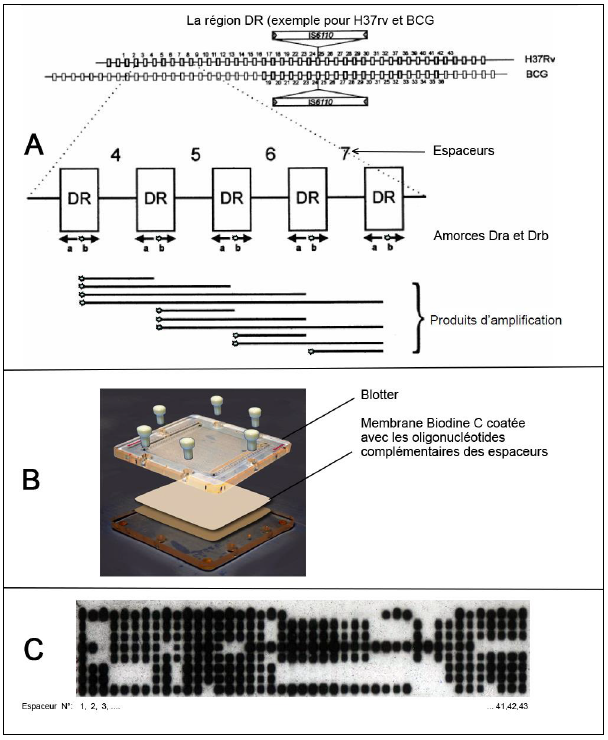
\includegraphics[scale=0.4]{spoligo.png}
\caption{Les différentes étapes du spoligotypage d'après \textit{Etudes descriptive, épidémiologique,\\ moléculaire et spatiale des souches Mycobacterium tuberculosis circulant à Antananarivo, Madagascar}}
\end{figure}

La comparaison de ces motifs permet la différentiation des souches. Quarante-trois espaceurs les plus polymorphes ont été utilisés pour le typage des mycobactéries suivant Kamerbeek et al. La classification classique de MTBC utilise donc un groupe de 43 bits représentant la présence ou l'absence d'espaceurs dans le locus CRISPR, qu'on appelle spoligotype. Des études pour augmenter le niveau de discrimination du spoligotypage ont été faites en 2010 utilisant 68 espaceurs. A l'heure actuelle l'équipe AND de l'université de Franche Comté utilise 98 espaceurs pour ce génotypage.

\begin{figure}[h!]
\centering
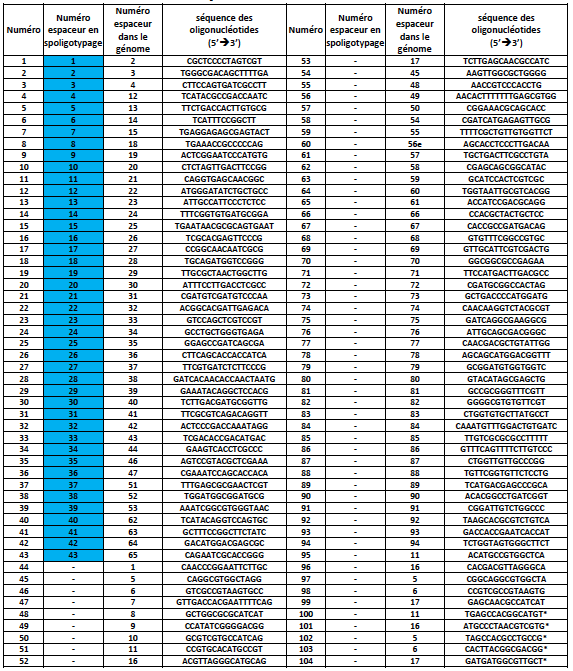
\includegraphics[scale=0.7]{spacer.png}
\caption{Espaceurs connus chez MTBC, d'après \textit{Etudes descriptive, épidémiologique, moléculaire\\ et spatiale des souches Mycobacterium tuberculosis circulant à Antananarivo, Madagascar}}
\end{figure}

La technique ne nécessite pas une importante quantité d'ADN car elle est basée sur une amplification de la région DR par PCR. Les spoligotypes ainsi obtenus peuvent être partagées entre laboratoires et corroborent les résultats recueillis à partir d'autres marqueurs génétiques. Ces données numériques permettent de bien différencier les souches de \textit{M. tuberculosis} et sont de moindre coût comparativement à d'autres méthodes. Cependant, le spoligotypage éprouve des difficultés à bien différencier les souches au sein de grandes familles de \textit{M. tuberculosis} telles que la lignée 2 par exemple.

Jusqu'à présent, le spoligotypage a permis de fournir une image globale de la diversité des souches de \textit{M. tuberculosis}.

Une nouvelle technologie permettant de combiner le spoligotypage avec des tests moléculaires de sensibilité aux anti-tuberculeux, appelée spoligoriftypage, a été développée pour aboutir à la version TB-SPRINT qui a été décrite en 2013 par Gomgnimbou et al. dans leur article \cite{gomgnimbou}. Elle consiste au typage tuberculose-spoligo-rifampicine-isoniazide fonctionnant sur des systèmes à base de microbilles, à partir notamment de 43 espaceurs, 11 SNPs présents sur rpoB aux positions 516, 526 et 531. Cette nouvelle génération de spoligotypage fournit donc, en plus des données classiques de génotypage, une prédiction basée sur la mutation des profils de résistance aux médicaments.

% Normalisation

\subsection{Vers une normalisation des spoligotypes}

Au début du spoligotypage, il n'existait pas de norme pour décrire les motifs formés par les espaceurs ou simplement les numéroter. Chaque laboratoire utilisait son propre système de numérotation accompagné d'un schéma descriptif du motif. Ce manque de normalisation entravait les possibilités de comparaison des résultats obtenus et le développement d'une vision mondiale de l'évolution de \textit{M. tuberculosis}. Une méthode standardisée de description des spoligotypes a été proposée en 2001 par Dale JW dans son article \cite{dale}. 

Tout d'abord, une base de données centralisée regroupant tous les motifs connus et de leurs numérotations associées existe au RIVM Rijksinstituut voor Volksgezondheid en Milieuhygiene, Bilthoven, Netherlands. Elle peut être consultée au \url{http://www.caontb.rivm.nl}. A partir de 2001, les nouveaux motifs doivent prendre un unique format de numérotation pour être répertoriés dans cette base de données. Toutefois, cela nécessite l'interrogation systématique de la base de données et la comparaison avec les éléments déjà existants pour chaque nouveau spoligotype. Pour éviter cette perte de temps, de nombreux laboratoires utilisent des systèmes rationnels avec des codes descriptifs assignés à chaque isolat. 

Dale JW et al.\cite{dale} proposent d'utiliser exclusivement un système rationnel octal ou hexadécimal, sachant qu'il est aisé de passer de l'un à l'autre et qu'il est également facile de retrouver l'état initial binaire. Ainsi, les motifs de spoligotype comprenant 43 bits seraient réduits dans le système octal en 14 groupes de 3 bits auquel s'ajouterait un unique bit, ce qui donnerait finalement un ensemble de 15 chiffres en écriture octale. En ce qui concerne le système hexadécimal, les motifs de 43 bits seraient réduits en 6 groupes de 8 bits avec un dernier groupe ne comprenant que 3 bits, soit 6 groupes de 2 chiffres hexadécimaux. Notons qu'un bit symbolise dans ce cas la présence ou l'absence d'une espaceur dans le locus étudié.

\begin{figure}[h!]
\centering
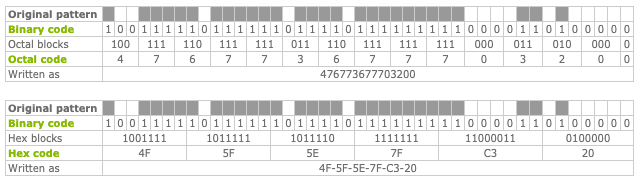
\includegraphics[scale=0.6]{hexa.png}
\caption{Exemple de système rationnel octal et hexadécimal, d'après\\ \url{https://www.mbovis.org/spoligotype-nomenclature.php}}
\end{figure}

Le site Mbovis.org, \url{https://www.mbovis.org/database.php}, bien que dédié aux souches animales de MTBC, fournit une application pratique permettant de transformer rapidement les spoligotypes binaires en système octal ou hexadécimal.

% Spolpred et SpoTyping

\subsection{Quel outil informatique pour le spoligotypage ?}

Les technologies PCR de génotypage utilisent toujours différents marqueurs tels que les SNPs pour obtenir en laboratoire des résultats fiables. Des logiciels informatiques de prédiction du génotype ont également fait leur apparition pour optimiser les coûts et le gain de temps. Ils offrent un outil de comparaison des résultats obtenus expérimentalement et in silico.

SpolPred est un logiciel de prédiction rapide et précis des spoligotypes de \textit{M. tuberculosis} à partir de séquences génomiques courtes appelées reads\footnote{\index{Reads}\textbf{Reads} : mélange de courtes séquences oligonocléotidiques de 20 à 200 bp générées par des séquenceurs}. Cet outil développé par Coll F. et al. fonctionne efficacement avec des reads provenant de plateformes telles que Illumina GAII ou HiSeq. SpolPred utilise des fichiers de séquences de reads simples ou par paires au format FASTQ, afin de produire une prédiction de spoligotype au format octal, qui est ensuite comparée au spoligotype correspondant dans la base SITVIT.

\begin{figure}[h!]
\centering
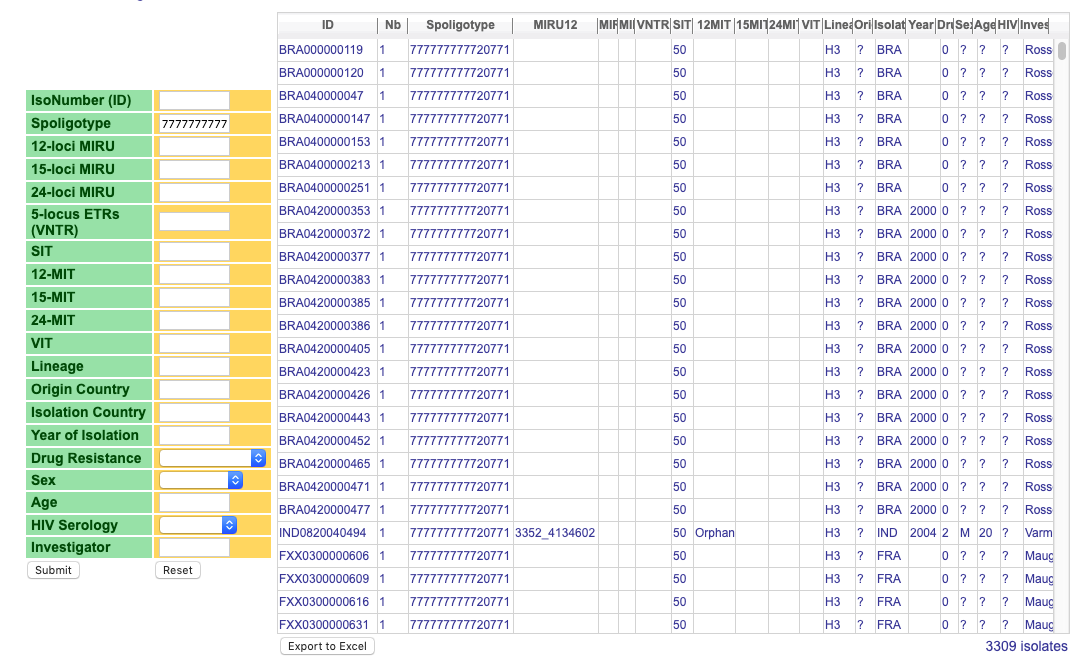
\includegraphics[scale=0.44]{spol.png}
\caption{Exemple de recherche effectuée sur SITVIT2 à partir du spoligotype 777777777720771 dont le résultat est exploitable au format Excel}
\end{figure}

Dans leur étude \cite{coll}, Coll F. et al. montrent en 2012 l'utilité de SpolPred en comparant les spoligotypes obtenus par le logiciel avec les résultats de laboratoire. Ils dévoilent ainsi les limites de la méthode expérimentale qui a répertorié cinq faux spoligotypes, alors que SpolPred a su éviter ces erreurs de classification du génotype. Par ailleurs, il apparaît que SpolPred offre plus de rapidité avec des résultats pratiquement identiques à ceux obtenus avec la méthode bio-informatique par assemblage. Cette dernière, développée en 2008 à l'aide du logiciel Velvet, consiste à fusionner des fragments d'ADN issus d'une plus longue séquence afin d'en reconstruire la séquence originale.

Toutefois, d'après l'étude de Xia et al.\cite{xia}, la précision de SpolPred est fortement réduite lorsque les reads n'ont pas une taille uniforme, comme par exemple lorsqu'ils proviennent de séquençages Ion Torrent ou de la plateforme de diagnostique clinique Illumina MiSeq. Ainsi, lorsque les reads ne sont pas uniformes, la précision des résultats dépend fortement de leurs tailles et donc du choix initial fait par l'opérateur. Par ailleurs, SpolPred demande à l'utilisateur de spécifier la direction de lecture des reads, et le logiciel n'utilise donc qu'une partie des informations fournies par les reads.

Une problématique de SpolPred en 2020 est que le logiciel n'est plus disponible au téléchargement en ligne. En effet, une visite sur le site officiel \url{http://www.pathogenseq.org/spolpred}, fourni comme référence dans le document \cite{coll} de Coll F. et al., montre que le nom du domaine est à vendre. Preston M., qui a fait partie de l'équipe de recherche de Coll F. pour le développement de SpolPred, a bien créé un site proposant le téléchargement du logiciel \url{https://www.mybiosoftware.com/spolpred-predict-the-spoligotype-from-raw-sequence-reads.html}, mais le lien est inactif en janvier 2020.

Une alternative à SpolPred est SpoTyping présenté en 2016 dans l'article \cite{xia} de Xia et al. comme étant 20 à 40 fois plus rapide que SpolPred pour prédire avec précision des spoligotypes de \textit{M. tuberculosis} à partir de reads de taille uniforme ou variable. Par ailleurs, SpoTyping lit chaque read dans les deux directions en exploitant complètement les informations fournies. SpoTyping réduit la durée des recherches en intégrant l'algorithme BLAST\footnote{\index{BLAST}\textbf{BLAST Basic Local Alignment Search Tool} : logiciel basé sur l'algorithme du même nom qui détecte des régions similaires entre plusieurs séquences biologiques. Le programme compare les séquences de nucléotides aux séquences contenues dans la base de données BLAST pour fournir des résultats statistiquement significatifs.} dans ses calculs. Il compare les isolats testés avec ceux ayant le même spoligotype dans la base de données mondiale SITVIT, qui regroupe les données épidémiologiques\footnote{\index{Epidémiologie}\textbf{Epidémiologie} : discipline scientifique qui étudie les problèmes de santé dans les populations humaines, leur fréquence, leur géographie ainsi que les facteurs influents.} associées à des isolats de même spoligotype.

L'intérêt d'un outil tel que SpolPred ou Spotyping est qu'il est capable de combiner le spoligotypage avec d'autres méthodes telles que MIRU (unités répétitives entrecoupées de mycobactéries) et VNTR nombre variable de répétitions d'ADN en tandem) en utilisant la base de données SITVIT.

SpoTyping utilise des fichiers de séquences de reads simples ou par paires au format FASTQ et des fichiers de séquences complètes de génomes ou de contigs\footnote{\index{Contig}\textbf{Contig} : séquence génomique continue et ordonnée, générée par l'assemblage des clones d'une bibliothèque génomique qui se chevauchent.} assemblés au format FASTA. Les séquences de reads sont regroupées en une unique séquence continue au format FASTA pour être ensuite soumise à l'algorithme BLAST qui détecte les régions similaires. Finalement la base de données SITVIT permet d'identifier les isolats ayant le même spoligotype. SpoTyping est limité à une lecture de 250 Mbp au sein des séquences de reads testées, lors de l'utilisation du swift mode qui accélère le temps de traitement.

SpoTyping propose un rapport statistique permettant de résumer le rapprochement avec les spoligotypes trouvés dans la base de données SITVIT, ainsi qu'une estimation du nombre de correspondances positives pour chaque espaceur.

\begin{figure}[h!]
\centering
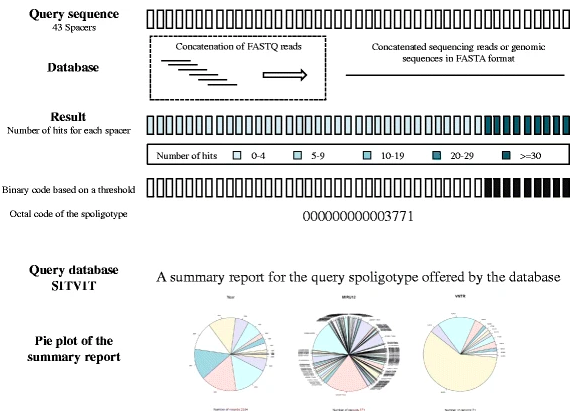
\includegraphics[scale=0.65]{spotyping.png}
\caption{Exemple de fonctionnement de SpoTyping, d'après \textit{SpoTyping:\\ fast and accurate in silico Mycobacterium spoligotyping from sequence reads}}
\end{figure}

D'après le repository \url{https://github.com/xiaeryu/SpoTyping-v2.0/blob/master/SpoTyping-v2.0-commandLine/SpoTyping-README.pdf}, les spécifications techniques de SpoTyping sont les suivantes :\\
- SpoTyping peut s'exécuter sur les principaux systèmes d'exploitation, contrairement à SpolPred qui utilise exclusivement Linux. Il se présente à la fois sous forme de script et sous forme d'application avec une interface graphique.\\
- SpoTyping est un logiciel open-source qui peut se télécharger gratuitement à l'adresse \url{https://github.com/xiaeryu/SpoTyping-v2.0}. SpoTyping nécessite l'utilisation de Python2.7 et BLAST.\\
- il est recommandé d'utiliser le swift mode paramétré par défaut si le débit de séquençage\footnote{\index{Séquençage du génome}\textbf{Séquençage du génome} : consiste, par des méthodes chimiques ou de biologie moléculaire, à déterminer l'ordre des nucléotides de l'ADN.} est inférieur à 135 Mbp. Pour les débits de séquençage inférieurs à 135 Mbp ou supérieurs à 1260 Mbp, les seuils doivent être réglés entre 0.018 et 0.1486 fois la profondeur de lecture estimée pour les hits sans erreur, et entre 0.018 et 0.1488 fois la profondeur de lecture estimée pour les hits tolérant une erreur. Notons que la profondeur de lecture est définie par le débit de séquençage divisé par 4 500 0000 qui correspond à l'estimation de la longueur d'un génome de \textit{M. tuberculosis}.

Le fichier obtenu propose une prédiction de spoligotype au format de code binaire et octal. Le fichier log obtenu contient le nombre de correspondances positives des résultats de BLAST pour chaque séquence d'espaceurs. Le fichier xls Excel obtenu fournit le résultat de la recherche de spoligotype auprès de la base de données SITVIT2\footnote{\index{Base de données SITVIT2}\textbf{Base de données SITVIT2} : mise à jour de la base de données SITVIT, consultable en ligne \url{http://www.pasteur-guadeloupe.fr:8081/SITVIT2/index.jsp}}.

L'étude de Iwai H. et al.\cite{iwai} envisage une autre possibilité de travail et montre l'intérêt d'une analyse de \textit{M. tuberculosis} à l'aide de serveurs, appelée CASTB, et notamment le spoligotypage. Le Webserver fournit une vue complète des données, mais les performances de chaque outil utilisé ne sont pas décrites dans l'article. Il est probable que le spoligotypage prenne plus de temps en passant par un serveur suite au problème de disponibilité des données et aux lenteurs de téléchargement de ces données. Il semblerait que SpoTyping, de par sa configuration locale, puisse fournir un résultat en une minute.

% Comparaison de spoligotypes

\subsection{Comparaison de spoligotypes}

Une fois les spoligotypes de différentes lignées obtenus, il est nécessaire de les comparer pour chercher à faire ressortir les points communs ou certains traits pouvant être liés à une mutation particulière. Il existe à l'heure actuelle un premier outil en ligne de comparaison du nom de SpolSimilaritySearch, accessible à l'adresse \url{http://www.pasteur-guadeloupe.fr:8081/SpolSimilaritySearch/index.jsp}, et présenté par Couvin D. et al.\cite{couvin}. SpolSimilaritySearch incorpore un algorithme de recherche de similitudes entre spoligotypes dans la base de données SITVIT2. Cet outil permet d'analyser les modèles de propagation et d'évolution de \textit{M. tuberculosis} en comparant des modèles de spoligotypes similaires, de distinguer les modèles répandus, confinés ou spécifiques, d'identifier les modèles ayant de grands blocs supprimés ou encore de fournir les modèles de distribution par pays pour chaque spoligotype interrogé.

Par exemple, si on sélectionne le spoligotype 777777777720771 appartenant à la lignée H3, et qu'on interroge la base SpolSimilaritySearch, on obtient les rapprochements suivants :

\begin{figure}[h!]
\centering
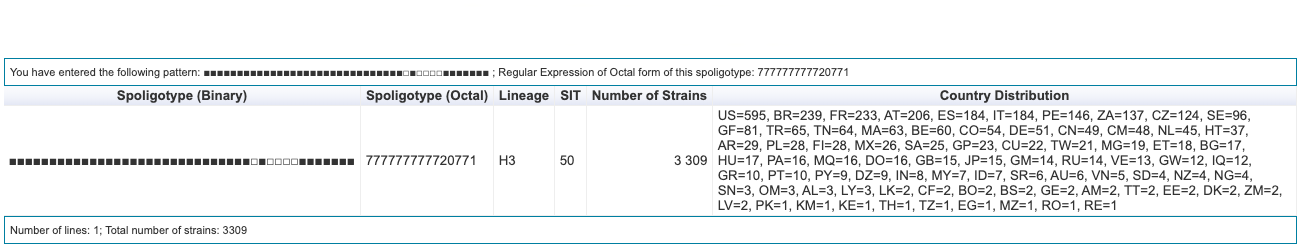
\includegraphics[scale=0.37]{spolsimilarity.png}
\caption{Recherche effectuée sur le site de SpolSimilaritySearch}
\end{figure}

Cet outil pourrait donc s'avérer utile pour commencer à chercher des liens entre les sept lignées de \textit{M. tuberculosis} et les spoligotypes de différentes souches.
Un tableau comparatif de différents spoligotypes en fonction des lignées de \textit{M. tuberculosis} pourrait ressembler à celui de la figure 11.

\begin{figure}[h!]
\centering
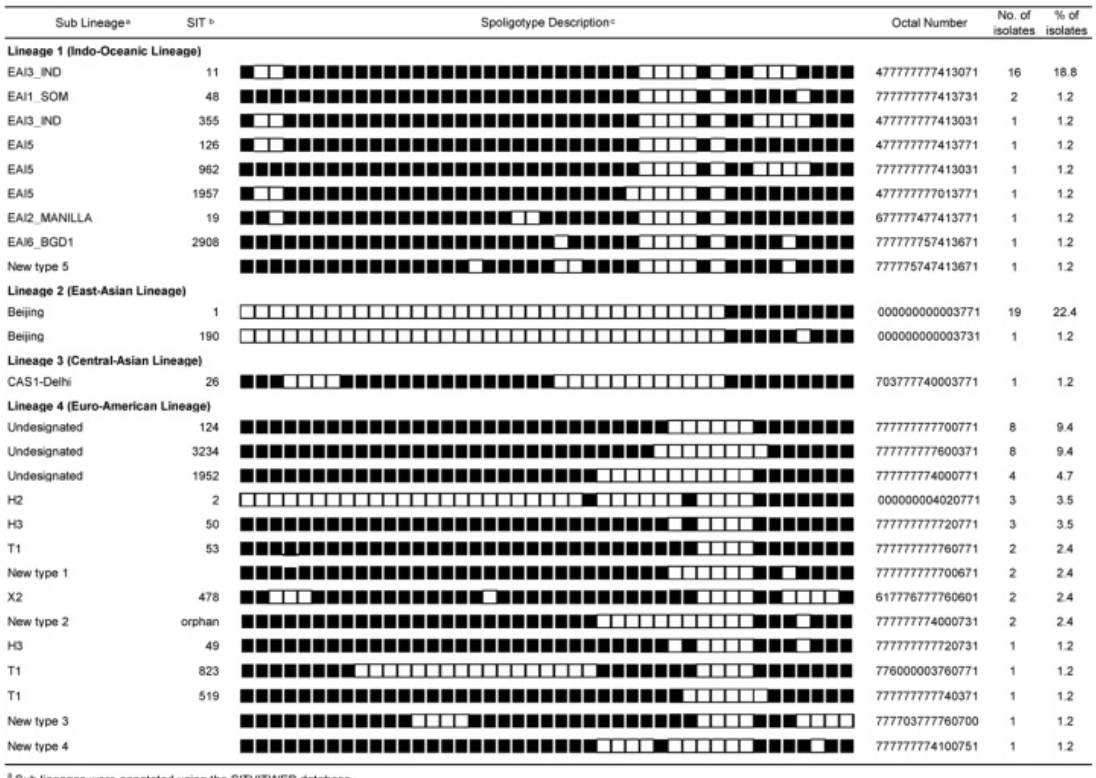
\includegraphics[scale=0.4]{comparaison.png}
\caption{Exemple comparatif de 26 spoligotypes correspondant à 4 lignées différentes de \textit{M. tuberculosis}, d'après \textit{Insight into genetic diversity of Mycobacterium tuberculosis in Kandy, Sri Lanka reveals predominance of the Euro-American lineage}}
\end{figure}
	


% LA NOTION DE PACKAGE ---------------------------
\chapter{La notion de package}

Le packaging ou distribution de programmes pose traditionnellement plus de problèmes en Python que dans d'autres langages. En effet, les standards ont évolué de façon concurrentielle plutôt que collaborative. Par ailleurs, la documentation sur Internet est parfois obsolète et entraîne de nombreuses incompréhensions. Nous verrons que l'arrivée de l'outil \textit{Poetry} a grandement facilité la création et la gestion des packages. Des sites tels que \url{https://realpython.com/python-modules-packages/}, \url{https://realpython.com/pypi-publish-python-package/}, ~\url{https://python-poetry.org/} ou \\ \url{https://packaging.python.org/overview/} ont également contribué à rendre accessible le packaging au grand public.





% COMPOSITION D'UN PACKAGE STANDARD ------------------
\section{Composition d'un package standard}

Un \index{package} permet de fournir une structure hiérarchisée du programme, pour en faciliter la compréhension et l'utilisation. Il s'agit en fait d'un ensemble de modules Python, de modules écrits en C, de métadonnées et de bases de données.

Un package standard comporte traditionnellement un fichier \textbf{\_\_init\_\_.py} dans chaque répertoire, même si ce répertoire est vide. En particulier, le répertoire racine du package contient un fichier \textbf{\_\_init\_\_.py} qui peut définir la version du projet et le nom des modules à importer. Il est toutefois acceptable et parfois même recommandé de conserver ce fichier \textbf{\_\_init\_\_.py} vide.

Par ailleurs, dans le cas d'un package exécutable, il est essentiel que celui-ci contienne un module de lancement du programme appelé  \textbf{\_\_main\_\_.py}.

Du point de vue du développeur, il est nécessaire de rajouter des fichiers permettant la construction du package et comportant les métadonnées du package. Ainsi, les fichiers \textbf{setup.py}, \textbf{requirements.txt}, \textbf{LICENSE},  \textbf{README.md} et \textbf{MANIFEST.in} sont nécessaires.  
\begin{itemize}
\item \textbf{setup.py} est le script de construction et configuration destiné au \textit{setuptools}. Il définit notamment le nom et la version du package, ainsi que les fichiers qu'il contient. Il sert également d'interface en ligne de commande relative aux différentes fonctionnalités du package. \textbf{setup.cfg} est un fichier d'initialisation qui contient les options par défaut des commandes du \textbf{setup.py}.
\item \textbf{requirements.txt} permet l'installation des dépendances à l'aide d'un unique fichier contenant un module à installer par ligne. Il nécessite l'instruction 
\texttt{pip install -r requirements.txt}
pour commencer ces installations.
\item \textbf{LICENSE} définit les termes légaux de la distribution. De nombreux pays n'autorisent pas l'utilisation ou la distribution d'un package qui ne dispose pas de licence.
\item \textbf{README.md} décrit l'objectif du package, son installation, la nature de ses dépendances et les principales fonctionnalités.
\item \textbf{MANIFEST.in} permet d'inclure dans le package certains fichiers qui ne sont pas automatiquement intégrés. 
\end{itemize}

L'ensemble des modules nécessaires au fonctionnement du package sont regroupés dans un répertoire portant le même nom que celui du package. C'est ce répertoire qui sera archivé et distribué en mettant à jour le numéro de version dans les fichiers \textbf{\_\_init\_\_.py} et \textbf{setup.py}. Si au lieu de stocker les modules dans ce répertoire, on les place à la racine du package, alors la distribution du package se construit à vide, l'installation à partir de PyPI fonctionne quand même, mais l'exécution du package ne produit rien.

Par ailleurs, les packages construits pour des systèmes Linux et macOS nécessitent l'incorporation de fichiers \textbf{build.sh} et \textbf{meta.yaml} alors que les packages construits pour les systèmes Windows nécessitent l'incorporation des fichiers \textbf{bld.bat} et \textbf{meta.yaml}.

Il faut également rajouter l'archive et la distribution compilée en vue de publier le package.

Ainsi, lorsqu'un utilisateur télécharge l'archive d'un package à partir de PyPI, celui-ci présente la structure suivante 

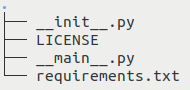
\includegraphics[width=5.5cm]{mon_package1.png}

Nous ne rentrerons pas plus dans le détail de la création d'un package standard, car nous avons choisi de construire CRISPRbuilder\_TB avec l'outil \textit{Poetry}. En effet, nous avons commencé par construire manuellement notre package en incorporant les fichiers ci-dessus un par un, jusqu'à ce que les discordances rencontrées entre les contenus de ces fichiers orientent nos recherches vers un outil permettant l'automatisation du processus et la gestion des incompatibilités.






% COMPOSITION D'UN PACKAGE SOUS POETRY ----------------------
\section{Composition d'un package sous poetry}

Avec la PEP-518\footnote{\index{PEP-518}\textbf{PEP-518:} specifying minimum build system requirements for Python projects}, le PyPA\footnote{\index{PyPA}\textbf{PyPA:} Python Packaging Authority} a proposé un nouveau standard au format \textit{.toml} pour regrouper les métadonnées d'un package et le construire à l'aide de \textit{Poetry}. 

Du point de vue du développeur, un package, appelé \textit{mon\_package}, présente la structure suivante lorsqu'il est construit avec \textit{Poetry} :

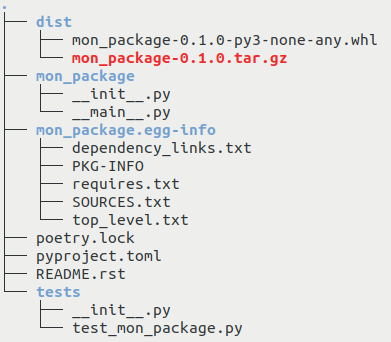
\includegraphics[width=9cm]{mon_package_poetry_complet.png}

\begin{itemize}
\item le répertoire \textbf{dist} contient l'archive des sources du package \textbf{mon\_package-0.1.0.tar.gz} (ici la version 0.1.0), construite en compressant le répertoire \textbf{mon\_package}. Il contient également la distribution compilée \textbf{mon\_package-0.1.0-py3-none-any.whl} permettant d'installer l'archive sur le système de l'utilisateur et de rendre le package exécutable. 
\item la création du répertoire \textbf{mon\_package}, portant le même nom que celui du package, est automatique avec \textit{Poetry}, de même que celle des fichiers \textbf{\_\_init\_\_.py}. Le répertoire \\\textbf{mon\_package} contient tous les modules et bases de données nécessaires à l'exécution du programme ainsi que tous les éléments qui se retrouveront compressés dans l'archive \\\textbf{mon\_package-0.1.0.tar.gz}.
\item le répertoire \textbf{mon\_package.egg-info} contient les ressources et les métadonnées du projet nécessaires à la création de la distribution compilée \textbf{mon\_package-0.1.0-py3-none-any.whl}. Le format \textit{.egg} facilite la désinstallation et la mise à niveau du code, car le projet est essentiellement autonome dans un unique répertoire. Il autorise aussi l'installation de plusieurs versions d'un même projet simultanément. Il s'agit d'un format adapté à la distribution de plugins pour des applications extensibles et des frameworks, similaire au format \textit{.jar} en Java. Il permet également de distribuer les gros packages en entités séparées. Il est fréquent, en revanche, que \textit{pip} ne parvienne pas à installer les fichiers au format \textit{.egg} qui ne sont pas standardisés et ne tiennent pas compte des différents interpréteurs CPython, jython, pypy, ... 
\item le fichier \textbf{poetry.lock} empêche les dépendances de télécharger la dernière version au moment de leur installation, en fixant la version utilisable par le package.
\item le fichier \textbf{pyproject.toml} précise les métadonnées du package telles que son nom, sa version, sa description, l’emplacement de son dépôt (par exemple sur GitHub), l’adresse email de l’auteur du package, et la version des dépendances. Il sert à la construction du package et crée automatiquement le fichier \textbf{setup.py} qui, dans le cas de \textit{Poetry}, sert à la création de \textbf{mon\_package.egg-info}. Le fichier \textbf{pyproject.toml} remplace donc les fichiers \textbf{setup.py}, \textbf{setup.cfg} et\textbf{MANIFEST.in}. Il incorpore également les différents formats \textbf{build.sh}, \textbf{meta.yaml}, \textbf{bld.bat}. Il gère finalement l'installation des dépendances et remplace donc le fichier \textbf{requirements.txt}. 
\item le fichier \textbf{README.rst} reste au niveau de la racine du package afin de compléter la rubrique "Project description" de PyPI au moment de la publication du package. \textbf{README.rst} sera par ailleurs automatiquement incorporé à l'archive au moment de sa création.
\item le répertoire \textbf{tests} permet de valider la conformité de la distribution dont le numéro de version apparaît dans le fichier \textbf{\_\_init\_\_.py} qu'il contient.
\end{itemize}

Une fois que le package est publié dans l'index PyPI, sa distribution est en fait une copie du dossier \textbf{dist}, qu'on peut installer ou télécharger. Dans le premier cas, le package s'installe à l'emplacement prévu pour les packages sur le système de l'utilisateur grâce à l'outil \textit{pip}, et il est exécutable directement à partir du répertoire courant. Dans le second cas, les deux fichiers \textbf{mon\_package-0.1.0.tar.gz} et \textbf{mon\_package-0.1.0-py3-none-any.whl} s'enregistrent par défaut dans le dossier \textbf{Téléchargements}.

\begin{itemize}
\item Lorsque l'utilisateur installe le package avec l'instruction \texttt{pip install mon\_package} et qu'il se déplace dans le dossier du package à l'emplacement prévu pour les packages, il constate la structure suivante

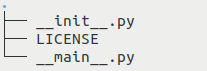
\includegraphics[width=4.5cm]{mon_package_poetry.png}

qui correspond en fait au dossier \textbf{mon\_package} dans l'arborescence du package.

\item Lorsque l'utilisateur télécharge l'archive du package à partir de PyPI, sa structure est la suivante 

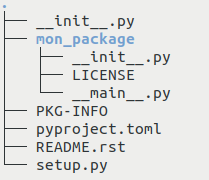
\includegraphics[width=4.5cm]{mon_package_poetry_archive.png}

On remarque que le dossier \textbf{dist} relatif à la création de la distribution a bien évidemment disparu, ainsi que le dossier \textbf{tests} et le fichier \textbf{poetry.lock} qui a servi à fixer la version des dépendances. A partir du répertoire d'installation \textbf{mon\_package.egg-info}, seul le fichier \textbf{PKG-INFO} a été conservé.

L'archive du package ne sera, dans ce cas, pas installée. Elle sera, en revanche, présente par défaut dans le dossier \textbf{Téléchargements} de l'ordinateur. Cela signifie que l'exécution du package par l'instruction standard

\begin{verbatim}
  python -m  mon_package
\end{verbatim} 

ne fonctionne pas car le système n'est pas en mesure de trouver le package à l'emplacement prévu des packages.

A partir du dossier \textbf{Téléchargements}, l'utilisation de l'instruction 

\begin{verbatim}
  python mon_package
\end{verbatim}

sans le "-m" ne fonctionne pas non plus, car l'interpréteur qui ne considère pas \texttt{mon\_package} comme un package et ne cherche pas le fichier \textbf{\_\_main\_\_.py} pour l'exécuter.

En revanche, si on se place à l'intérieur de l'archive, l'utilisation de l'instruction

\begin{verbatim}
  python __main__.py
\end{verbatim}

exécute le package en tant que programme. Cela n'a que peu d'intérêt vu qu'on attend d'un package qu'il s'exécute simplement sans qu'on ait à chercher préalablement son emplacement.

\end{itemize}

En conséquence, il est nécessaire pour l'utilisateur d'installer le package sur son ordinateur à l'emplacement réservé pour les packages afin de pouvoir l'exécuter. C'est le rôle de la distribution compilée \textbf{mon\_package-0.1.0-py3-none-any.whl} qui va s'exécuter avec l'instruction

\begin{verbatim}
  pip install mon_package
\end{verbatim}  

On peut dès lors entrevoir une confusion possible pour définir la racine du package. Pour l'utilisateur, la racine pourrait se trouver au niveau du module \textbf{\_\_main\_\_.py} si il installe le package, ou au niveau du fichier \textbf{pyproject.toml} si il télécharge le package. Dans le reste de ce document, nous considérons que la racine du package se trouve au niveau du fichier \textbf{pyproject.toml}, et que tous les chemins d'accès ont pour référence le module d'exécution primaire \textbf{\_\_main\_\_.py}.

Au moment de la construction du package
\begin{itemize}
\item le fichier \textbf{pyproject.toml} doit obligatoirement se trouver à la racine du package pour que les métadonnées du package puissent être interprétées.
\item le module \textbf{\_\_main\_\_.py} doit obligatoirement se trouver à l'intérieur du répertoire \\\textbf{mon\_package} pour qu'il soit effectivement installé et puisse être exécuté prioritairement.
\end{itemize}






% FONCTIONNEMENT D'UN PACKAGE -----------------
\section{Fonctionnement d'un package}

Il est possible d'utiliser les packages de différentes manières. 
\begin{itemize}
\item certains packages peuvent \textit{s'importer} (partiellement ou en totalité) en début de code afin d'en appeler les méthodes dans un module. On parle de \textit{import packages}.
\item d'autres packages sont \textit{exécutables} suivant une interface graphique ou suivant une interface en lignes de commandes. On parle de \textit{distribution packages}. C'est le cas de CRISPRbuilder\_TB qui s'installe et s'exécute en lignes de commandes à partir du répertoire courant. Ainsi, c'est à partir du répertoire courant qu'on appelle les modules et fichiers se trouvant à l'intérieur du package, lui-même installé à l'emplacement prévu pour les packages. Ce processus est transparent pour l'utilisateur qui n'a nul besoin de connaître l'emplacement de téléchargement de ses packages. Il est toutefois essentiel pour le développeur de connaître les chemins d'accès vers les modules d'un package, qui sont différentes des chemins d'accès vers les modules d'un programme local. On peut commencer par développer et tester le package en utilisant des chemins locaux, mais dès que celui-ci est prêt à être installé, il faut modifier ces chemins pour que n'importe quel ordinateur puisse exécuter le package convenablement.
\end{itemize}

Dans un programme local, le code s'exécute dans un répertoire courant et accède aux différents modules et fichiers support en utilisant un chemin relatif à ce répertoire courant ou encore en utilisant un chemin absolu. Les différentes dépendances sont importées en début de code, sans référence à un chemin d'accès car elles ont préalablement été installées dans l'environnement de développement de l'interpréteur Python. Dans le cas où on utilise un environnement de développement intégré tel que PyCharm, Spyder, Pydev, Wing, ..., il faut en plus les installer dans cet environnement.

Dans un package en revanche, c'est le module \textbf{\_\_main\_\_.py} qui est cherché par l'interpréteur et exécuté prioritairement. Prenons l'exemple concret du package CRISPRbuilder\_TB. Le module \textbf{\_\_main\_\_.py} se trouve dans le dossier \textbf{crisprbuilder\_tb} à l'emplacement prévu pour les pakages, indépendamment du répertoire courant. Il s'agit la plupart du temps de \\\textbf{$\sim$/.local/lib/python3.8/site-packages} ou encore \textbf{$\sim$/.local/lib/python3.8/dist-packages}. \\Lorsque \textit{Anaconda} est installé et que son environnement est activé par défaut au démarrage de la machine, cet emplacement devient \textbf{$\sim$/anaconda3/bin}. L'utilisateur ne trouvera aucun dossier du nom de \textbf{crisprbuilder\_tb} dans le répertoire courant après installation du package, bien qu'il l'ait installé à partir du répertoire courant. On peut chercher l'emplacement exact du package et le déplacer ensuite, mais ceci n'a aucun intérêt vu que le système mémorise l'emplacement de ses packages.

Afin d'expliquer le fonctionnement interne d'un package, nous conservons l'exemple de CRISPRbuilder\_TB. L'utilisateur se place dans son répertoire courant, exécute 

\begin{verbatim}
  python -m crisprbuilder_tb --collect ERR2704808
\end{verbatim}

qui va chercher le package CRISPRbuilder\_TB à son emplacement de stockage \textbf{$\sim$/anaconda3/bin} et l'exécute comme si celui-ci se trouvait dans le répertoire courant. Ainsi le module \textbf{\_\_main\_\_.py} s'exécute et appelle les modules \textbf{fonctions.py}, \textbf{bdd.py} et les fichiers du répertoire \textbf{data}. On pourrait définir des chemins d'accès absolus vers ces modules et fichiers, mais ces chemins seraient différents pour chaque système d'exploitation. On définit plutôt des chemins relatifs au module \textbf{\_\_main\_\_.py}, qui sert de référence pour les chemins d'accès. Ainsi, tous les fichiers et modules sont atteignables grâce à une adresse relative commençant par une variable d'environnement qui ne contient pas le nom du package \texttt{crisprbuilder\_tb}, car l'exécution du code se trouve déjà dans le package lors de la lecture du fichier \textbf{\_\_main\_\_.py}. Par exemple le chemin

\begin{verbatim}
  P_REP = path.join(path.dirname(__file__), 'REP')
\end{verbatim}

utilise la variable d'environnement \_\_file\_\_ qui définit un chemin relatif au fichier courant (le fichier \textbf{\_\_main\_\_.py}) suivi du dossier \textbf{REP}.

En revanche, l'importation des modules et fichiers du package en début de code doit tenir compte du nom du package. On trouve ainsi dans les premières lignes du module \textbf{\_\_main\_\_.py}

\begin{verbatim}
  import crisprbuilder_tb
  import crisprbuilder_tb.fonctions as fonctions
  import crisprbuilder_tb.bdd as bdd
\end{verbatim}

Bien évidemment, l'importation des dépendances en début de code reste indépendante du package CRISPRbuilder\_TB qui ne sera donc pas cité :

\begin{verbatim}
  import subprocess 
  from argparse import ArgumentParser
  from csv import reader, writer, QUOTE_MINIMAL
  from os import remove, listdir, rename, system, name, path
  from pathlib import Path 
  from pathlib import PurePath
  from shutil import rmtree, move
\end{verbatim}

Em conclusion, il est important de comprendre que l'exécution du package :
\begin{itemize}
\item \textbf{ne se fait pas} depuis l'intérieur du package avec l'instruction \texttt{python \_\_main\_\_.py}, qui ne permet pas d'utiliser les options du package.
\item \textbf{ne se fait pas} depuis le répertoire parent du package avec l'instruction \\\texttt{python crisprbuilder\_tb \textemdash \textemdash collect ERR2704808} sans le "-m". Dans ce cas, l'interpréteur ne va pas considérer \texttt{crisprbuilder\_tb} comme un package et ne va pas chercher le fichier \textbf{\_\_main\_\_.py} pour l'exécuter.
\item \textbf{se fait} à partir du répertoire courant, en utilisant l'instruction \texttt{python -m crisprbuilder\_tb \textemdash \textemdash collect ERR2704808}. C'est à l'ordinateur d'aller chercher le package à son emplacement de stockage. Tous les chemins décrits dans le code sont des chemins relatifs au module \\\textbf{\_\_main\_\_.py}.
\end{itemize}





% QUELLE LICENCE CHOISIR ------------------
\section{Quelle licence choisir ?}
	
Trois \index{licence}licences retiennent notre attention. En voici les principales caractéristiques :
\begin{itemize}
\item	la licence MIT, courte et permissive, préserve exclusivement le copyright et les avis de licence. Toute modification ultérieure peut être distribuée suivant une licence différente et notamment utilisée à des fins personnelles ou commerciales, sans obligation de publication des codes source,
\item	la licence Apache (2.0) est également permissive et sensiblement similaire dans ses conditions à la licence MIT. Toutefois, elle requiert de préciser les modifications effectuées lors de nouvelles distributions,
\item	la licence GNU (GPL v3.0) préserve également le copyright et les avis de licence. Elle peut être utilisée à des fins personnelles et commerciales. Elle impose en outre, en cas de modification, la publication complète des codes et l'utilisation de la licence GNU pour les nouvelles distributions.
\end{itemize}

Dans le cadre de ce projet, aucune spécification restrictive n'étant requise, nous avons choisi la licence MIT qui est simple et peu contraignante. Nous l'incorporons dans le fichier \textbf{LICENSE}.




% CHOIX DES OUTILS -----------------------------
\chapter{Le choix des outils}





% L'OUTIL D'EMPAQUETAGE --------------------
\section{L'outil d'empaquetage}
	
	Le PyPA recommande l'utilisation de :
\begin{itemize}
\item \textit{setuptools} pour définir des projets et créer des sources de distribution. Il gère les formats \textit{.egg} et les dépendances.
\item \textit{pip} pour l'installation de distributions à partir de PyPI, en tenant compte des dépendances. Certains packages sont référencés sur l'index sans que les distributions ne soient disponibles sur PyPI, et il est également possible de télécharger les distributions à partir d'URL définies dans un fichier \textbf{setup.py}.
\item \textit{pipenv} pour la gestion des dépendances de packages lors du développement d'applications,
\item \textit{venv} pour isoler les dépendances particulières d'une application et créer un environnement de développement.
\item \textit{pyenv} pour la gestion des versions de Python.
\item \textit{conda} permettant de fournir un environnement de développement favorable aux projets scientifiques, avec notamment tous les modules essentiels pré-installés.
\item \textit{buildout} pour les projets de développement Web.
\item \textit{poetry} pour un besoin particulier non couvert par \textit{pipenv}. \textit{Poetry} constitue en fait le nouveau standard de création de packages.
\end{itemize}

Au regard de ces recommandations, nous avons testé les outils préceédents dans le but de définir un environnement de développement et de construire un package incorporant les dépendances requises.

\textit{pipenv} est un gestionnaire de haut niveau pour les environnements, les dépendances et les packages Python. Contrairement à \textit{virtualenv}, \textit{pipenv} distingue les dépendances du projet et les dépendances des dépendances du projet. Par ailleurs, \textit{pipenv} différencie le mode développement du mode production. Il offre l'avantage de bien fonctionner sur Windows. Toutefois, la communauté Python l'a peu mis à jour depuis 2018.

\textit{Anaconda} est une distribution de logiciels multiplateformes (Windows, Linux, macOS) qui comprend une version de Python et facilite l'installation des librairies scientifiques \textit{Numpy, Pandas, Matplotlib} et \textit{Scipy}, ce qui est particulièrement intéressant dans le cas des plateformes Windows où ce processus est plus complexe. \textit{Anaconda} incorpore une librairie open-source appelée \textit{conda} permettant la gestion des dépendances, de l'environnement de travail ainsi que la création de packages. \textit{Anaconda} évite les problèmes d'installation de packages et de dépendances qui sont gérées de façon plus individualisée avec \textit{pip}. \textit{Anaconda} semble donc être appropriée au projet, mais c'est une distribution trop lourde pour être intégrée à notre package. \textit{Miniconda} est une distribution plus légère, qui comporte essentiellement Python et \textit{conda}, mais ne permet pas toujours d'installer toutes les dépendances d'un package comme nous le verrons ultérieurement. L'utilité d\textit{Anaconda} est avérée dans le cadre de la création de l'environnement de développement et durant les tests d'installation, comme nous le verrons ultérieurement. Toutefois, en raison de son poids important, nous ne pouvons pas l'intégrer au package.

Nous avons tout d'abord cherché à construire le package manuellement, à partir de \textit{pipenv} associé à \textit{pip}, puis de \textit{conda} qui dispose d'une riche bibliothèque. Cet effort s'est avéré laborieux et a révélé des incompatibilités lors du \textit{build} qui n'ont pas permis de valider les exigences de la plateforme \textit{testPyPI}.

Nous avons donc décidé de construire notre package en utilisant \textit{Poetry}, comme cela est maintenant recommandé sur Internet. \textit{Poetry} est un outil complet multiplateformes autour duquel la communauté Python reste très active. Il propose à la fois la gestion des dépendances, le \index{packaging}packaging\footnote{\textbf{packaging:} il s'agit de la création d'une structure pour un projet, de la génération de fichiers de configuration et de manifestes} et la publication. \textit{Poetry} automatise ces différents processus et facilite grandement le travail. Nous étudions en détail l'utilisation de cet outil dans le chapitre suivant.





% L'ENVIRONNEMENT DE DEVELOPPEMENT -----------------------------
\section{L'environnement de développement}

Les packages s'installent par défaut à l'adresse \textbf{$\sim$/.local/lib/python3.8/site-packages}, et différentes versions d'un même package peuvent donc se retrouver dans le même dossier. Ce qui peut conduire à utiliser la mauvaise version d'une dépendance et entraîner le dysfonctionnement d'un projet. Pour résoudre ce problème, les environnements de développement permettent d'installer les dépendances de projets différents à des adresses différentes tenant compte de chaque environnement. Ainsi plus aucune confusion n'est possible concernant la version d'une dépendance.

Avant de créer le package CRISPSbuilder\_TB, il faut commencer par construire un programme qui fonctionne localement sur une machine correctement paramétrée. Pour cela, nous définissons un \index{environnement de développement}environnement de développement, qui nous sert à exécuter le code et à le tester au fur et à mesure de son élaboration. Cet environnement contient tous les modules et packages nécessaires à son bon fonctionnement, c'est à dire les dépendances du projet.
 
L'outil de création d'environnement virtuel \index{venv}\textit{venv} nous permet de créer cet environnement de développement afin de tester les codes du projet. \textit{venv} commence par constituer un dossier contenant tous les exécutables nécessaires à l'utilisation des modules d'un projet Python. 

Dans le cadre de notre étude, nous créons un répertoire \textbf{biologie}, nous nous plaçons à l'intérieur puis nous créons, à l'aide de \textit{venv}, un environnement de développement \textbf{env\_bio} avec l'instruction suivante
\begin{verbatim}  cd biologie
  python -m venv env_bio\end{verbatim}

Dans cet environnement vient d'être créé le répertoire \textbf{bin} comprenant notamment le fichier\textbf{ activate}, qui permet d'activer les fonctionnalités de notre environnement.
Cette activation ne peut se faire qu'à partir du répertoire parent \textbf{biologie}. Il faut ensuite se placer à l'intérieur de \textbf{env\_bio} pour définir les modules utiles à l'environnement. Ceci se traduit par l'instruction
 \begin{verbatim}  source env_bio/bin/activate
  (env_bio)  cd env_bio\end{verbatim}

De nombreux systèmes d'exploitation incorporent Python 2.7 par défaut. Il convient donc de définir une version 3 de Python dans cet environnement de développement, et dans le cadre de notre projet une version 3.7 ou supérieure. Pour cela, le module \textit{pyenv} \index{pyenv} nous permet de définir une version de Python comme version locale de travail dans l'environnement. 

On peut choisir parmi les versions disponibles, grâce à l'instruction
\begin{verbatim}  pyenv install --list\end{verbatim}
La liste étant particulièrement longue, on peut éventuellement être plus spécifique en demandant les versions allant de 3.6 à 3.8 avec l'instruction
\begin{verbatim}  pyenv install --list | grep " 3\.[678]"\end{verbatim}

L'installation de la version 3.8.0 par exemple se fait grâce à l'instruction
\begin{verbatim}  pyenv install -v 3.8.0\end{verbatim}

La version 3.8.0 de Python se trouve maintenant installée dans \textbf{$\sim$/.pyenv/versions/}

Pour connaître toutes les versions de Python installées par pyenv, il suffit d'exécuter l'instruction suivante qui fournit une liste de résultats
\begin{verbatim}    pyenv versions
  * system
    2.7.10
    3.6.2
    3.8.0\end{verbatim}
où le caractère "*" indique la version active dans le répertoire courant.

On peut alors choisir la version 3.8.0 pour notre environnement de travail. Il suffit de se placer dans cet environnement et d'exécuter l'instruction
\begin{verbatim}  cd env_bio
  pyenv local 3.8.0\end{verbatim}

On peut vérifier que l'environnement a bien configuré la version 3.8.0 en exécutant de nouveau

\begin{verbatim}    pyenv versions
    system
    2.7.10
    3.6.2
  * 3.8.0\end{verbatim}

ou encore avec l'instruction
\texttt{python \textemdash-version} qui
permet de connaître quelle version de Python est utilisée dans le répertoire courant, qu'on se trouve dans un environnement de développement ou non.

En fait, \textit{pyenv} s'insère dans la variable d'environnement \$PATH et devient l'exécutable appelé par le système d'exploitation. On peut voir que l'interpréteur Python utilise bien cet environnement \textit{pyenv} pour appeler Python si on utilise l'instruction

\begin{verbatim}
  which python
\end{verbatim}

qui renvoie \textbf{$\sim$/.pyenv/shims/python} au lieu de \textbf{/usr/bin/python}.

On peut également choisir de mettre à jour la version de Python pour toute la machine, et de définir Python 3 comme étant la version par défaut. On utilise dans ce cas les instructions

\begin{verbatim}
  sudo apt-get install python 3.8.0
  alternatives --list | grep -i python
  alternatives --install /usr/bin/python python /usr/bin/python3.8 1
  alternatives --install /usr/bin/python python /usr/bin/python2.7 2
  python --version
  python 3.8.0
\end{verbatim}

Cette méthode est certes plus facile, mais peut engendrer des problèmes de fonctionnement du système pour certaines applications qui utilisent la version 2 de Python ou encore une version 3 spécifique.

Finalement, nous installons dans notre environnement de développement les dépendances nécessaires grâce à l'outil \textit{pip}\index{pip} qui les recherche directement dans PyPI :
\begin{itemize}
\item \begin{verbatim}  pip install xmltodict\end{verbatim}
le module \textit{xmltodict} permet de lire du code XML comme si il s'agissait de code JSON. Il permet donc une lecture plus rapide des fichiers.
\item  \begin{verbatim}  pip install openpyxl\end{verbatim}
le package \textit{openpyxl} permet de lire et d'écrire dans des fichiers Excel au format \textit{xlsx, xlsm, xltx} ou \textit{xltm}. Il comprend les modules \textit{et-xmlfile} et \textit{jdcal}. Il sera utile pour lire et transformer des fichier Excel mais ne sera pas nécessaire pour le fonctionnement du package.
\item  \begin{verbatim}  pip install xlrd\end{verbatim}
le module \textit{xlrd} extrait des données d'un tableur Excel à partir de la version 2.0 et avant de les formatter.
\item  \begin{verbatim}  pip install biopython\end{verbatim}
le package \textit{biopython} regroupe un ensemble d'outils Python pour le traitement informatique de la biologie moléculaire et comprend le module numpy.
\item \begin{verbatim}  pip install parallel-fastq-dump\end{verbatim}
le package \textit{parallel-fastq-dump} permet de téléchargement de fichiers fasta en utilisant plusieurs threads simultanément. Il procure donc un gain de temps à l'application. Le dépôt \url{https://github.com/rvalieris/parallel-fastq-dump} préconise l'installation de \textit{parallel-fastq-dump} via l'outil \textit{conda}.
\item \begin{verbatim}  pip install blastn+\end{verbatim}
le package \textit{blast} permet de trouver des régions similaires entre plusieurs séquences biologiques. Le programme compare en fait des séquences de protéines ou de nucléotides à une base de données du NCBI afin d'en calculer la signification statistique.
\end{itemize}

Pour connaître l'emplacement où ces packages se sont installés, il est possible d'utiliser le script Python en lignes de commande

\begin{verbatim}
  python
  import site
  site.getsitepackages()
\end{verbatim}

qui peut par exemple renvoyer comme réponse

\begin{itemize}
\item \textbf{$\sim$/.local/lib/python3.8/site-packages} 
\item \textbf{$\sim$/.local/lib/python3.8/dist-packages}
\item \textbf{$\sim$/.pyenv/versions/3.8.0/lib/python3.8/site-packages}
\item \textbf{$\sim$/venv/lib/python3.8/site-packages} 
\item \textbf{$\sim$/anaconda3/bin}
\end{itemize}

On remarque ainsi qu'en fonction du type d'environnement de développement utilisé, les packages ne s'installent plus à l'adresse par défaut \textbf{$\sim$/.local/lib/python3.8/site-packages}.

On peut obtenir une information plus détaillée au sujet d'un package (par exemple \textit{biopython}) à l'aide de l'instruction

\begin{verbatim}
  pip show biopython
\end{verbatim}

qui renvoie comme réponse 

\begin{verbatim}
  Name: biopython
  Version: 1.77
  Summary: Freely available tools for computational molecular biology.
  Home-page: https://biopython.org/
  Author: The Biopython Contributors
  Author-email: biopython@biopython.org
  License: UNKNOWN
  Location: /home/stephane/.pyenv/versions/3.8.0/lib/python3.8/site-packages
  Requires: numpy
  Required-by: crisprbuilder-tb
\end{verbatim}

On remarque, en plus de l'emplacement, la dépendance \textit{numpy} ainsi que le package \textit{crisprbuilder\_tb} dont \textit{biopython} constitue une dépendance.

Notons que certains modules utilisés dans CRISPRbuilder\_TB sont nativement présents dans la librairie standard Python 3, et il n'est donc pas nécessaire de les installer séparément. Ils sont installés en tant que \textit{system packages} et non pas \textit{site packages}. C'est le cas par exemple de
\begin{itemize}
\item du module \textit{os} qui fournit une manière portable d'utiliser les fonctionnalités dépendantes du système d'exploitation,
\item du module \textit{pickle} qui permet de sérialiser et désérialiser une structure d'objet Python. Il remplace le module primitif \textit{marshal},
\item du module \textit{csv} qui implémente des classes pour lire et écrire des données liées à des feuilles de calcul ou des bases de données au format \textit{.csv},
\item du module \textit{shutil} qui propose des opérations sur les fichiers et collections de fichiers, notamment la copie et suppression de fichiers,
\item du module \textit{subprocess.run} qui permet de gérer de nouveaux processus, de se connecter à leurs flux d'input/output/erreurs. Il remplace plusieurs modules dépréciés : \textit{os.system, os.spawn*, os.popen*, popen2.*, commands.* },
\item du module \textit{pathlib} qui fournit des classes de chemins purs indépendants du système d'exploitation, ce qui permet au code de manipuler des chemins sans accéder au système d'exploitation,
\item du module \textit{argparse} qui gère la création et l'utilisation d'interfaces en ligne de commande.
\end{itemize}

Le package CRISPRbuilder\_TB, une fois installé par l'utilisateur, devra fournir un environnement de travail similaire à celui que nous venons de construire, c'est à dire que les dépendances nécessaires à son bon fonctionnement devront également être installées. 

On pourrait par exemple retrouver les modules installés via \textit{pip} dans un fichier \textbf{requirements.txt} construit en gelant l'état de l'environnement à un moment précis grâce à une instruction du type 
\begin{verbatim}  pip freeze > requirements.txt\end{verbatim}

L'utilisateur pourrait alors installer ces modules à l'identique en utilisant l'instruction
\begin{verbatim}  pip install -r requirements.txt\end{verbatim}

Cette méthode fonctionne bien pour construire un environnement de développement à partir d'un répertoire courant où se trouve le fichier \textbf{requirements.txt}. C'est d'ailleurs la technique que nous avons utilisée pour construire notre environnement. Toutefois, elle n'est pas adaptée à l'installation des dépendances de CRISPRbuilder\_TB par un utilisateur,  car celui-ci devrait trouver l'emplacement du package, s'y rendre pour ensuite exécuter \texttt{pip install -r requirements.txt}.

Ce processus d'installation devrait rester transparent pour l'utilisateur. C'est pourquoi, il devrait être pris en charge par un gestionnaire de package tel que \textit{Poetry} regroupant les versions des dépendances dans un fichier \textbf{pyproject.toml} qui remplace \textbf{requirements.txt}. Nous verrons au cours des tests d'installation que les dépendances ne sont pas toujours reconnues à partir de \textit{Poetry} et qu'il est quand même nécessaire pour l'utilisateur d'avoir préalablement installé et paramétré sur sa machine les outils du SRA Toolkit \textit{parallel-fastq-dump}, \textit{blast} et \textit{blastn}. CRISPRbuilder\_TB étant destiné à un public de bio-informaticiens, ce prérequis devrait déjà être installé sur l'ordinateur des utilisateurs du package. Il convient toutefois de le préciser dans la documentation d'installation \textbf{crisprbuilder\_tb.ipynb}.





% PARAMETRAGE DE L'ENVIRONNEMENT ------------------
\section{L'environnement de développement avec Anaconda}

Nous venons de voir qu'il est possible de créer un environnement de développement adapté à notre projet, sans modifier le reste de la structure de notre machine. C'est d'ailleurs cette méthode que nous avons initialement utilisée. Toutefois, cet environnement nécessite un paramétrage de la variable d'environnement \$PATH afin que les modules recherchés puissent être trouvés par le système au moment de l'exécution du package. Afin que ce paramétrage reste permanent, il faut modifier cette variable d'environnement à l'intérieur même du \textbf{$\sim$/.bashrc} en utilisant l'instruction

\begin{verbatim}
  echo $PATH
  export PATH=$PATH:~/.local/bin/python3.8/site-packages
\end{verbatim}

ou selon le chemin d'accès choisi

\begin{verbatim}
  echo $PATH
  export PATH=$PATH:~/venv/lib/python3.8/site-packages
\end{verbatim}

Il existe une alternative plus simple qui a retenu notre attention seulement à la fin du projet. Cela consiste à installer le package \textit{Anaconda}, qui comprend notamment l'outil \texttt{conda} et le module \textit{bioconda} dont nous aurons besoin. Il faut ensuite installer toutes les dépendances du projet à l'aide de \texttt{conda}. Ces dépendances s'installent systématiquement dans \textbf{$\sim$/anaconda3/bin} et la variable d'environnement \$PATH se met automatiquement à jour. Le package CRISPRbuilder\_TB étant destiné à un public de bio-informaticiens, il est fort probable que ces derniers aient déjà installé \textit{Anaconda} sur leur machine, car il s'agit d'un outil classique de travail dans un environnement scientifique.  

Attention toutefois de ne pas installer conjointement \textit{Anaconda} avec \textit{Miniconda}. En effet, dans ce cas certaines dépendances s'installent dans \textbf{$\sim$/anaconda3/bin} et d'autres dans \textbf{$\sim$/miniconda/bin}. C'est tentant au début, car \textit{Miniconda} est une distribution légère qui donne accès à l'outil \texttt{conda} et au module \textit{bioconda}. Toutefois, ce dernier utilise le Cloud d'\textit{Anaconda} pour installer certaines dépendances de notre projet, ce qui rend l'installation d'\textit{Anaconda} nécessaire. Pour éviter tout problème de chemin d'accès, il faut alors désinstaller \textit{Miniconda} avant d'installer \textit{Anaconda}. 

L'installation de \textit{Anaconda} est décrite sur le site \url{https://docs.anaconda.com/anaconda/install/linux/}. Il faut penser à ordonner les priorités des différents \textit{channels}, dont notamment \textit{bioconda} en ajoutant dans l'ordre

\begin{verbatim}
  conda config --add channels defaults
  conda config --add channels bioconda
  conda config --add channels conda-forge
\end{verbatim}

 Il convient ensuite d'installer toutes les dépendances du projet
\begin{verbatim}  conda install -c conda-forge xmltodict
  conda install -c anaconda openpyxl
  conda install -c anaconda xlrd
  conda install -c anaconda biopython
  conda install -c bioconda parallel-fastq-dump
  conda install -c bioconda blast
  conda install -c kantorlab blastn\end{verbatim}

Notons que, contrairement au choix de créer un environnement local de développement, \textit{Anaconda} propose un environnement de travail scientifique pour l'ensemble de la machine. Par ailleurs, il s'installe avec sa propre version de Python, qui est nécessairement récente. Lorsqu'il est paramétré pour être exécuté par défaut, les packages se placent dans son environnement à l'adresse \textbf{$\sim$/anaconda3/bin}.


	


% POETRY ---------------
\chapter{Construction du package avec Poetry}


Pour construire notre package, nous avons suivi les explications fournies par le site \url{https://python-poetry.org/} qui fait référence. Nous nous sommes également inspiré du dépôt \url{https://github.com/python-poetry/poetry}.


% CREATION DU PACKAGE --------
\section{Création du package}

Pour créer notre projet, il ne faut pas commencer par définir un dossier du nom du package, car cela sera automatiquement fait par \index{Poetry}\textit{Poetry}. Il suffit d'exécuter l'instruction

\begin{verbatim}
  poetry new crisprbuilder_tb
\end{verbatim}

qui permet de générer le squelette de l'application contenant les éléments suivants.

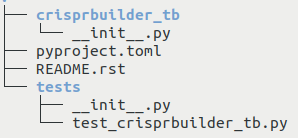
\includegraphics[width=6cm]{nom_package_tree.png}

\begin{itemize}
\item le répertoire \textbf{crisprbuilder\_tb} contient initialement le fichier \textbf{\_\_init\_\_.py} et c'est dans ce répertoire que nous allons rajouter tous les composants principaux du code, à savoir \\\textbf{\_\_main\_\_.py}, \textbf{fonctions.py}, \textbf{bdd.py} et les répertoires \textbf{data}, \textbf{doc}, \textbf{REP}, \textbf{sequences} et \textbf{tmp} avec leurs contenus. En effet, la création de l'archive va compresser ce répertoire \textbf{crisprbuilder\_tb} afin de le publier. Nous rajoutons également dans le répertoire \textbf{doc} une \textbf{LICENSE} qui pourra être consultée par l'utilisateur. Par ailleurs, la version 3.3 de Python a introduit la notion de \textit{Implicit Namespace Packages}, qui permet la création de packages sans la présence de fichiers \textbf{\_\_init\_\_.py}. Nous supprimons donc le fichier \textbf{\_\_init\_\_.py} du répertoire \textbf{crisprbuilder\_tb}.  %Nous choisissons d'insérer des fichiers \textbf{\_\_init\_\_.py} vides dans CRISPRbuilder\_TB, car nous verrons qu'ils sont créés automatiquement lors de la construction du package. Pour éviter tout conflit de version avec le fichier \textbf{pyproject.toml}, nous vidons le fichier \textbf{\_\_init\_\_.py} du répertoire \textbf{crisprbuilder\_tb}. Lors de sa création, le fichier\textbf{\_\_init\_\_.py} contenait uniquement la version du package.
\item le fichier \textbf{pyproject.toml} se trouve à la racine du package. 
\item le fichier \textbf{README.rst} fournit une brève description du package, et nous le modifions au format markdown \textbf{README.md} pour des raisons pratiques.  
\item nous rajoutons à la racine du package un fichier \textbf{.gitignore} pour la gestion des versions avec l'outil \textit{Git}.
\item nous supprimons le fichier \textbf{\_\_init\_\_.py} du répertoire \textbf{tests}. %Nous précisons dans le fichier \textbf{\_\_init\_\_.py} le bon numéro de version
\end{itemize}

Notons qu'il est préférable de choisir un nom de package en minuscules pour éviter toute confusion car, bien que les majuscules soient conservées sur PyPI, l'appel du package en ligne de commande devra s'effectuer en minuscules. En outre, par convention il faut éviter le symbole '-' qui est automatiquement remplacé par '\_' lors de la création du package.

Notre projet ressemble maintenant à ceci

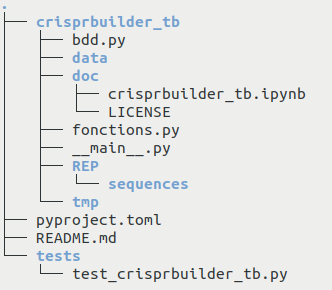
\includegraphics[width=7cm]{crispr_etape2.png}









% GESTION DES DEPENDANCES ----
\section{Gestion des dépendances}

Pour chaque dépendance, \textit{Poetry} va choisir la version la plus récente compatible avec les autres dépendances du package. Ce processus est automatisé en utilisant l'instruction 

\begin{verbatim}
  poetry add nom_dependance
\end{verbatim}

après s'être placé dans le répertoire \textbf{crisprbuilder\_tb}. La dépendance \texttt{nom\_dependance} avec sa version est alors incorporée dans le fichier \textbf{pyproject.toml}, le fichier \textbf{poetry.lock} est créé, afin de fixer la version de cette dépendance. Il est également possible d’imposer certaines contraintes sur les versions des dépendances en les incorporant manuellement dans le fichier \textbf{pyproject.toml}.

%\begin{tcolorbox} \end{tcolorbox}
Il faut maintenant ajouter les dépendances suivantes au projet :
\begin{verbatim}  cd crisprbuilder_tb 
  poetry add xlrd 
  poetry add xmltodict 
  poetry add biopython
  poetry add parallel-fastq-dump \end{verbatim}

Le fichier \textbf{pyproject.toml} comporte donc les versions suivantes

\begin{verbatim}  [tool.poetry.dependencies]
  python = "^3.6"
  xlrd = "^1.2.0"
  xmltodict = "^0.12.0"
  biopython = "^1.77"
  parallel-fastq-dump = "^0.6.5"
  blast = "^2.10.1"
  blastn = "^2.7.1"
\end{verbatim}

Notons que la version de Python se complète automatiquement d'après celle utilisée par défaut lors de l'appel au module \textit{Poetry}. On peut toutefois la changer manuellement dans le fichier \textbf{pyproject.toml}, ce que nous faisons en imposant a minima la version 3.6, récente mais encore assez répandue. On peut également compléter manuellement ce fichier pour fournir des informations d'ordre général du type

\begin{verbatim}  [tool.poetry]
  name = "crisprbuilder_tb"
  version = "0.1.2"
  description = "Collect and annotate Mycobacterium tuberculosis WGS data for CRISPR 
  investigations."
  authors = ["stephane-robin <robin.stephane@outlook.com>"]
  license = "MIT"
  readme = "README.md"
  homepage = "https://github.com/stephane-robin/crisprbuilder_tb.git"
  repository = "https://github.com/stephane-robin/crisprbuilder_tb.git"
  keywords = ["tuberculosis", "CRISPR"]\end{verbatim}

La rubrique [tool.poetry.dev-dependencies] définit le module qui procèdera aux tests concernant le fonctionnement du package.

La rubrique [build-system] définit les versions de \textit{Poetry} et \textit{poetry.masonry.api} nécessaires à la construction du package.

Notre projet dispose maintenant de la structure suivante

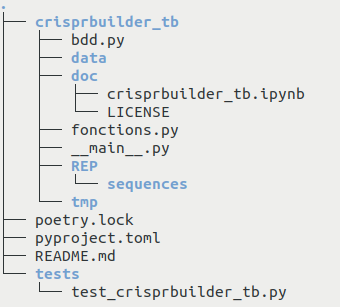
\includegraphics[width=7cm]{crispr_etape2-1.png}

Pour installer ensuite les dépendances du projet au sein du package, il est nécessaire d’utiliser l’instruction

\begin{verbatim}
  poetry install
\end{verbatim}

qui crée le fichier \textbf{setup.py} à partir de \textbf{pyproject.toml}. Ce fichier \textbf{setup.py} va servir à créer automatiquement le répertoire \textbf{crisprbuilder\_tb.egg-info}, comprenant le code, les ressources et les métadonnées du projet.

Lors de l'exécution du code \texttt{poetry install}, on constate également que \textit{Poetry} crée en fait un environnement virtuel dans lequel il va installer les dépendances et le package

\begin{verbatim}  poetry install
  Creating virtualenv crisprbuilder-tb-oJzk4q3N-py3.8 in ~/.cache/pypoetry/virtualenvs
  Installing dependencies from lock file

  Package operations: 14 installs, 0 updates, 0 removals

  - Installing pyparsing (2.4.7)
  - Installing six (1.14.0)
  - Installing atomicwrites (1.4.0)
  - Installing attrs (19.3.0)
  - Installing more-itertools (5.0.0)
  - Installing numpy (1.18.4)
  - Installing packaging (20.3)
  - Installing pluggy (0.13.1)
  - Installing py (1.8.1)
  - Installing wcwidth (0.1.9)
  - Installing biopython (1.76)
  - Installing pytest (4.6.9)
  - Installing xlrd (1.2.0)
  - Installing xmltodict (0.12.0)
  - Installing parallel-fastq-dump (0.6.5)
  - Installing crisprbuilder_tb (0.1.26)
  - Installing blast (2.10.1)
  - Installing blastn (2.7.1)
\end{verbatim}

Notons qu'on peut s'assurer à ce moment-là de la version de Python utilisée pour tout le travail de construction, à savoir dans cet exemple Python 3.8 qui apparaît à la fin de \\\texttt{crisprbuilder-tb-oJzk4q3N-py3.8}.

Notre projet dispose maintenant de la structure suivante

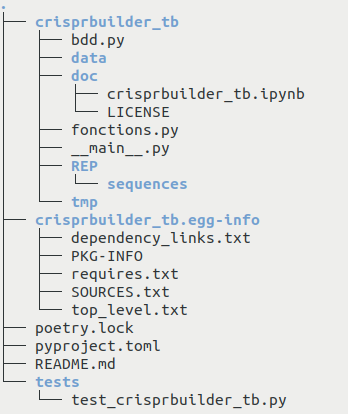
\includegraphics[width=7.5cm]{crispr_etape3.png}





% CONSTRUCTION DU PACKAGE -----
\section{Construction du package}

Pour empaqueter le projet, il faut utiliser l’instruction

\begin{verbatim}
  poetry build
\end{verbatim}

qui va permettre de créer un répertoire source \textbf{dist} contenant une archive \textbf{crisprbuilder\_tb-0.1.2.tar.gz} et une distribution compilée \textbf{crisprbuilder\_tb-0.1.2-py3-none-any.whl}, à partir du répertoire \textbf{crisprbuilder\_tb} et du fichier d'installation \textbf{crisprbuilder\_tb.egg-info}. Lors de l'exécution du code \texttt{poetry build}, on constate bien la constitution des fichiers mentionnés

\begin{verbatim}  poetry build
  Building crisprbuilder_tb (0.1.2)
    - Building sdist
    - Built crisprbuilder_tb-0.1.2.tar.gz

    - Building wheel
    - Built crisprbuilder_tb-0.1.2-py3-any.whl\end{verbatim}

Attention, si la distribution comporte la mention "py2" au lieu de "py3", cela signifie que la construction sous \textit{Poetry} a été réalisée à partir de Python 2. Il faut donc bien s'assurer, avant la création du package, de choisir une version de Python 3 dans le fichier \textbf{pyproject.toml}.

On peut vérifier la conformité du package avec l’instruction
\texttt{poetry check}
qui renvoie
\texttt{All set !}
si le package ne comporte aucune discordance et peut être publié.

Notre package présente maintenant la structure suivante avant d'être publié

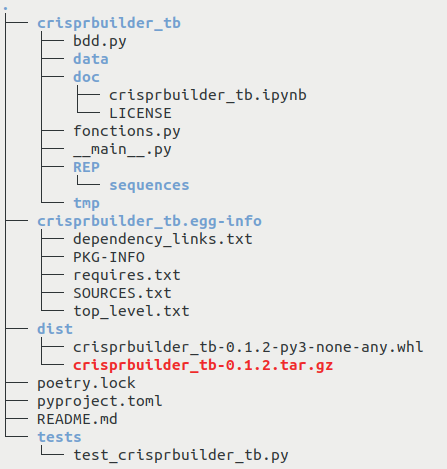
\includegraphics[width=9cm]{crispr_etape4.png}






% PUBLICATION -----
\section{Publication du package}

Lorsque le package est finalement prêt pour être publié sur PyPI, on utilise l’instruction

\begin{verbatim}  poetry publish\end{verbatim}

Pour cela, l'auteur du package doit être enregistré sur PyPI avec un identifiant et un mot de passe. A partir de ce moment-là, le package est rendu disponible publiquement. On peut l'installer avec l'outil \textit{pip} ou en télécharger l'archive. Le répertoire \textbf{dist} est enregistré sur PyPI à la rubrique "Download files" qui contient les fichiers \textbf{crisprbuilder\_tb-0.1.2.tar.gz} et \textbf{crisprbuilder\_tb-0.1.2-py3-none-any.whl}.

On peut bien évidemment publier une nouvelle version du package sur PyPI ou encore le supprimer. En revanche, par mesure de sécurité, il n'est pas possible de modifier une version du package ou de re-créer un package du même nom que celui déjà supprimé. 

On pourra retrouver un cas concret simple de publication de package avec \textit{Poetry} dans le tutoriel que nous avons publié à l'adresse suivante : \href{http://www.youtube.com}{http://www.youtube.com}





% LA STRUCTURE DE L'ARCHIVE DU PACKAGE -------------------------
\section{La structure de l'archive du package}

Le fichier \textbf{crisprbuilder\_tb-0.1.2.tar.gz} est une archive qui, une fois décompressée contient les éléments suivants :

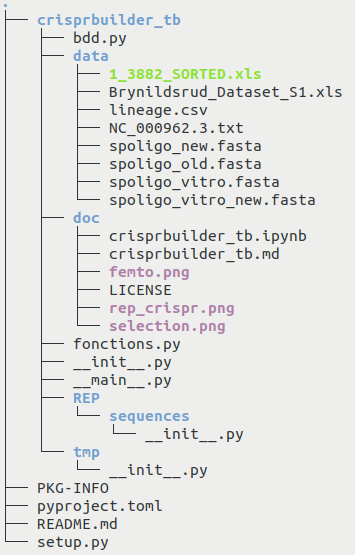
\includegraphics[width=7cm]{tar.png}

On constate une arborescence assez semblable à celle obtenue lors de la création du package. Toutefois, les dossiers \textbf{crisprbuilder\_tb.egg-info}, \textbf{dist}, \textbf{tests} et le fichier \textbf{poetry.lock}, nécessaires à la construction et l'installation du package, ont bien évidemment disparu. Du répertoire \textbf{crisprbuilder\_tb.egg-info} a été uniquement conservé le fichier \textbf{PKG.INFO}. Le fichier \textbf{setup.py} est également archivé.

\begin{itemize}
\item un répertoire \textbf{doc} comprenant la documentation nécessaire pour comprendre et utiliser convenablement le package,
\item un répertoire \textbf{\_\_pycache\_\_} comprenant les fichiers compilés correspondant aux fichiers \textbf{\_\_main\_\_.py}, \textbf{fonctions.py} et \textbf{bdd.py},
\item un répertoire \textbf{data} comprenant les bases de données utiles au programme,
\item un répertoire \textbf{REP} comprenant un répertoire \textbf{sequences} qui contiendra les résultats de recherche concernant les différents SRA,
\item un répertoire \textbf{tmp} qui contiendra, entre autres, un fichier \textbf{nb.txt}, différent pour chaque SRA
\item les fichiers \textbf{\_\_main\_\_.py}, \textbf{fonctions.py} et \textbf{bdd.py}, immédiatement accessibles.
\end{itemize}





%  LA STRUCTURE DU PACKAGE INSTALLE ----
\section{La structure du package installé}

Une \textit{built distribution} est une distribution pré-construite contenant des fichiers et méta-données qui ne nécessite pas d'étape supplémentaire pour s'installer dès lors qu'on l'enregistre au bon emplacement. Il ne s'agit pourtant pas d'une distribution pré-compilée. Les formats \textit{egg} et \textit{wheel} sont des \textit{built distributions}.

Une \textit{source distribution} est une distribution au format \textit{sdist} contenant des fichiers et méta-données qui génère une \textit{built distribution} au moment de l'installer avec \textit{pip}.

Ainsi, \textit{pip} va installer CRISPRbuilder\_TB en cherchant préférentiellement un fichier au format \textit{wheel}, c'est à dire dans le cas présent \textbf{crisprbuilder\_tb-0.1.2-py3-none-any.whl}. Si un tel fichier n'existait pas, \textit{pip} en construirait un à partir d'une \textit{source distribution} puis le conserverait en mémoire en vue d'une prochaine installation, pour éviter d'avoir à le reconstruire. Les fichiers au format \textit{wheel} permettent donc une installation plus rapide du package.

Afin de connaître la structure de CRISPRbuilder\_TB une fois installé, et bien qu'il ne soit pas nécessaire pour l'utilisateur de se rendre à l'emplacement prévu pour les packages, nous nous rendons à l'adresse \textbf{$\sim$/anaconda3/bin/cripsrbuilder\_tb} où la structure suivante apparaît

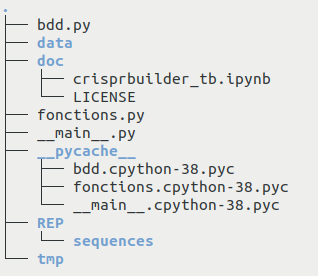
\includegraphics[width=7cm]{crispr_installe.png}

Nous remarquons, par rapport à l'archive \textbf{crisprbuilder\_tb-0.1.2.tar.gz}, que seul le contenu du répertoire \textbf{crisprbuilder\_tb} a été conservé. Ainsi, les fichiers de construction \textbf{PKG-INFO}, \textbf{pyproject.toml} et \textbf{setup.py} ont naturellement disparu. Le fichier \textbf{README.md} a également disparu. Il a servi uniquement à compléter la section \textit{Project description} sur PyPI. On pourrait l'inclure dans le répertoire \textbf{crisprbuilder\_tb} afin que l'utilisateur puisse le consulter. Toutefois, cela ne semble pas utile, vu qu'il est déjà présent en ligne sur PyPI et qu'une documentation plus exhaustive existe déjà dans l'archive du package, à savoir \textbf{crisprbuilder\_tb.ipynb}.




% RESUME ----------------
\section{Résumé des instructions Poetry}

\begin{tabular}{|l|l|}
\hline
\textbf{Instructions en lignes} & \textbf{Effet obtenu}\\
\textbf{de commandes} & \\
\hline
\texttt{poetry new crisprbuilder\_tb} & création du package, des dossiers \textbf{crisprbuilder\_tb} et \textbf{tests}, \\
& des fichiers \textbf{pyproject.toml} et \textbf{README.rst}\\
\hline
\texttt{poetry add xlrd} & rajout de la dépendance \textit{xlrd} dans \textbf{pyproject.toml} et \\
& création du fichier \textbf{poetry.lock}\\
\hline
\texttt{poetry install} & création du fichier \textbf{setup.py} à partir de \textbf{pyproject.toml} et\\
& création du répertoire \textbf{crisprbuilder\_tb.egg-info}  et de \\
& ses méta-données à partir du fichier \textbf{setup.py}\\
\hline
\texttt{poetry build} & création du répertoire \textbf{dist}, des fichiers \\
& \textbf{crisprbuilder\_tb-0.1.2.tar.gz} et \\
& \textbf{crisprbuilder\_tb-0.1.2-py3-none-any.whl} à partir des\\
& méta-données du répertoire  \textbf{crisprbuilder\_tb.egg-info}\\
\hline
\texttt{poetry publish} & enregistrement en ligne des fichiers\\
& \textbf{crisprbuilder\_tb-0.1.2.tar.gz} et \\
&  \textbf{crisprbuilder\_tb-0.1.2-py3-none-any.whl}\\
\hline
\texttt{pip install crisprbuilder\_tb} & installation du package à partir du \\
& fichier \textbf{crisprbuilder\_tb-0.1.2-py3-none-any.whl}\\
\hline
\end{tabular}



% LE PACKAGE CRISPRBUILDER --------------------------------
\chapter{La documentation du package \\(version originale)}


La création d'un package nécessite l'élaboration d'une documentation détaillée en anglais permettant de bien comprendre son fonctionnement. Une documentation trop succincte ou peu détaillée aurait pour conséquence le manque d'intérêt pour le package ou une incompréhension légitime qui démotiverait ses utilisateurs.

Cette documentation doit comporter trois volets :
\begin{itemize}
\item une \textit{docstring} inclue dans le code au début de chaque fonction et de chaque module,
\item un fichier \textbf{README.md} servant de description succincte du package pour le site de PyPI,
\item une documentation détaillée \textbf{crisprbuilder\_tb.ipynb} qu'on peut retrouver sur le dépôt \url{https://github.com/stephane-robin/crisprbuilder_tb/blob/master/crisprbuilder_tb/doc/crisprbuilder_tb.ipynb}, et qui est également inclue dans le package sous le répertoire \textbf{doc}.
\end{itemize}   

Nous présentons ci-dessous cette documentation détaillée dans sa version originale en anglais.


\includegraphics[width=5cm]{femto.png}

The CRISPRbuilder\_TB package is an open source software made available
under generous terms. Please see the LICENSE file for further details.

If you use CRISPRbuilder\_TB in a study contributing to a scientific
publication, we ask that you cite the following application note:
Femto-ST Institute, UMR 6174 CNRS, University of Bourgogne
Franche-Comté, France.

This package originated in the work of Section \cite{guyeux1} and
Section \cite{guyeux2}.



% PURPOSE OF THIS PACKAGE ----------------
    \section{Purpose of this package}\label{purpose-of-this-package}

    CRISPRbuilder\_TB will help you collect and annotate Mycobacterium
tuberculosis whole genome sequencing data for CRISPR investigations.
Given a Sequence Read Archive reference, the package will provide the
genome information dictionary comprised of the following elements:

\begin{itemize}
\item
  the reads - number of reads for the study, length of those reads,
  coverage of the study,
\item
  the study - source of publication for the SRA reference, authors who
  discovered it, location of discovery, date of discovery, center that
  discovered the SRA, reference of the study, study accession number,
\item
  identity - name of the SRA reference, strain for the SRA, taxid,
  bioproject number,
\item
  spoligotypes - description, numbers, new version numbers, vitro
  description, vitro numbers, vitro new version description, vitro new
  version numbers, Spoligotype International Type, Spoligotype
  International Type silico,
\item
  lineages - Coll et al. 2014 (for all lineages) Section \cite{coll-preston},
  Stucki et al. 2016 (for Lineage 4) Section \cite{stucki-brites},
  Palittapongarnpim et al. 2018 (for Lineage 1) Section \cite{pali-ajaw},
  Shitikov et al. 2017 (for Lineage 2) Section \cite{shiti-kolchenko}.
\end{itemize}


% HOW TO INSTALL THE PACKAGE ------------------------
    \section{How to install the package
?}\label{how-to-install-the-package}

Make sure your system is set to Python 3 in your current directory and \textit{pip} is set to work with Python 3, before using the \texttt{pip} instruction and executing the package. The default version of Python on your computer might be different. You can also check that \textit{pip} is linked to Python3 by writing \texttt{pip \textemdash \textemdash version}, which will display a line similar to

\begin{verbatim}
pip 20.1.1 from ~/pyenv/versions/3.8.0/lib/python3.8/site-packages/pip (python 3.8)
\end{verbatim}

When installing CRISPRbuilder\_TB, the following dependencies will be automatically installed, and there will be no further action to take:
\begin{itemize}
\item xmltodict
\item xlrd
\item biopython
\item numpy
\end{itemize}

Please note that CRISPRbuilder\_TB requires a recent version of Python 3 (3.6 or higher), and the installation process will seek such a version.

Prior to the installation, it is important that your system is correctly set to use NCBI tools \textit{parallel-fastq-dump} and \textit{blast}. The installation process will require these dependencies, but will not set the environment variable \$PATH to find them on your system. You will need to do it manually by updating the \textit{$\sim$/.bashrc} like it is explained in \url{https://opensource.com/article/17/6/set-path-linux}. We recommand that you use \textit{Anaconda}, which provides a simple way to update the \$PATH and download these packages using the command lines

\begin{verbatim}
  conda install -c bioconda parallel-fastq-dump
  conda install -c bioconda blast
  conda install -c kantorlab blastn
\end{verbatim}

    This package comes with a Command Line Interface, so it should be
installed and executed using your command prompt. For Linux, macOS or
Windows platforms, the installation requires the same instructions. From your current directory, execute the following line

    \begin{verbatim}
  pip install crisprbuilder_tb
\end{verbatim}

    Please note that \texttt{cripsrbuilder\_tb} is written without capital
letters in the command prompt.

First the program will download the last version of CRISPRbuilder\_TB, and the dependencies \textit{xmltodict, parallel-fastq-dump, xlrd, biopython, numpy}. Then it will install the dependencies and the package.

\begin{verbatim}  Collecting crisprbuilder_tb
  Collecting xmltodict<0.13.0,>=0.12.0 (from crisprbuilder_tb)
  Collecting xlrd<2.0.0,>=1.2.0 (from crisprbuilder_tb)
  Collecting parallel-fastq-dump<0.7.0,>=0.6.5 (from crisprbuilder_tb)
  Collecting biopython <2.0,>=1.77 (from crisprbuilder_tb)
  Collecting numpy (from biopython<2.0,>=1.77->crisprbuilder_tb)
  Installing collected packages: xmltodict, xlrd, parallel-fastq-dump, numpy, 
  biopython, crisprbuilder_tb
  Successfully installed biopython-1.77 crisprbuilder_tb-1.2.0 numpy-1.19.0 
  parallel-fastq-dump-0.6.5 xlrd-1.2.0 xmltodict-0.12.0
\end{verbatim}

 It is not necessary to first install the dependencies, since CRISPRbuilder\_TB will deal with them on its own.

If a previous version of CRISPRbuilder\_TB already exists on your computer, you can upgrade it using 

\begin{verbatim}
  pip install --upgrade crisprbuilder_tb
\end{verbatim}

If this instruction doesn't work, you can force the upgrade by first removing the package before installing it again

\begin{verbatim}
  pip uninstall crisprbuilder_tb
  pip install crisprbuilder_tb
\end{verbatim}

You can also choose a specific version of the package on PyPI, like for example

\begin{verbatim}
  pip install crisprbuilder_tb==1.2.0
\end{verbatim}

CRISPRbuilder\_TB is not referrenced in the Anaconda Cloud. So it is not possible to install the package with the instruction

\begin{verbatim}
  conda install crisprbuilder_tb
\end{verbatim}


% HOW TO USE THE COMMAND LINE INTERFACE --------------------
    \section{How to use the Command Line Interface
?}\label{how-to-use-the-command-line-interface}

    After installing the package, you can find help by using the command prompt,
listing the different available options, such as \texttt{-\/-collect},
\texttt{-\/-list}, \texttt{-\/-add}, \texttt{-\/-print},
\texttt{-\/-remove}, \texttt{-\/-change}, and their expected syntax.
Stay in the current directory and write in the
command prompt

    \begin{verbatim}
  python -m crisprbuilder_tb --help
\end{verbatim}

    The help menu will display the following information:

    \begin{verbatim}
  usage: crisprbuilder_tb [-h] [--collect] [--list] [--add] [--remove] [--change]
  [--print] sra

  Collects and annotates Mycobacterium tuberculosis whole genome sequencing data
  for CRISPR investigation.

  positional arguments:
    sra         requires the reference of a SRA, the path to a file of SRA 
                references or 0. See doc.

  optional arguments:
    -h, --help  show this help message and exit
    --collect   collects the reference of a SRA to get information about this SRA. 
                See doc.
    --list      collects the path to a file of SRA references to get information 
                about. See doc.
    --add       collects data to add to the file data/lineage.csv. Requires 0 as 
                argument. See doc.
    --remove    removes data from the file data/lineage.csv. Requires 0 as 
                argument. See doc.
    --change    collects data to update the file data/lineage.csv. Requires 0 as
                argument. See doc.
    --print     prints the file data/lineage.csv. Requires 0 as argument. See doc.
\end{verbatim}



% EXECUTING CRISPRBUILDER_TB WITH A SRA REFERENCE ------------
    \subsection{Executing CRISPRbuilder\_TB with a SRA
reference}\label{executing-crisprbuilder_tb-with-a-sra-reference}

    You can run the package if you wish to find information regarding a
specific SRA. From your current directory, write in the command prompt:

    \begin{verbatim}
  python -m crisprbuilder_tb --collect {SRA_reference}
\end{verbatim}

    Please note the importance of "-m" to run \texttt{crisprbuilder\_tb} as a
package, otherwise the interpreter will look at \texttt{crisprbuilder\_tb} as a folder inside the current folder and not as a package. CRISPRbuilder\_TB uses version 3 of Python, so make sure your system is set to Python 3 in your current directory before using the
\texttt{python} instruction. The default version on your computer might
be different.

\textbf{Caution:} it is not recommanded to find the location of the
package and go to the directory containing \textbf{crisprbuilder\_tb} in order to
execute it. If you do so, the above instructions won't work.

    \textbf{Exemple:} to find information about SRR8368696, write:

    \begin{verbatim}
  python -m crisprbuilder_tb --collect SRR8368696
\end{verbatim}


% EXECUTING CRISPRBUILDER_TB WITH A LIST OF SRA REFERENCES -----
    \subsection{Executing CRISPRbuilder\_TB with a list of SRA
references}\label{executing-crisprbuilder_tb-with-a-list-of-sra-references}

    To run the package with a list of SRA references, this list must be
composed of one SRA reference per line in a \textit{.txt} format file. Then, if
you wish to find information regarding a list of specific SRAs, stay in
the directory containing the package and write in the command prompt:

    \begin{verbatim}
  python -m crisprbuilder_tb --list {path_to_the_file}
\end{verbatim}

    \textbf{Exemple:} to find information about the different SRAs included
in the file \textbf{my\_file.txt} from the \textbf{Documents} directory,
write:

    \begin{verbatim}
  python -m crisprbuilder_tb --list /Documents/my_file.txt
\end{verbatim}



% PRINTING THE DATABASE LINEAGE.CSV --------------------------
    \subsection{Printing the database
lineage.csv}\label{printing-the-database-lineage.csv}

    If you want to consult the \textbf{lineage.csv} database, stay in the
directory containing the package and write in the command prompt:

    \begin{verbatim}
  python -m crisprbuilder_tb --print 0
\end{verbatim}

    \textbf{Caution:} it is necessary to add the 0 after \texttt{-\/-print}.

The program will then display the content of the database
\textbf{lineage.csv} whose extract can be found below:

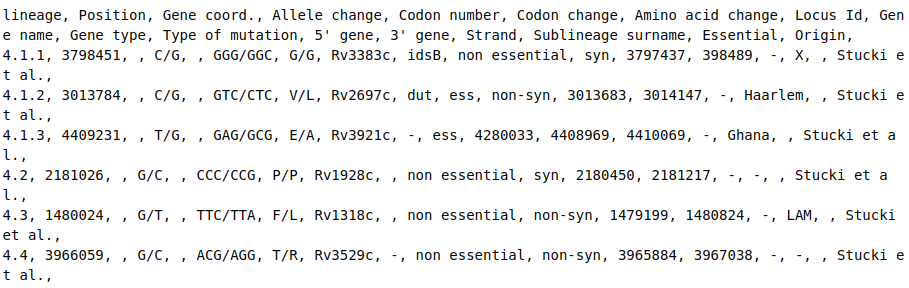
\includegraphics[width=16cm]{img_01.png}



% ADDING A RECORD TO LINEAGE.CSV ------------------------
    \subsection{Adding a record to
lineage.csv}\label{adding-a-record-to-lineage.csv}

    If you want to add a record to the \textbf{lineage.csv} database, stay
in the current directory and write in the command prompt:

    \begin{verbatim}
  python -m crisprbuilder_tb --add 0
\end{verbatim}

    \textbf{Caution:} it is necessary to add the 0 after \texttt{-\/-add}.

You will then be asked the values of the different fields (lineage,
position, gene coordinates, allele change, codon number, codon change,
amino acide change, locus ID, gene name, gene type, type of mutation, 5'
gene, 3' gene, strand, sublineage surname, essential, origin of the
study). If you don't know the value of a particular field, just
press enter.



% REMOVING A RECORD FROM LINEAGE.CSV -------------------------------
    \subsection{Removing a record from
lineage.csv}\label{removing-a-record-from-lineage.csv}

    If you want to remove a record from the \textbf{lineage.csv} database,
stay in the current directory and write in the command
prompt:

    \begin{verbatim}
  python -m crisprbuilder_tb --remove 0
\end{verbatim}

    \textbf{Caution:} it is necessary to add the 0 after
\texttt{-\/-remove}.

After confirming the removal, you will be asked for the reference
of the line you wish to delete, which consists of the lineage and the
position (see below). If you don't know this reference, you can always
print the \textbf{lineage.csv} database beforehand to find it.

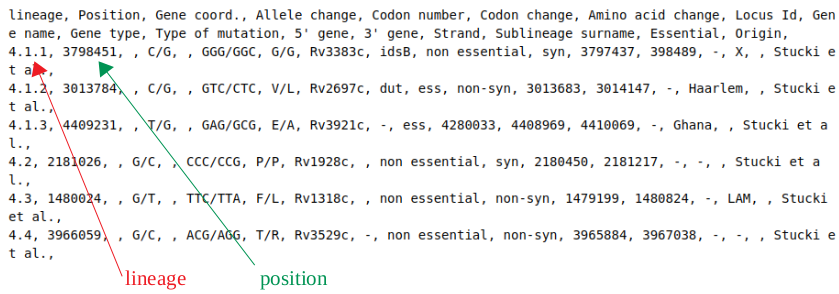
\includegraphics[width=16cm]{selection.png}

    The execution of the code will end with:

    \begin{verbatim}
  The line has been removed.
\end{verbatim}

    or

    \begin{verbatim}
  Your request was cancelled.
\end{verbatim}

    in case the SRA reference is not correct.


% CHANGING A RECORD ------------------------
    \subsection{Changing a record from
lineage.csv}\label{changing-a-record-from-lineage.csv}

    If you want to change a record from the \textbf{lineage.csv} database,
stay in the current directory and write in the command
prompt:

    \begin{verbatim}
  python -m crisprbuilder_tb --change 0
\end{verbatim}

    \textbf{Caution:} it is necessary to add the 0 after
\texttt{-\/-change}.

After confirming the change, you will be asked for the reference of
the line you wish to delete, which consists of the lineage and the
position (see below). If you don't know the reference, you can always
print the \textbf{lineage.csv} database beforehand to find it.

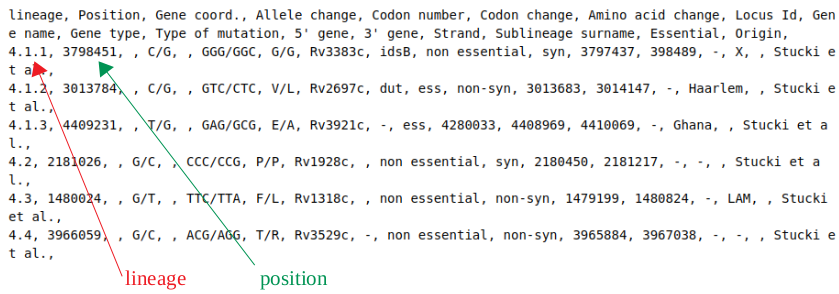
\includegraphics[width=16cm]{selection.png}

    You will then be asked the values of the different fields: lineage,
position, gene coordinates, allele change, codon number, codon change,
amino acide change, locus ID, gene name, gene type, type of mutation, 5'
gene, 3' gene, strand, sublineage surname, essential, origin of the
study. If you don't know the value of a particular field, just
press enter.

    The execution of the code will end with:

    \begin{verbatim}
  The line has been changed.
\end{verbatim}

    or

    \begin{verbatim}
  Your request was cancelled.
\end{verbatim}


% COMPOSITION OF THE PACKAGE AND DEPENDENCIES -------------
    \section{Composition of the package and
dependencies}\label{composition-of-the-package-and-dependencies}

    CRISPRbuilder\_TB needs the following dependencies to work:

\begin{itemize}
\item
  python = "\^{}3.6.4"
\item
  xlrd = "\^{}1.2.0"
\item
  openpyxl = "\^{}3.0.3"
\item
  xmltodict = "\^{}0.12.0"
\item
  biopython = "\^{}1.76"
\item
  datetime = "\^{}4.3"
\item
  parallel-fastq-dump
\item
  blast
\item
  blastn
\end{itemize}

These different versions are automatically downloaded when installing
CRISPRbuilder\_TB. Please note that this package doesn't support Python
2.

    The package structure is the following:

    \begin{itemize}
\item
  The \textbf{\_\_main\_\_.py} and \textbf{fonctions.py} files contain
  the actual code for the package,
\item
  the \textbf{bdd.py} file contains the Origines dictionary,
\item
  The \textbf{data} directory contains the necessary database to compare
  with the SRA reference when the code is executed,
\item
  The \textbf{REP/sequences} directory contains the different result
  database for each execution of the code. For example, you can find a
  directory \textbf{ERR2704808} containing the fasta files \textbf{ERR2704808\_1.fasta},
  \textbf{ERR2704808\_2.fasta} and \textbf{ERR2704808\_shuffled.fasta} along with the
  files \textbf{ERR2704808.00.nhr}, \textbf{ERR2704808.00.nin}, \textbf{ERR2704808.00.nsq},\\
  \textbf{ERR2704808.nal} and the directory \textbf{ERR2704808} containing the blast
  database. That's typically where you can find the files
  \textbf{ERR2704808\_old.blast} and \textbf{ERR2704808\_new.blast}.
\item
  The \textbf{doc} directory contains the necessary documentation to
  explain how this package works. It includes the copyright conditions for this package with the
  \textbf{LICENSE} file and the present documentation.
\end{itemize}

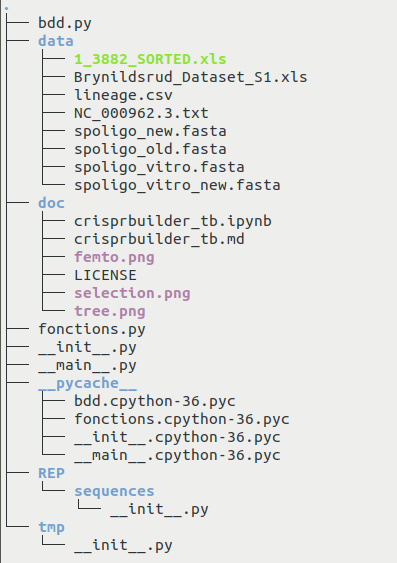
\includegraphics[width=8cm]{rep_crispr.png}



% RETRIEVING THE GENOME INFORMATION -------------------
    \section{Retrieving the genome information
dictionary}\label{retrieving-the-genome-information-dictionary}

    Let's assume you're looking for information regarding ERR2704808. After
writing \texttt{python\ -m\ \\crisprbuilder\_tb\ -\/-collect\ ERR2704808}
in the command prompt, a directory called\\ \textbf{ERR2704808} will be
created in \textbf{REP/sequences} and the item ERR2704808 will be added
to the database. The following message will be displayed:

    \begin{verbatim}
  We're creating a directory ERR2704808.
  We're adding ERR2704808 to the database.
\end{verbatim}

    Then the files in fasta format will be downloaded to
\textbf{REP/sequences/ERR2704808} as in the following code:

\begin{verbatim}
  if len([u for u in listdir(rep) if 'fasta' in u]) == 0:
      print("We're downloading the files in fasta format")

      try:
          completed = subprocess.run(['parallel-fastq-dump', '-t', '8',
                                      '--split-files', '--fasta', '-O', P_REP,
                                      '-s', item], check=True)
          completed.check_returncode()
          # if the download worked
          print("fasta files successfully downloaded.")
          for k in listdir(P_REP):
              if k.endswith('.fasta'):
                  p_item_k = str(PurePath(crisprbuilder_tb.__path__[0], 'REP',
                                          'sequences', item, k))
                  p_k = str(PurePath(crisprbuilder_tb.__path__[0], 'REP', k))
                  try:
                      move(p_k, p_item_k)
                  except FileNotFoundError:
                      print("We can't transfer the fasta files in the proper "
                            "repository.")
      except subprocess.CalledProcessError:
          # if the download didn't work, we delete the SRA from dico_afr
          del dico_afr[item]
          print("Failed to download fasta files.")
\end{verbatim}

    If \textbf{ERR2704808\_shuffled.fasta} is not in the \textbf{ERR2704808}
directory, then the\\ \textbf{ERR2704808\_1.fasta} and \textbf{ERR2704808\_2.fasta} files
will be mixed in a new\\ \textbf{ERR2704808\_shuffled.fasta} file in the
\textbf{ERR2704808} directory, as in the following code:

\begin{verbatim}
  p_shuffled = str(PurePath(crisprbuilder_tb.__path__[0], 'REP', 'sequences',
                            item, item + '_shuffled.fasta'))
      if item + '_shuffled.fasta' not in listdir(rep):

          print("We're mixing both fasta files, which correspond to the two "
                "splits ends.")

          p_fasta_1 = str(PurePath(crisprbuilder_tb.__path__[0], 'REP',
                                   'sequences', item, item + '_1.fasta'))
          p_fasta_2 = str(PurePath(crisprbuilder_tb.__path__[0], 'REP',
                                   'sequences', item, item + '_2.fasta'))

          if name == 'posix':
              system("sed -i 's/" + item + './' + item + "_1./g' " + p_fasta_1)
              system("sed -i 's/" + item + './' + item + "_2./g' " + p_fasta_2)
              system("cat " + p_fasta_1 + " " + p_fasta_2 + " > " + p_shuffled)
          else:
              fonctions.change_elt_file(p_fasta_1, '_1', item)
              fonctions.change_elt_file(p_fasta_2, '_2', item)
              fonctions.concat(p_fasta_1, p_fasta_2, p_shuffled)
\end{verbatim}

    The number of reads represented by '\textgreater{}' in
\textbf{ERR2704808\_shuffled.fasta} will be counted and assigned to \texttt{nb\_reads}, as
in the following code:

\begin{verbatim}
  if 'nb_reads' not in dico_afr[item] or dico_afr[item]['nb_reads'] == '':
      if name == 'posix':
          system("cat " + p_shuffled + " | grep '>' | wc -l > " + P_TXT_POSIX)
          nb_reads = eval(open(P_TXT_POSIX).read().split('\n')[0])
      else:
          with open(p_shuffled, 'r') as f_in, open(P_TXT_WIN, 'w') as f_out:
              lignes = f_in.readlines()
              cpt = 0
              for elt in lignes:
                  cpt += elt.count('>')
                  f_out.write(str(cpt))
          nb_reads = eval(open(P_TXT_WIN).read().split('\n')[0])

      dico_afr[item]['nb_reads'] = nb_reads
\end{verbatim}

    The length of the reads will be evaluated from
\textbf{ERR2704808\_shuffled.fasta} as in the following code:

\begin{verbatim}
  if 'len_reads' not in dico_afr[item]:
      nb_len = len(''.join(open(p_shuffled).read(10000).split('>')[1].split(
                   '\n')[1:]))
      dico_afr[item]['len_reads'] = nb_len
\end{verbatim}

    which eventually will be displayed by:

    \begin{verbatim}
  nb_reads: 14304698
  len_reads: 108
\end{verbatim}

    When starting the download, the following information will be displayed:

    \begin{verbatim}
  SRR ids: ['ERR2704808']
  extra args: ['--split-files', '--fasta']
  tempdir: /tmp/pfd_1a9adanv
  ERR2704808 spots: 7152349
  blocks: [[1, 894043], [894044, 1788086], [1788087, 2682129], [2682130, 3576172], 
  [3576173, 4470215], [4470216, 5364258], [5364259, 6258301], [6258302, 7152349]]
\end{verbatim}

    If the NCBI server is busy or your connection unstable, the following
message could show up:

    \begin{verbatim}
  2020-05-09T09:25:58 fastq-dump.2.8.2 sys: libs/kns/unix/syssock.c:606:
  KSocketTimedRead: timeout exhausted while reading file within network system 
  module - mbedtls_ssl_read returned -76 ( NET - Reading information from the 
  socket failed )
\end{verbatim}

    Ignore the message and let the program run. It might take a while, but
you'll eventually find that the download is processing correctly with
the following message:

    \begin{verbatim}
  Read 894043 spots for ERR2704808
  Written 894043 spots for ERR2704808
  fasta files successfully downloaded.
  We're mixing both fasta files, which correspond to the two splits ends.
\end{verbatim}

    The coverage will be calculated and, if it is too, low the procedure
will be cancelled:

 \begin{verbatim}
  if 'couverture' not in dico_afr[item] or \
          dico_afr[item].get('couverture') == '':
      dico_afr[item]['couverture'] = round(dico_afr[item].get('nb_reads') *
                                           dico_afr[item].get('len_reads') /
                                           TAILLE_GEN, 2)
        
  if dico_afr[item].get('couverture') < 50:
      del dico_afr[item]
      print(f"The coverage is too low. {item} is being removed from the "
            "database")
\end{verbatim}

    which will be displayed by:

    \begin{verbatim}
  couverture: 350.2        
\end{verbatim}

    Then, a database for blast will be created in
\textbf{REP/sequences/ERR2704808/ERR2704808}, \\as in the code:

\begin{verbatim}
  if item+'.nal' not in listdir(rep) and item+'.nin' not in listdir(rep):
      print("We're creating a database for Blast")
      try:
          completed = subprocess.run(['makeblastdb', '-in', p_shuffled,
                                      '-dbtype', 'nucl', '-title', item,
                                      '-out', repitem], check=True)
          completed.check_returncode()
      except subprocess.CalledProcessError:
          print("We can't proceed blasting file.")
\end{verbatim}

    You will then read the following message:

    \begin{verbatim}
  We're creating a database for Blast
  Building a new DB, current time: 05/09/2020 12:18:30
  New DB name:   /home/stephane/Biologie/env_bio/CRISPRbuilder-TB/REP/sequences/
  ERR2704808/ERR2704808
  New DB title:  ERR2704808
  Sequence type: Nucleotide
  Keep MBits: T
  Maximum file size: 1000000000B
  Adding sequences from FASTA; added 14304698 sequences in 1213.96 seconds.
\end{verbatim}

    Some research will eventually be made in the dataset \texttt{Brynildsrud},
according to the code:

\begin{verbatim}
  brynildsrud = fonctions.to_brynildsrud()
  if item in brynildsrud:
      for elt in brynildsrud[item]:
          dico_afr[item][elt] = brynildsrud[item][elt]
          print(f"{item} is in the database Brynildsrud")
  else:
      print(f"{item} is not in the database Brynildsrud")
\end{verbatim}

    If ERR2704808 doesn't belong to the dataset Brynildsrud, the following
message will appear:

    \begin{verbatim}
  ERR2704808 is not in the database Brynildsrud
\end{verbatim}

    Sequences from the fasta files will be added and the spoligotypes will
be blasted, as in the code:

\begin{verbatim}
  if 'spoligo' not in dico_afr[item] or dico_afr[item]['spoligo'] == '':
      print("The spoligotypes are being blasted")
      dico_afr[item]['spoligo'] = ''
      dico_afr[item]['spoligo_new'] = ''

      p_spoligo_old = str(PurePath(crisprbuilder_tb.__path__[0], 'data',
                                   'spoligo_old.fasta'))
      p_spoligo_new = str(PurePath(crisprbuilder_tb.__path__[0], 'data',
                                   'spoligo_new.fasta'))
      p_old_blast = str(PurePath(crisprbuilder_tb.__path__[0], 'tmp', item
                                 + "_old.blast"))
      p_new_blast = str(PurePath(crisprbuilder_tb.__path__[0], 'tmp', item
                                 + "_new.blast"))

      try:
          completed = subprocess.run("blastn -num_threads 12 -query " +
                                     p_spoligo_old + " -evalue 1e-6 -task "
                                     "blastn -db " + repitem + " -outfmt "
                                     "'10 qseqid sseqid sstart send qlen "
                                     "length score evalue' -out " +
                                     p_old_blast, shell=True, check=True)
          completed.check_returncode()
      except subprocess.CalledProcessError:
          print("We can't proceed blasting file.")

      try:
          completed = subprocess.run("blastn -num_threads 12 -query " +
                                     p_spoligo_new + " -evalue 1e-6 -task "
                                     "blastn -db " + repitem + " -outfmt "
                                     "'10 qseqid sseqid sstart send qlen "
                                     "length score evalue' -out " +
                                     p_new_blast, shell=True, check=True)
          completed.check_returncode()
      except subprocess.CalledProcessError:
          print("We can't proceed blasting file.")

      for pos, spol in enumerate(['old', 'new']):
          p_blast = str(PurePath(crisprbuilder_tb.__path__[0], 'tmp', item
                                 + '_' + spol + '.blast'))
          p_fasta = str(PurePath(crisprbuilder_tb.__path__[0], 'data',
                                 'spoligo_' + spol + '.fasta'))

          with open(p_blast) as file:
              matches = file.read()
              nb_max = open(p_fasta).read().count('>')
              for k in range(1, nb_max + 1):
                  if matches.count('espaceur' + spol.capitalize() + str(k)
                                   + ',') >= 5:
                      dico_afr[item]['spoligo' + ['', '_new'][pos]] \
                                     += '\u25A0'
                  else:
                      dico_afr[item]['spoligo' + ['', '_new'][pos]] \
                                     += '\u25A1'

          dico_afr[item]['spoligo' + ['', '_new'][pos] + '_nb'] = [
              matches.count('espaceur' + spol.capitalize() + str(k) + ',')
              for k in range(1, nb_max + 1)]
          try:
              move(p_blast, rep)
          except FileNotFoundError:
              print(p_blast, " is already in the SRA directory.")
\end{verbatim}

    You will read the message:

    \begin{verbatim}
  The spoligotypes are being blasted
  The spoligo-vitro are being blasted
\end{verbatim}

    The different files \textbf{ERR2704808\_*.blast} will then be moved to
\textbf{REP/sequences/ERR2704808}

    As a result, the programm will display the following information:

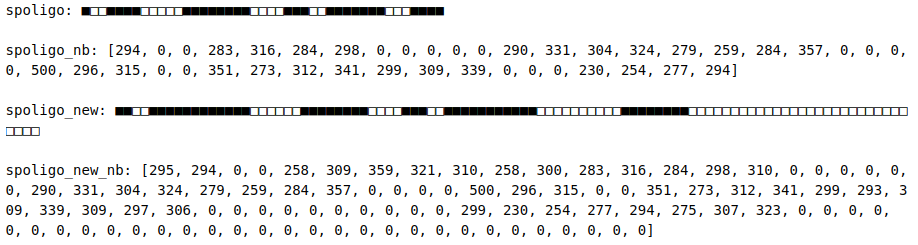
\includegraphics[width=16.5cm]{spoligo1.png}

    The same process is applied to the spoligotypes\_vitro.

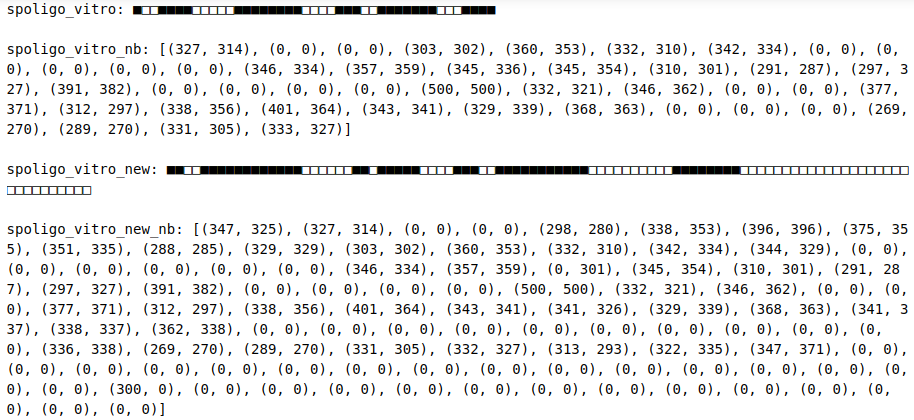
\includegraphics[width=16.5cm]{spoligo2.png}

    The Spoligotype International Type and Spoligotype International Type
silico will be retrieved using the following code:

\begin{verbatim}
  if 'SIT' not in dico_afr[item] or dico_afr[item]['SIT'] == '':
      fonctions.add_spoligo_dico('SIT', dico_afr, item, spol_sit)

  if 'SIT_silico' not in dico_afr[item]:
      fonctions.add_spoligo_dico('SIT_silico', dico_afr, item, spol_sit)
\end{verbatim}

    which will display the following message:

    \begin{verbatim}
  We're adding the SIT: X to the database
  We're adding the SIT_silico: X to the database
\end{verbatim}

    Finally, the lineage will be defined by comparing the blast files with
the different lineages L6+animal, Principal Genotyping Group, Principal
Genotyping Group-cp, Coll, Pali, Shitikov and Stucki, as for example in
the code:

\begin{verbatim}
  if 'lineage_Pali' not in dico_afr[item]:
      lignee = []
      lignee_snp = fonctions.to_reads('Pali')
      print("We're adding the lineage according to the SNPs Pali")

      for item2, pos0 in enumerate(lignee_snp):
          seq1, seq2 = lignee_snp[pos0][:2]
          p_blast = str(PurePath(crisprbuilder_tb.__path__[0], 'tmp',
                                 'snp_Pali.blast'))
          with open(fonctions.P_FASTA, 'w') as f_fasta:
              f_fasta.write('>\n' + seq2)
          cmd = "blastn -query " + fonctions.P_FASTA + " -num_threads 12" \
                " -evalue 1e-5 -task blastn -db " + repitem + \
                " -outfmt '10 sseq' -out " + p_blast
          system(cmd)
          with open(p_blast) as f_blast:
              formatted_results = f_blast.read().splitlines()

          nb_seq1 = fonctions.to_nb_seq(seq1, formatted_results, 16, 20,
                                        21, 25)
          nb_seq2 = fonctions.to_nb_seq(seq2, formatted_results, 16, 20,
                                        21, 25)

          if nb_seq2 > nb_seq1:
              lignee.append(lignee_snp[pos0][2])

      lignee = [u for u in sorted(set(lignee))]

      dico_afr[item]['lineage_Pali'] = lignee
\end{verbatim}

    During its work the program will display the following message:

    \begin{verbatim}
  We're adding the lineage according to the SNPs L6+animal
  We're adding the lineage according to the SNPs PGG
  The lineage is being updated.
  We're adding the lineage according to the SNPs Coll
  We have selected specific reads to compare with different lineages
  We're adding the lineage according to the SNPs Pali
  We have selected specific reads to compare with different lineages
  We're adding the lineage according to the SNPs Shitikov
  We have selected specific reads to compare with different lineages
  We're adding the lineage according to the SNPs Stucki
\end{verbatim}

    which will produce the following result:

    \begin{verbatim}
  lineage_L6+animal: 1
  lineage_PGG_cp: ['1', 'X']
  lineage_PGG: X
  lineage_Coll: ['4', '4.9', '5']
  lineage_Pali: ['1']
  lineage_Shitikov: []
  Lignee_Stucki: ['4.10']
\end{verbatim}

    Some general information will be retrieved from the dataset \texttt{Origines} or
directly from NCBI, using the code:

\begin{verbatim}
  if 'Source' not in dico_afr[item]:
      for ref in bdd.Origines:
          if item in ref['run accessions']:
              for elt in ['Source', 'Author', 'study accession number',
                          'location']:
                  dico_afr[item][elt] = ref.get(elt)

  if 'taxid' not in dico_afr[item]:
      dicobis = fonctions.get_info(item)
      for elt in dicobis:
          dico_afr[item][elt] = dicobis[elt]
\end{verbatim}

    If the SRA belongs to \texttt{Origines}, the following message will be displayed:

    \begin{verbatim}
  ERR2704808 is in the database Origines
\end{verbatim}

    which will produce the following result:

    \begin{verbatim}
  Source: Unexpected Genomic and Phenotypic Diversity of Mycobacterium africanum   
  Lineage 5 Affects Drug Resistance, Protein Secretion, and Immunogenicity
  Author: Ates et al. 2018
  study accession number: PRJEB25506
  location: France
  date: 2007
  SRA: ERS2280688
  center: DST/NRF Centre of Excellence for Biomedical TB research, SAMRC 
  Centre for TB Research
  strain: 
  taxid: 33894
  name: Mycobacterium tuberculosis variant africanum
  study: ena-STUDY-DST/NRF Centre of Excellence for Biomedical TB research, SAMRC 
  Centre for TB Research-10-03-2018-12:26:21:907-341
  bioproject: PRJEB25506
\end{verbatim}





% LES TESTS DU PACKAGE -----------------------
\chapter{Tester le package}

Les tests font partie du processus de développement et sont effectués dans chacune des phases de création du code afin de pouvoir continuer à l'étape suivante.

Plusieurs niveaux de tests doivent être effectués pour valider le package avant publication. Ils nécessitent un environnement de développement dont nous avons déjà parlé et un environnement de test. Celui-ci est re-créé pour chaque système d'exploitation faisant partie de la campagne de tests. Il ne doit pas contenir les dépendances de CRISPRbuilder\_TB, à l'exception de \textit{parallel-fastq-dump}, \textit{blast} et \textit{blastn} que nous installons à partir de \textit{Anaconda} par souci de simplicité. L'environnement de test intègre ainsi Python 3.7 qui est installé en même temps que \textit{Anaconda}.

Notre campagne de tests comporte les démarches suivantes :
\begin{itemize}
\item durant la création de chaque fonction, les \textbf{tests unitaires} sont effectués à l'aide de l'environnement de développement et du module \textit{Unittest},
\item au moment du regroupement du code et des différents modules, les \textbf{tests d'intégration} utilisent l'environnement de développement et la notation fournie par le module \textit{pylint},
\item lors d'une modification de code, les \textbf{tests de non-régression} utilisent l'environnement de développement, et notre travail est facilité par l'utilisation de l'outil de versioning \textit{Git},
\item lorsque le package est construit, les \textbf{tests de performance} et les \textbf{tests de validation} s'appuient également sur l'environnement de développement
\item les \textbf{tests d'installation} dépendent de chaque système d'exploitation et nécessitent autant d'environnements de tests que de systèmes. Nous simulerons les différents systèmes à l'aide de l'application \textit{VirtualBox}.
\item les \textbf{tests de configuration} pour déterminer les systèmes les mieux adaptés utilisent également un environnement de test.
\end{itemize}







% TESTS UNITAIRES ---------
\section{Les tests unitaires, le module unittest}

Les tests unitaires consistent à évaluer individuellement les composants de l'application (parties de code autonomes, fonctions, ...), en terme de qualité et validation des résultats attendus.

Il faut donc comprendre le fonctionnement, puis tester chaque portion de code et chaque fonction individuellement avec des paramètres choisis avant de l'incorporer dans le module \textbf{\_\_main\_\_.py}. 

Ce projet est également l'occasion de mieux comprendre la gestion des entrées/sorties en Python à partir de fichiers aux formats \textit{.fasta}, \textit{.xls}, \textit{.csv} et \textit{txt}. Avant de pouvoir traiter les données du répertoire \textbf{data}, il est nécessaire d'en changer le format de stockage, de les regrouper en un unique fichier, de les télécharger en vue d'écrire sur un fichier ou de lire ce fichier. Les tests unitaires se font souvent à partir de bases de données de tests temporaires pour éviter d'endommager les bases de données du package. 

Pour effectuer ces tests, nous utilisons le module \index{unittest}\textit{unittest} intégré dans la distribution standard de Python 3 qui fournit des outils pour construire et lancer les tests.





% UNITTEST ------
\section{unittest}

Le module \textit{unittest} utilise une approche orientée objet et propose les caractéristiques suivantes :

\begin{itemize}
\item gère l'automatisation et l'aménagement des tests, c'est à dire la création de bases de données temporaires, de répertoires, le démarrage de serveurs, le nettoyage des processus.
\item crée des scenari de tests, qui attendent des réponses spécifiques pour certaines entrées. La classe \textit{TestCase} permet de créer ces scenari.
\item organise les tests en collections de scenari de tests, et gère le partage de code pour la finalisation des tests.
\item utilise des lanceurs de tests sous forme d'interface graphique ou d'interface en lignes de commandes. Ces lanceurs de tests dirigent l'exécution des tests et fournissent les résultats.
\end{itemize}

Le module \textit{unittest} fonctionne essentiellement avec des méthodes d'assertion du type :

\begin{itemize}
\item \texttt{assertEqual(x, y)} qui vérifie que \texttt{x} est bien égal à \texttt{y}. 
\item \texttt{assertNotEqual(x, y)} qui vérifie que \texttt{x} est bien différent de \texttt{y}.
\item \texttt{assertTrue(x)} qui vérifie que \texttt{x} est le booleen True.
\item \texttt{assertFalse(x)} qui vérifie que \texttt{x} est le booleen False.
\item \texttt{assertIn(x, y)} qui vérifie que \texttt{x} appartient à \texttt{y}.
\item \texttt{assertNotIn(x, y)} qui vérifie que \texttt{x} n'appartient pas à \texttt{y}.
\item \texttt{assertRaises(excp, fonct, arg)} qui vérifie que \texttt{fonct(arg)} lève bien l'exception \texttt{excp}.
\end{itemize}

Un scénario de tests est une classe fille de \texttt{unittest.TestCase}. On définit pour cela une classe \texttt{CrisprMethods(unittest.TestCase)} contenant des méthodes dont le nom commence par \texttt{test}, qui permettent de valider le comportement de chacune des fonctions utilisées dans le package CRISPRbuilder\_TB. Pour cela, on peut recopier les différentes fonctions de CRISPRbuilder\_TB dans un module \textbf{main.py} à l'intérieur d'un nouveau projet \textbf{crisprunittest}, ou alors intégrer les tests dans les modules \textbf{\_\_main\_\_.py} et \textbf{fonctions.py} de CRISPRbuilder\_TB. Nous avons choisi de séparer les tests du code de production dans le cadre de notre étude. 

Nous choisissons de placer tous nos tests dans un unique scénario qui regroupe les modules  \textbf{fonctions.py} et \textbf{\_\_main\_\_.py}, car les fonctions du package sont bien souvent interdépendantes.

Il est également nécessaire de créer des fichiers simples et fonctionnels que nous passons en entrée de nos tests. C'est par exemple le cas des fichiers \textbf{f1.txt}, \textbf{f2.txt}, \textbf{f.txt}, \textbf{f\_shuffled.txt}, \textbf{f\_greater.txt}, \textbf{sortie.txt}. Nous utilisons la structure du package CRISPRbuilder\_TB en modifiant toutefois les fichiers \textbf{1\_3882\_SORTED.xls}, \textbf{Brynildsrud\_Dataset\_S1.xls} et \textbf{lineage.csv}, que nous rendons plus légers pour accélérer l'exécution du scénario. Par ailleurs, nous récupérons les fichiers \textbf{ERR2704808.nhr}, \textbf{ERR2704808.nin}, \textbf{ERR2704808.nsq} et \textbf{ERR2704808.nal} obtenus grâce aux commandes \texttt{makeblastdb} et \texttt{blastn}, puis nous les plaçons dans le dossier \textbf{REP/sequences/ERR2704808}, afin de pouvoir tester les fonctions \texttt{to\_formatted\_results} et \texttt{to\_nb\_seq}. 

Notre scénario de tests concerne les éléments de code suivants :

\begin{itemize}
\item \textit{test de la fonction get\_info() :} nous comparons le dictionnaire \texttt{get\_info("ERR2704808")} obtenu à partir des données du NCBI avec les valeurs attendues pour chaque clé, en utilisant le code test
\begin{verbatim}
  import unittest
  
  class CrisprMethods(unittest.TestCase):

    def test_get_info(self):
      """
      Fills out the data from NCBI into the dictionary dico0 and checks the
      content of the dictionary after processing.
      """
      self.assertEqual(get_info("ERR2704808")['location'], 'France')
      self.assertEqual(get_info("ERR2704808")['date'], '2007')
      self.assertEqual(get_info("ERR2704808")['SRA'], 'ERS2280688')
      self.assertEqual(get_info("ERR2704808")['center'], 'DST/NRF Centre of 
      Excellence for Biomedical TB research, SAMRC Centre for TB Research')
      self.assertEqual(get_info("ERR2704808")['strain'], '')
      self.assertEqual(get_info("ERR2704808")['taxid'], '33894')
      self.assertEqual(get_info("ERR2704808")['name'], 'Mycobacterium ' \
        'tuberculosis variant africanum')
      self.assertEqual(get_info("ERR2704808")['study'], 'ena-STUDY-DST/NRF ' \
         'Centre of Excellence for Biomedical TB research, SAMRC Centre for 
          TB Research-10-03-2018-12:26:21:907-341')
      self.assertEqual(get_info("ERR2704808")['bioproject'], 'PRJEB25506')
\end{verbatim}
\item \textit{test de la fonction to\_brynildsrud() :} nous comparons le dictionnaire \texttt{to\_brynildsrud()[\\'ERR760595']} obtenu à partir du fichier \textbf{data/Brynildsrud\_Dataset\_S1.xls} avec les valeurs attendues pour chaque clé, en utilisant le code test
\begin{verbatim}
  def test_to_brynildsrud(self):
    """
    Compares elements of the dictionary brynildsrud with the database from
    the file data/Brynildsrud_Dataset_S1.xls.
    """
    self.assertEqual(to_brynildsrud()['ERR760595']['Source'], 'Eldholm 
    (10.1038/ncomms8119)')
    self.assertEqual(to_brynildsrud()['ERR760595']['Author'], '')
    self.assertEqual(to_brynildsrud()['ERR760595']['study accession '
                                                   'number'], 'PRJEB7669')
    self.assertEqual(to_brynildsrud()['ERR760595']['location'], 'Argentina')
    self.assertEqual(to_brynildsrud()['ERR760595']['date'], '2005')
\end{verbatim}
\item \textit{test de la fonction to\_reads() :} nous vérifions les reads de la lignée Shitikov 2.2 à la position 4280707, extraits de \textbf{lineage.csv}. Nous vérifions également que le résultat contient 3 éléments pour chaque position dans le dictionaire, en utilisant le code test
\begin{verbatim}
  def test_to_reads(self):
    """
    Checks the reads of lineage Shitikov 2.2 at the position 4280707
    extracted from lineage.csv.
    Checks that the result contains 3 elements for each position in the
    dictionary.
    """
    self.assertEqual(to_reads('Shiti')[4280707][0],
                     'TCGGGCACATTCTCCTCGCCGACGTAGGTGATCCGGGTTCC')
    self.assertEqual(to_reads('Shiti')[4280707][1],
                     'TCGGGCACATTCTCCTCGCCAACGTAGGTGATCCGGGTTCC')
    self.assertEqual(to_reads('Shiti')[4280707][2], '2.2')
    for elt in to_reads('Shiti'):
        self.assertEqual(len(to_reads('Shiti')[elt]), 3)
\end{verbatim}
\item les méthodes \texttt{subprocess.run} et en particulier la création d'une base de données issue de \textit{Blast} sont testées dans le code avec l'instruction 
\begin{verbatim}
  completed.check_returncode()
\end{verbatim}
De même, le téléchargement des fichiers \textit{.fasta} est déjà testé dans le code avec la ligne 
\begin{verbatim}  
  completed.returncode == 0
\end{verbatim}
\item \textit{test de la fonction change\_elt\_file() :} nous vérifions le changement d'un élément dans le fichier \textbf{f.txt} en rajoutant le suffixe "\_1" ou "\_2", en utilisant le code test
\begin{verbatim}
  def test_change_elt_file(self):
    """
    Applies change_elt_file() to the test file t.txt and checks the content
    of the file after processing.
    """
    change_elt_file("f.txt", "_1", "ERR2704808")
    with open("f.txt", 'r') as f:
        lignes = f.readlines()
    self.assertEqual(['ERR2704808_1.fasta\n', 'ERR2200220.fasta\n',
                      'ERR2704808_1.fasta\n'], lignes)
\end{verbatim}
\item \textit{test de la fonction concat() :} nous vérifions que la concaténation des fichiers \textbf{f1.txt} et \textbf{f2.txt} donne le résultat attendu, en utilisant le code test
\begin{verbatim}
  def test_concat(self):
    """
    Applies concat() to the tests files f1.txt and f2.txt and checks the
    content of f_shuffled.txt after processing.
    """
    concat("f1.txt", "f2.txt", "f_shuffled.txt")
    with open("f_shuffled.txt", 'r') as f:
        lignes = f.readlines()
    self.assertEqual(['ligne 1\n', 'ligne 2\n', 'ligne 3\n', 'ligne 4\n'],
                      lignes)
\end{verbatim}
\item nous comptons le nombre de signes ">" dans le fichier \textbf{f\_greater.txt} et nous vérifions que le nombre de reads vaut 2, en utlisant le code test
\begin{verbatim}
  def test_count_greater(self):
    """
    Counts the number of '>' in f_greater.txt, writes this number in
    sortie.txt and compares it to 2
    """
      with open("f_greater.txt", 'r') as f_in, open("sortie.txt", 'w') as \
              f_out:
          lignes = f_in.readlines()
          cpt = 0
          for elt in lignes:
              cpt += elt.count('>')
          f_out.write(str(cpt))
      nb_reads = eval(open("sortie.txt").read().split('\n')[0])
      self.assertEqual(nb_reads, 2)
\end{verbatim}
\item nous vérifions que le dictionnaire \texttt{dico\_afr} contient certaines valeurs attendues après la récupération des données de la base \texttt{Origines}, en utilisant le code test
\begin{verbatim}
  def test1_origines(self):
    """
    Fills out the data from Origines into the dictionary dico_afr[item]
    and checks the content of the dictionary after processing.
    """
    Origines = [
        {'Source': "Requete SRA avec txid78331[Organism:exp]  (M.canettii)",
         'Author': "NCBI",
         'study accession number': '',
         'run accessions': ['ERR1336824', 'ERR1336825', 'ERR1336823']}
    ]
    item = 'ERR1336825'
    dico_afr = {}
    dico_afr[item] = {}
    for ref in Origines:
        if item in ref['run accessions']:
            for elt in ['Source', 'Author', 'study accession number',
                        'location']:
                dico_afr[item][elt] = ref.get(elt)
    self.assertEqual(dico_afr[item]['Source'], 'Requete SRA avec '
                                               'txid78331[Organism:exp] 
                                               (M.canettii)')
    self.assertEqual(dico_afr[item]['Author'], 'NCBI')
    self.assertEqual(dico_afr[item]['study accession number'], '')
    self.assertEqual(dico_afr[item]['location'], None)
\end{verbatim}
\item nous vérifions que la variable \texttt{booleen\_origines} est vraie après la récupération des données de la base \texttt{Origines}, en utilisant le code test
\begin{verbatim}
  def test2_Origines(self):
    """
    Checks that booleen_origines is True.
    """
    Origines = [
        {'Source': "Requete SRA avec txid78331[Organism:exp] (M.canettii)",
         'Author': "NCBI",
         'study accession number': '',
         'run accessions': ['ERR1336824', 'ERR1336825', 'ERR1336823']}
    ]
    item = 'ERR1336825'
    dico_afr = {}
    booleen_origines = False
    for k in Origines:
        if item in k['run accessions']:
            booleen_origines = True
            if 'location' in k:
                dico_afr[item]['location'] = k.get('location')
    if booleen_origines:
        print(f"{item} is in the database Origines")
    else:
        print(f"{item} is not in the database Origines")
    self.assertEqual(booleen_origines, True)
\end{verbatim}
\item \textit{test du nombre de reads :}
\begin{verbatim}
  def test_len_reads(self):
    """
    Compares dico_afr[item]['len_reads'] with 108
    """
    item = 'ERR2704808'
    p_shuffled = path.join(path.dirname(__file__), 'REP', 'sequences',
                           item, item + '_shuffled.fasta')
    dico_afr = {}
    dico_afr[item] = {}
    if 'len_reads' not in dico_afr[item]:
        nb_len = len(
            ''.join(open(p_shuffled).read(10000).split('>')[1].split(
                '\n')[1:]))
        dico_afr[item]['len_reads'] = nb_len
        self.assertEqual(dico_afr[item]['len_reads'], 108)
\end{verbatim}
\item \textit{test de la fonction change :}
\begin{verbatim}
  def test_change(self):
    """
    Compares change('A') with 'T', change('T') with 'A', change('C') with
    'G', change('G') with 'C'
    """
    self.assertEqual(change("A"), "T")
    self.assertEqual(change("T"), "A")
    self.assertEqual(change("C"), "G")
    self.assertEqual(change("G"), "C")
\end{verbatim}
\item \textit{test de la fonction to\_spol\_sit :} nous vérifions que '1' et '13' sont des valeurs du dictionnaire renvoyé par la fonction \texttt{to\_spol\_sit} alors que '3' n'en est pas une, en utilisant le code test
\begin{verbatim}
  def test_to_spol_sit(self):
    """
    Checks that '1' and '13' belong to the values of the dictionary returned
    after processing to_spol_sit(), but not '3'.
    """
    self.assertIn('1', to_spol_sit().values())
    self.assertIn('13', to_spol_sit().values())
    self.assertNotIn('3', to_spol_sit().values())
\end{verbatim}
\item \textit{test de la fonction add\_spoligo\_dico :} nous vérifions que la valeur de \texttt{dico\_afr[\\'ERR2704808']['SIT']} est 'X' après exécution de \texttt{add\_spoligo\_dico}, en utilisant le code test
\begin{verbatim}
  def test_add_spoligo_dico(self):
    """
    Checks that the value of dico_afr['ERR2704808']['SIT'] is 'X' after
    processing add_spoligo_dico.
    """
    dico_afr = {
        'ERR2704808': {
            'spoligo': '',
            'SIT': ''
        }
    }
    add_spoligo_dico("SIT", dico_afr, "ERR2704808", to_spol_sit())
    self.assertEqual(dico_afr['ERR2704808']['SIT'], 'X')
\end{verbatim}
\item \textit{test de la fonction to\_formatted\_results :}
\begin{verbatim}
  def test_to_formatted_results(self):
    """
    Compares to_formatted_results(seq, 'REP/sequences/ERR2704808/ERR2704808',
    '12')[2] and 'ACGTCGATGGTCGCGACCTCCGCGGCATAGTCGAA'
    """
    seq = 'ACGTCGATGGTCGCGACCTCCGCGGCATAGTCGAA'
    self.assertEqual(to_formatted_results(seq, 'REP/sequences/ERR2704808/
    ERR2704808', '12')[2], 'ACGTCGATGGTCGCGACCTCCGCGGCATAGTCGAA')
\end{verbatim}
\item \textit{test de la fonction to\_nb\_seq :}
\begin{verbatim}
  def test_to_nb_seq(self):
    """
    Compares to_nb_seq(seq, formatted_result, 13, 17, 18, 22) and 616
    """
    seq = 'ACGTCGATGGTCGCGACCTCCGCGGCATAGTCGAA'
    formatted_result = to_formatted_results(seq, 'REP/sequences/ERR2704808/
    ERR2704808', '12')
    to_nb_seq(seq, formatted_result, 13, 17, 18, 22)
    self.assertEqual(to_nb_seq(seq, formatted_result, 13, 17, 18, 22), 616)
\end{verbatim}

\item pour tester la Command Line Interface, nous choisissons d'utiliser directement les instructions suivantes plutôt que l'outil \textit{unittest}
\begin{verbatim}
  python -m crisprbuilder_tb --help
  python -m crisprbuilder_tb --print 0
  python -m crisprbuilder_tb --add 0
  python -m crisprbuilder_tb --remove 0
  python -m crisprbuilder_tb --change 0
\end{verbatim}
L'instruction \texttt{python -m crisprbuilder\_tb --collect ERR2704808} sera plutôt utilisée dans les tests d'intégration, vu qu'elle nécessite l'exécution de toutes les méthodes du package.
\end{itemize}

En exécutant le scénario de tests avec l'instruction

\begin{verbatim}
  python -m unittest main_unittest.py
\end{verbatim}

nous obtenons la réponse

\begin{verbatim}
  Ran 14 tests in 18.667s
  OK
\end{verbatim}




% LES TESTS D'INTEGRATION -----------------------------
\section{les tests d'intégration}

Les tests d'intégration permettent de valider l'inter-utilisabilité des différentes unités de programmes  et des différents modules entre eux. Nous réalisons les tests d'intégration directement dans l'environnement de développement que nous avons construit.

Pour cela, nous assignons la valeur "ERR2704808" à la variable "item", puis nous nous plaçons à la racine du package et nous exécutons directement le code du module \textbf{\_\_main\_\_.py} avec la commande 

\begin{verbatim}
  cd crisprbuilder_tb
  python __main__.py
\end{verbatim}

Nous devons obtenir le résultat suivant 

XXX

Puis, nous cherchons à intégrer la \textit{Command Line Interface} à notre test. Pour cela, nous nous plaçons à l'extérieur du package et nous exécutions l'instruction

\begin{verbatim}
  python crisprbuilder_tb --print 0
\end{verbatim}

qui doit afficher le contenu du fichier \textbf{lineage.csv}.

Nous exécutons ensuite l'instruction

\begin{verbatim}
  python crisprbuilder_tb --collect ERR2704808
\end{verbatim}

qui doit produire le même résultat que lorsque nous exécutons le traitement directement sur le module \textbf{\_\_main\_\_.py}.

Nous choisissons d'adapter les fonctions déjà écrites au reste du code, d'en créer de nouvelles pour éviter la répétition du code, de les documenter en anglais, de les rendre performantes en utilisant des compréhensions de listes, d'éviter les erreurs potentielles en rajoutant des blocs \textit{try ... except}, des méthodes \textit{.setdefault} et \textit{.get}, avant de procéder aux tests d'intégration.




% PYLINT --------------
\subsection{Le respect des règles du PEP avec pylint}

\index{pylint}\textit{pylint} fournit une note entre 0 et 10 qui reflète le respect des règles du PEP-8\footnote{\index{PEP-8}\textbf{PEP-8:} style guide for Python code} et du PEP-257\footnote{\index{PEP-257}\textbf{PEP-257:} docstring conventions}, notamment en ce qui concerne la lisibilité du code en terme d'espaces entre les signes, de longueur maximale pour chaque ligne (80 caractères), d'indentation pour assurer la compréhension lors d'un retour à la ligne, de documentation des méthodes et des modules. \textit{pylint} reprend également les erreurs de structure de code, les manques de définition de variables ou les ambiguïtés dans l'utilisation de variables locales portant le même nom. Ces dernières fonctionnalités sont également assurées par le correcteur statique de code intégré dans \textit{PyCharm}. \textit{pylint} permet donc de clarifier et nettoyer le code pour en faciliter la lecture. Toutefois, il comprend mal l'utilisation des compréhensions de listes et des méthodes telles que \textit{.setdefault} pour récupérer la valeur d'une variable dans un dictionnaire. 

L'exécution de \textit{pylint} se fait directement en ligne de commande en se plaçant dans le package, au niveau du fichier à tester (par exemple ici \textbf{\_\_main\_\_.py}) en utilisant l'instruction

\begin{verbatim}  cd crisprbuilder_tb
  pylint __main__.py
\end{verbatim}

Le code de ce projet a été organisé sous forme de modules, tel que préconisé par le PEP. Comme \textit{pylint} considère que chaque module ne devrait pas excéder 1000 lignes, nous avons découpé notre module initial \textbf{\_\_main\_\_.py} en trois modules \textbf{\_\_main\_\_.py}, \textbf{fonctions.py} et \textbf{bdd.py}.

Nous nous sommes par ailleurs astreints aux règles du PEP pour obtenir une note de 9.72 / 10 avec les commentaires suivants concernant le module \textbf{\_\_main\_\_.py}. 

\begin{verbatim}  pylint __main__.py
  ************* Module __main__
  __main__.py:36:0: R0914: Too many local variables (57/15) (too-many-locals)
  __main__.py:152:23: W0123: Use of eval (eval-used)
  __main__.py:160:23: W0123: Use of eval (eval-used)
  __main__.py:606:0: R1721: Unnecessary use of a comprehension
  __main__.py:643:0: R1721: Unnecessary use of a comprehension
  __main__.py:679:0: R1721: Unnecessary use of a comprehension
  __main__.py:585:16: W0612: Unused variable 'item2' (unused-variable)
  __main__.py:36:0: R0912: Too many branches (88/12) (too-many-branches)
  __main__.py:36:0: R0915: Too many statements (317/50) (too-many-statements)
  __main__.py:734:0: R0914: Too many local variables (17/15) (too-many-locals)
  __main__.py:734:0: R0912: Too many branches (19/12) (too-many-branches)
  __main__.py:734:0: R0915: Too many statements (101/50) (too-many-statements)

  ------------------------------------------------------------------
  Your code has been rated at 9.72/10\end{verbatim}

De la même façon, le module \textbf{fonctions.py} a obtenu la note de 9.80 / 10 avec les commentaires suivants

\begin{verbatim}  pylint fonctions.py
  ************* Module fonctions
  fonctions.py:372:13: W1510: Using subprocess.run without explicitly set `check
  ` is not recommended. (subprocess-run-check)
  fonctions.py:380:0: R0913: Too many arguments (6/5) (too-many-arguments)
  fonctions.py:400:0: R0913: Too many arguments (7/5) (too-many-arguments)

  -----------------------------------
  Your code has been rated at 9.80/10\end{verbatim}

Le module \textbf{bdd.py}, ne contenant que le dictionnaire \textit{Origines}, n'a pas été évalué par \textit{pylint}.

S'agissant d'un test statique, le code n'est pas exécuté et la performance du code n'est pas prise en compte lors de l'évaluation faite par \textit{pylint}. Ceci explique que \textit{pylint} peut reprocher l'utilisation injustifiée de listes compréhensives, sans nécessairement tenir compte de l'efficacité d'un tel traitement.




% LES PROBLEMES RENCONTRES -----------------------
\subsection{Les premiers problèmes d'intégration}

Une fois que le code a été testé bloc par bloc, que nous avons modifié le nom des variables, paramètres et fonctions en vue de l'intégration du code, les premiers problèmes que nous avons rencontrés sont les suivants :  
\begin{itemize}
\item nous avons initialement installé le module \textit{subprocess.run} avec l'instruction \\\texttt{pip install subprocess.run} afin de pouvoir l'utiliser. Or, au moment de l'exécution du code, ce module s'avère défectueux et incompatible avec la version de \textit{subprocess} déjà présente sur l'ordinateur. Nous remarquons que la version native présente dans Python ne contrarie pas l'exécution du code et nous choisissons donc de désinstaller \textit{subprocess.run} et de ne pas l'incorporer dans le fichier \textbf{pyproject.toml} de \textit{Poetry}.
\item la gestion des exceptions avec des blocs \textit{try ... except FileNotFoundError} ne permet pas au programme de déplacer un fichier vers un répertoire contenant déjà ce fichier. Ce problème est plus sensible au moment des tests car nous utilisons à plusieurs reprises la même valeur de SRA. Toutefois, il pourrait également advenir à un utilisateur qui aurait inscrit plusieurs fois sur une liste le même SRA. Il convient donc de rajouter dans le code un test de présence d'un fichier dans un répertoire avant de le déplacer.
\item l'interpréteur Python ne parvient pas à trouver les modules \textbf{fonctions.py} et \textbf{bdd.py} à partir du module \textbf{\_\_main\_\_.py}. Il faut donc importer le package \textit{crisprbuilder\_tb}, puis importer les modules \textbf{crisprbuilder\_tb.fonctions.py} et \textbf{crisprbuilder\_tb.bdd.py} (sans oublier à chaque fois le nom du package), pour que l'interpréteur parvienne à trouver ces modules alors qu'ils se trouvent tous dans le même dossier que \textbf{\_\_main\_\_.py}.
\end{itemize}






% LES TESTS DE NON REGRESSION ---------------------------------
\section{Les tests de non-régression}

Les tests de non-régression permettent de vérifier que les modifications apportées au programme durant chaque phase de test n'ont pas altéré le fonctionnement du package.

Pour cela, lorsqu'un changement est effectué, les résultats obtenus sont comparés aux résultats pécédemment obtenus. Nous nous sommes donc exclusivement basé sur les deux commandes suivantes dont nous avons conservé les résultats en mémoire

\begin{verbatim}  python -m crisprbuilder_tb --print 0\end{verbatim}

et 

\begin{verbatim}  python -m crisprbuilder_tb --collect ERR2704812\end{verbatim}

pour procéder aux vérifications aprés modification de code.



% LE VERSIONING AVEC GIT -------------------------
\subsection{Le versioning avec Git}

L'utilisation de l'outil de versioning \index{Git}\textit{Git} a constitué une aide précieuse au cours de chaque modification significative du code, permettant de revenir en arrière en cas de besoin et de ne pas perdre le travail effectué. Ce stage a été l'occasion de manipuler régulièrement les principales commandes \textit{Git}. 

Notons à ce propos que \textit{Poetry} construit un dossier \textbf{crisprbuilder\_tb} au moment de la création du package avec l'instruction

 \begin{verbatim}  poetry new crisprbuilder_tb\end{verbatim}

et que \textit{Git} construit également un autre dossier \textbf{crisprbuilder\_tb} au moment de la création d'un dépôt \textit{GitHub} avec l'instruction

\begin{verbatim}  git clone https://github.com/stephane-robin/crisprbuilder_tb.git\end{verbatim}

Pour éviter tout conflit entre les deux dossiers créés, il est nécessaire de d'abord créer le package avec \textit{Poetry}, puis d'initaliser ce dossier en liaison avec le dépôt \textit{GitHub}. Pour cela, on se place à la racine du dossier et on utilise les instructions

\begin{verbatim}
  git init
  git remote https://github.com/stephane-robin/crisprbuilder_tb.git
  git add .
  git commit -m "first commit"
  git push origin master
\end{verbatim} 





% LES TESTS DE VALIDATION ------------------------------------
\section{Les tests de validation}

Les tests de validation permettent de vérifier la conformité du package développé par rapport à l'objectif et aux fonctionnalités initiales. A partir des tests fonctionnels, nous n'utilisons plus l'environnement de développement, mais un environnement de test qui peut être soit une machine virtuelle, soit un environnement neutre dénué de toute spécification, mais capable d'installer le package.

L'objectif initial était de fournir un package qui fournit des informations au \textit{SRA} dont la référence serait saisie en ligne de commande par un utilisateur. Ce dernier pourrait également fournir une liste de \textit{SRA} dans un fichier texte avec un \textit{SRA} par ligne. Il pourrait également consulter et modifier la base de données lineage.csv.

Nous fournissons au package un fichier au format \textit{.txt} comprenant plus qu'un \textit{SRA} par ligne. RESULTATS  

\begin{verbatim}
  python -m crisprbuilder_tb --collect ERR2704808 ne parvient pas à trouver les modules ...
\end{verbatim}

Les tests fonctionnels comprennent la validation de l'interface en ligne de commande. Il s'agit donc de vérifier que les lignes de commandes prévues pour l'exécution du code fournissent bien le résultat escompté. Pour cela, nous testons successivement les commandes

\begin{itemize}
\item \texttt{python -m crisprbuilder\_tb \textemdash \textemdash help} qui fournit bien les informations relatives aux options du package,
\texttt{python -m crisprbuilder\_tb \textemdash \textemdash print 0} qui affiche bien la liste demandée,
\item \texttt{python -m crisprbuilder\_tb \textemdash \textemdash collect ERR2704808}
\item \texttt{python -m crisprbuilder\_tb \textemdash \textemdash change 0}
\item \texttt{python -m crisprbuilder\_tb \textemdash \textemdash remove 0}
\end{itemize}
\texttt{python -m crisprbuilder\_tb \textemdash \textemdash add 0}


Nous considérons donc que l'utilisateur dispose déjà sur sa machine d'un SRA Toolkit fonctionnel, notamment des modules \textit{parallel-fastq-dump}, \textit{blast} et \textit{blastn} produisant les résultats escomptés avant d'installer de CRISPRbuilder\_TB.



% LES PROBLEMES LIES AUX CHEMINS D'ACCES ----------------------
\subsection{Les problèmes liés aux chemins d'accès}

L'incompatibilité des chemins d'accès entre les systèmes Posix et Windows nécessite la définition des chemins sans recourir aux caractères "/" ou "\textbackslash". Par ailleurs, comme le package va s'installer à des emplacements différents en fonction du système d'exploitation et des environnements de travail installés sur la machine (\textit{venv, anaconda, ...}), on ne peut pas définir d'adresse absolue mais privilégier plutôt des adresses relatives. Il est possible d'utiliser le module pahtlib, le module PurePath qui dépend du premier ou encore \_\_file\_\_. Ainsi, l'adresse  \textbf{crisprbuilder\_tb/REP/sequences} s'écrit :
\begin{itemize}
\item \textbf{pathlib.PurePath(crisprbuilder\_tb.\_\_path\_\_[0], 'REP', 'sequences')}
\item \textbf{os.path.join(path.dirname(\_\_file\_\_), 'REP', 'sequences)}
\end{itemize}






% LES TESTS D'INSTALLATION -----------------------------
\section{Les tests d'installation}

Les tests d'installation permettent de s'assurer que l'utilisateur sera en mesure d'installer le package, quel que soit son système d'exploitation Linux, macOS ou Windows. Pour simuler le fonctionnement de ces systèmes, nous choisissons de travailler sur les machines virtuelles suivantes créées par \textit{VirtualBox}, toutes fonctionnant en 64 bits : 
\begin{itemize}
\item Ubuntu 18.04 LTS, 
\item macOS 10.12 Sierra, 
\item Windows 10.
\end{itemize}

Afin de tester le comportement du package à l'installation, il est possible de le publier officieusement sur la plateforme testPyPI. Il faut alors se placer à la racine du package et lancer en ligne de commande l'instruction
\begin{verbatim}  twine upload --repository testpypi dist/*\end{verbatim}

On peut ainsi télécharger un package à partir d'autres index que PyPI, comme par exemple testPyPI. Toutefois, toutes les dépendances du package ne sont pas nécessairement répertoriées dans l'index testPyPI. Cela induit dans ce cas une erreur au téléchargement et interdit l'installation du package. Il faut donc faire référence à PyPI pour le téléchargement des dépendances. Par exemple, l'installation de CRISPRbuilder\_TB à partir de testPyPI se fait à l'aide de l'instruction suivante

\begin{verbatim}  pip install --index-url https://test.pypi.org/simple/ --extra-index-url 
  https://pypi.org/simple/ crisprbuilder_tb\end{verbatim} 

où l'instruction \texttt{\textemdash \textemdash index\textemdash url} permet l'installation du package à partir de testPyPI alors que l'instruction \texttt{\textemdash \textemdash extra\textemdash index\textemdash url} permet l'installation des dépendances à partir de PyPI, si celles-ci n'ont pas été trouvées dans testPyPI. Attention à bien respecter l'espace entre \texttt{simple/} et \texttt{crisprbuilder\_tb}.

Il peut arriver que testPyPI n'installe pas la dernière version du package. Dans ce cas, il convient de préciser la version souhaitée. Par exemple pour la version 0.1.2, il faut écrire

\begin{verbatim}  pip install --index-url https://test.pypi.org/simple/ --extra-index-url 
  https://pypi.org/simple/ crisprbuilder_tb==0.1.2\end{verbatim} 

A noter qu'il ne faut pas utiliser de guillemets autour de la version du package, contrairement à ce qui est souvent suggéré sur Internet.

Il est fréquent qu'il s'affiche à ce moment-là le message d'erreur suivant

\begin{verbatim}  ERROR: Could not find a version that satisfies the requirement crisprbuilder_tb==
  0.1.2 (from versions: 0.0.1, 0.0.2, 0.0.3, 0.0.4, 0.0.5, 0.1.0, 0.1.1)
  ERROR: No matching distribution found for crisprbuilder_tb==0.1.2\end{verbatim}

Dans ce cas, la répétition de l'instruction précédente résout le problème, sans aucune raison apparente.

Une fois que l'installation est validée à partir de testPyPI et que les modifications nécessaires ont été effectuées dans le code du package, on peut publier le package sur PyPI et procéder aux tests sur la version proposée aux utilisateurs avec la commande

\begin{verbatim}
  pip install crisprbuilder_tb
\end{verbatim}

Lorsqu'une version antérieure de CRISPRbuilder\_TB existe déjà sur l'ordinateur, il peut arriver que l'installation d'une version plus récente échoue. Il est possible de la mettre à niveau de la façon suivante
\begin{verbatim}
  pip install --upgrade crisprbuilder_tb
\end{verbatim}

En cas de difficulté rencontrée, on peut forcer la mise à niveau en supprimant d'abord le package \textit{crisprbuilder\_tb}
\begin{verbatim}
  pip uninstall crisprbuilder_tb
  pip install crisprbuilder_tb
\end{verbatim}





% L'UTILISATION DE VIRTUALBOX
\subsection{L'utilisation de VirtualBox}

Afin d'effectuer les tests d'installation et de validation, nous créons artificiellement des plateformes de test vierges grâce à \index{VirtualBox}\textit{VirtualBox}. Nous installons systématiquement \textit{Anaconda}, et configurons \textit{parallel-fastq-dump}, \textit{blast} et \textit{blastn} à l'aide de cet outil. Une version récente de Python, à savoir 3.7.0, se lie automatiquement à l'environnement de \textit{Anaconda}. Ceci correspond sur Linux aux instructions suivantes

\begin{verbatim}
  apt-get install libgl1-mesa-glx libegl1-mesa libxrandr2 libxrandr2 libxss1 
  libxcursor1 libxcomposite1 libasound2 libxi6 libxtst6
  bash ~/Téléchargements/Anaconda3/-2020.02-Linux-x86_64.sh
  conda install -c conda-forge xmltodict
  conda install -c anaconda xlrd
  conda install -c anaconda biopython
  conda install -c bioconda parallel-fastq-dump
  conda install -c bioconda blast
  conda install -c kantorlab blastn
\end{verbatim}

Nous commençons par télécharger des images \textit{.iso} des différents systèmes d'exploitation, que nous clônons avant de commencer les tests, afin de conserver une version vierge pour pouvoir revenir en arrière en cas de besoin :
\begin{itemize}
\item pour Ubuntu 18.04 LTS, nous choisissons la version 64-bit Server Install Image, car nous n'avons pas besoin d'interface graphique pour réaliser nos tests. La version de Python par défaut de ce système est 2.7.17. Il existe également une version 3.6.9 de Python.
\item pour macOS 10.12 Sierra, 
\item pour Windows 10, 
\end{itemize}

Nous commençons les tests en rajoutant dans la description de chaque système sur \textit{VirtualBox} toutes les installations effectuées afin que le package fonctionne correctement.





% TESTS AVEC UBUNTU 18.04 ----------
\subsection{Tests d'installation avec Ubuntu 18.04}

L’installation du package par n'importe quel utilisateur se fait grâce à l’instruction
\begin{verbatim}  pip install crisprbuilder_tb\end{verbatim}

Les premiers tests d'installation avec Ubuntu 18.04 LTS s'avèrent défaillants, car nous avons uniquement donné l'adresse de testPyPI dans l'instruction \texttt{pip install -i https://test.pypi.org/\\simple/ crisprbuilder\_tb}, et nous ne savions pas que les dépendances n'étaient pas présentes sur l'index testPyPI. Cela a entraîné des difficultés d'installation des modules au regard des contraintes imposées par le fichier \textbf{poetry.lock}, mais n'a imposé aucun correctif de code dès lors que nous avons rajouté l'adresse de PyPi pour installer les dépendances.

Une fois l'installation de CRISPRbuilder\_TB et de ses dépendances effectuée, nous cherchons à vérifier qu'elle soit bien réussie. Le premier test avec l'instruction

\begin{verbatim}
  python -m crisprbuilder_tb --print 0
\end{verbatim}

fournit le bon résultat.

En revanche, l'instruction

\begin{verbatim}
  python -m crisprbuilder_tb --collect ERR2704808
\end{verbatim}

produit une erreur dont voici le résumé

\begin{verbatim}
  File "~/.local/bin/parallel-fastq-dump" line 112, in <module> main()
  p = subprocess.Popen(["sra-stat", "--meta", "--quick", sra_id], 
  stdout=subprocess.PIPE)
  File "/usr/lib/python3.8/subprocess.py", line 1364, in _execute_child raise 
  child_exception_type(errno_num, err_msg, err_filename)
  FileNotFoundError: [Errno2] No such file or directory: 'sra-stat': 'sra-stat'
\end{verbatim}

Il semble au début qu'il faille installer le \textit{SRA Toolkit}. Pourtant, après configuration du \textit{Toolkit} suivant les recommandations du NCBI sur le site \url{https://ncbi.github.io/sra-tools/install_config.html}, le problème persiste.

Un système vierge ne parvient pas à utiliser \textit{parallel-fastq-dump}, \textit{blast} et \textit{blastn}, même si ces dépendances ont été correctement installées par \textit{Poetry}, 

Après avoir cherché du côté des chemins d'accès des différents fichiers support, il est apparu que le problème venait plutôt de la variable d'environnement \$PATH qui devaient être configurées correctement après une installation via \texttt{pip install}. Ainsi, il est nécessaire que l'utilisateur ait convenablement répertorié les chemins d'accès vers ses fichiers exécutables et dans le cas présent les modules \textit{parallel-fastq-dump}, \textit{blast} et \textit{blastn}. Il peut interroger la variable d'environnement \$PATH avec la commande

\begin{verbatim}
  echo $PATH
\end{verbatim}

qui doit fournir un résultat du type
\begin{verbatim}
  ~/.pyenv/plugins/pyenv-virtualenv/shims:~/.pyenv/shims:~/.pyenv/bin:
  ~/anaconda3/bin:~/.poetry/bin:~/bin:~/.local/bin:/usr/local/sbin:/usr/local/bin:
  /usr/sbin:/usr/bin:/sbin:/bin:/usr/games:/usr/local/games:/snap/bin
\end{verbatim}

Pour que l'installation fonctionne correctement, il faut donc s'assurer que l'utilisateur dispose d'un version fonctionnelle de \textit{parallel-fastq-dump}, \textit{blast} et \textit{blastn} avant l'installation de CRISPRbuilder\_TB. On peut par exemple tester le bon fonctionnement de \textit{parallel-fastq-dump} avec la commande 

\begin{verbatim}
  parallel-fastq-dump --sra-id SRR1219899 --threads 4 --outdir out/ --split-files 
  --gzip
\end{verbatim} 

Dans le cas où une version de \textit{parallel-fastq-dump} existe déjà dans le système, \textit{Poetry} ne cherche pas à en installer une nouvelle version et le message suivant apparaît

\begin{verbatim}
  requirements already satisfied
\end{verbatim}

permettant à l'utilisateur de conserver une version correctement paramétrée et fonctionnelle.

Il persiste toutefois une difficulté liée à \textit{pip} plutôt qu'aux dépendances. En fonction de l'environnement de développement choisi par l'utilisateur pour installer \textit{parallel-fastq-dump} avec l'instruction \texttt{pip install parallel-fastq-dump}, le module \textit{parallel-fastq-dump} peut se retrouver à plusieurs emplacements différents, comme par exemple \textbf{$\sim$/.pyenv/shims/} ou \textbf{$\sim$/.local/bin/}. Lors de l'exécution de CRISPRbuilder\_TB, si l'environnement dans lequel travaille l'utilisateur est différent de celui qu'il a choisi pour installer \textit{parallel-fastq-dump}, le système pourra quand même trouver cette dépendance dès lors que la variable d'environnement a été correctement configurée, mais, si il en existe plusieurs versions, celles-ci peuvent entrer mutuellement en conflit. Dans le cadre de notre projet, cela a donné lieu à de nombreux dysfonctionnements et tentatives infructueuses. Notons que dans son dépôt \url{https://github.com/rvalieris/parallel-fastq-dump}, Renan Valieris recommande l'utilisation de \textit{bioconda} pour installer le package \textit{parallel-fastq-dump}. Nous décidons de suivre ce conseil et de privilégier \textit{Anaconda} dans tous les environnements de tests afin de résoudre le problème mentionné ci-dessus. Puis nous installons \textit{parallel-fastq-dump}, \textit{blast} et \textit{blastn} en utilisant \textit{conda} comme il est préconisé dans la littérature. Par souci de simplicité, nous conseillons également à l'utilisateur d'installer ces dépendances avec \textit{conda} et nous le mentionnons dans la documentation de CRISPRbuilder\_TB.





WWWWW

Au moment de l'installation, que ce soit à partir de PyPI ou d'un autre index tel que
testPyPI, l'utilisateur ne choisit pas l'emplacement d'installation. Celui-ci est défini automatiquement par le système en fonction des variables d'environnement. Par exemple, si on utilise une version particulière de Python avec \textit{pyenv}, alors le package pourra se trouver dans \textbf{\raisebox{-1ex}{\textasciitilde}/.pyenv/versions/3.6.5/lib/python3.6/}. Il est également fréquent de le retrouver dans \textbf{\raisebox{-1ex}{\textasciitilde}/.local/lib/python3.6/site-packages/} avec la plupart des différentes packages. Comme on ne connaît pas avec certitude l'emplacement dans lequel le package va s'installer, il convient de définir une variable d'environnement qui pointe vers l'emplacement d'installation.

Lors de l'exécution du package, il est nécessaire de l'appeler par son nom en utilisant l'indice "-m" signifiant "module".  En revanche, les chemins relatifs dans les modules du package ne devront pas utiliser le nom crisprbuilder\_tb car celui-ci ne sera pas reconnu, une fois à la racine du package. EXPLICATIONS A CHANGER

Par défaut, Python cherche ses modules et packages dans la variable d'environnement \$PYTHONPATH. On peut alors consulter les différents chemins connus par cette variable d'environnement en exécutant l'instruction
\begin{verbatim}  python
  >>> import sys
  >>> print(sys.path)\end{verbatim}

afin d'obtenir une réponse sous forme de liste du type
\begin{verbatim}  ['',
  '\raisebox{-1ex}{\textasciitilde}/.pyenv/versions/3.6.5/lib/python36.zip',
  '\raisebox{-1ex}{\textasciitilde}/.pyenv/versions/3.6.5/lib/python3.6',
  '\raisebox{-1ex}{\textasciitilde}/.pyenv/versions/3.6.5/lib/python3.6/lib-dynload',    
  '\raisebox{-1ex}{\textasciitilde}/.local/lib/python3.6/site-packages',
  '\raisebox{-1ex}{\textasciitilde}/.pyenv/versions/3.6.5/lib/python3.6/site-packages']\end{verbatim}

On pourrait donc utiliser \texttt{sys.path[3]} comme chemin permettant d'accéder au répertoire parent de \textbf{crisprbuilder\_tb}. Toutefois, en fonction du système d'exploitation,  le 4ème élément de cette liste pour











% TESTS AVEC MACOS ----------
\subsection{Tests d'installation avec macOS 10.12 Sierra}








% TESTS AVEC WINDOWS 10 -------
\subsection{Tests d'installation avec Windows 10}










% LES TESTS DE PERFORMANCE ------------------------------------
\section{Les tests de performance}

L'objectif des tests de performance serait de valider la capacité des serveurs et réseaux pour supporter les charges d'accès importantes. Ceci ne s'applique pas à notre package, qui utilise uniquement lors de ses requêtes \textit{fastq} et \textit{blast} les serveurs du \index{NCBI}NCBI\footnote{\textbf{NCBI:} National Center for Biotechnology Information} et ne dispose pas de ses propres serveurs. Si les serveurs de NCBI sont occupés, les réponses obtenues n'en seront que différées. CRISPRbuilder\_TB n'est pas une application Web, l'utilisation simultanée de plusieurs ordinateurs exécutant le package n'a pas d'incidence sur celui-ci.

En revanche, l'optimisation des performances de traitement des données doit être pris en compte car les fichiers de type \textit{.fasta} ont une taille comprise entre 1 et 3 Go, ce qui génère des délais importants lors de l'exécution du package.



% SUBPROCESS RUN-------------
\subsection{subprocess.run et os.system}

Au début de notre travail sur le code, nous avons transformé les lignes de commande Linux appelées par les méthodes Python \textit{subprocess.run} et \textit{os.system} en fonctions entièrement écrites en Python, afin d'améliorer la portabilité de l'application au-delà des aux systèmes Linux. Nous avons constaté lors des premiers tests d'intégration un fort ralentissement du programme lorsque ces modifications étaient appliquées à l'ensemble du code. Nous avons donc décidé de revenir à l'utilisation de \textit{subprocess.run} et \textit{os.system} au vu de la taille importante des fichiers à lire par l'interpréteur. Si cette démarche n'a aucune incidence pour la plateforme macOS, elle impose en revanche un changement de lignes de commandes pour la plateforme Windows. Or, en fonction des versions du systéme Windows, l'utilisateur dispose d'une invite de commandes ou d'un PowerShell dont les instructions diffèrent. Nous choisissons dans un premier temps de tester dans le programme si le système est Posix ou Windows, puis ensuite de conserver les lignes de commande pour les système Posix et d'utiliser des fonctions Python pour les systèmes Windows. Cela entraîne, de ce fait, un réel manque de performance dans le traitement des données pour les plateformes Windows. 

Pour mieux comprendre ce ralentissement, prenons un exemple sur un traitement simple consistant à concaténer deux fichiers \textit{.fasta}. L'instruction suivante

\begin{verbatim}  os.system("cat SRR8368696_1.fasta SRR8368696_2.fasta > SRR8368696_shuffled_system.
  fasta")\end{verbatim}

est bien plus rapide qu'une fonction Python que nous définissons pour concaténer deux fichiers et dont l'unique intérêt est d'améliorer la portabilité du programme. 

Pour cela, nous exécutons 10 fois le code suivant sur un système Ubuntu 18.04 LTS avec un processus Intel Pentium de 1,6 GHz 64 bits 4 coeurs

\begin{verbatim}
  import time
  import os

  def concat(p_f1, p_f2, p_shuffled):
      with open(p_f1, 'r') as file_1, open(p_f2, 'r') as file_2, \
              open(p_shuffled, 'w') as f_shuffled:
          lignes_1 = file_1.readlines()
          for elt in lignes_1:
              f_shuffled.write(elt)
          lignes_2 = file_2.readlines()
          for elt in lignes_2:
              f_shuffled.write(elt)

  debut_concat = int(round(time.time() * 1000))
  concat('SRR8368696_1.fasta', 'SRR8368696_2.fasta', 'SRR8368696_shuffled_concat.
  fasta')
  fin_concat = int(round(time.time() * 1000))
  temps_concat = fin_concat - debut_concat
  print(temps_concat)

  debut_system = int(round(time.time() * 1000))
  os.system("cat SRR8368696_1.fasta SRR8368696_2.fasta > SRR8368696_shuffled_system.
  fasta")
  fin_system = int(round(time.time() * 1000))
  temps_system = fin_system - debut_system
  print(temps_system)
\end{verbatim}

Nous constatons alors un temps moyen pour chaque exécution de l'instruction \textit{os.system} de 19,3 secondes, alors qu'il est de 26,7 secondes lorsqu'on exécute la fonction \textit{concat}, comme indiqué ci-dessous

\begin{tabular}{|c|c|c|c|c|c|c|c|c|c|c|}
\hline
concat (ms) & 31881 & 29452 & 31104 & 29307 & 28984 & 29330 & 28374 & 29775 & 30129 & 30608 \\
\hline
os.system (ms) & 27403 & 21099 & 21884 & 19798 & 21624 & 22838 & 21549 & 20971 & 21947 & 21502\\
\hline
\end{tabular}

Cette différence de quelques secondes pour une seule fonction entraîne de nombreuses minutes de retard sur l'ensemble du code lors de son exécution. 

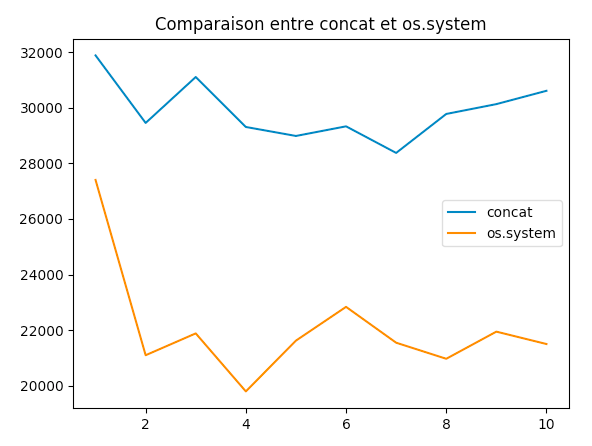
\includegraphics[width=10cm]{comparaison_concat.png}

Notons que les temps moyens d'exécution du programme complet de CRISPRbuilder\_TB pour différents systèmes d'exploitation sont relevés dans la rubrique \textit{Les tests de configuration}.




% PARALLEL FASTQ DUMP ----------------
\subsection{parallel-fastq-dump}

CRISPRbuilder\_TB utilise le module Python \textit{fastq-dump} de téléchargement et traitement de données provenant du NCBI.

\textit{fastq-dump} est un module archaïque permettant de télécharger des données relatives à un SRA dans un format \textit{.fastq} ou \textit{.fasta}. Il est contenu dans le \textit{SRA Toolkit} du NCBI. Il peut s'avérer très lent en fonction de l'utilisation en temps réel du serveur de la base de données NCBI. 

L'utilisation de plusieurs threads devrait permettre de diviser le travail en différentes tâches effectuées simultanément, et donc de gagner du temps. Malheureusement, Python n'accepte pas nativement le travail multi-threads, ce qui ne permet pas de tirer profit de systèmes multi-coeurs. C'est en fait une caractéristique de CPython. Le GIL\footnote{\index{GIL}\textbf{GIL:} Global Interpreter Lock} est un mutex qui n'autorise le travail que d'un unique thread à la fois. Il protège l'accès aux objets Python, pour empêcher de multiples threads d'exécuter du code Python simultanément. Ce verrou est rendu nécessaire parce que la gestion de la mémoire sous CPython n'est pas thread-safe. Le module \textit{parallel-fastq-dump} résout partiellement ce problème de multi-threading et utilise l'implémentation CPython en incorporant du langage C dans son contenu. Il semble être à l'heure actuelle un bon compromis gratuit pour optimiser le traitement des données vers un format \textit{.fastq} ou \textit{.fasta}. 

CRISPRbuilder\_TB utilise le module \textit{parallel-fastq-dump} pour télécharger les données d'un SRA au format \textit{.fasta}.

Notons que le \textit{SRA Tookit} est installé automatiquement au moment de l'installation de \textit{parallel-fastq-dump}.



REAL PYTHON ABOUT PYTHON THREADING




% BLAST -------------
\subsection{blast+}

CRISPRbuilder\_TB utilise également le module Python de téléchargement et traitement de données provenant du NCBI \textit{blast}.

\textit{blast} permet de trouver des régions similaires entre plusieurs séquences génomiques.  Il compare des séquences de nucléotides ou de protéines à des séquences déjà présentes dans la base de données NCBI, puis calcule la signification statistique. Il traite donc une quantité importante de données et ralentit de façon significative l'exécution du programme. \textit{blast} propose différents outils et existe sous plusieurs formes \textit{blastx, tblastn, blastn, Primer-blast, smartblast, igblast, moleblast, ...}.

Notre package effectue des comparaisons entre nucléotides. Il utilise \textit{blastn} et l'outil \texttt{makeblastdb} qui appartient à \textit{blast}. 

Les performances de \textit{blast} sont optimisées avec la suite \textit{blast+} qui utilise le \textit{Toolkit C++} du NCBI. Par ailleurs, \textit{blastn} utilise plusieurs threads pour le traitement des données et améliore encore la vitesse d'exécution de \textit{blast+}. On constate ainsi 12 threads dans le code du module \textbf{\_\_main\_\_.py}

\begin{verbatim}
  completed = subprocess.run("blastn -num_threads 12 -query " + p_spoligo_old + 
  " -evalue 1e-6 -task blastn -db " + repitem + " -outfmt '10 qseqid sseqid sstart 
  send qlen length score evalue' -out " + p_old_blast, shell=True, check=True)
\end{verbatim}







% LES TESTS DE CONFIGURATION --------------------------------
\section{Les tests de configuration}

Les tests de configuration cherchent à évaluer l'impact des différents systèmes d'exploitations et environnements matériels sur le fonctionnement d'une application.

Nous cherchons donc à définir la configuration matériele minimale afin que le package fonctionne correctement, ainsi que l'utilisabilité des différents systèmes d'exploitation.

TODO - CONFIG MINI






% CONCLUSION ----------------------
\chapter{Conclusion}

Ce stage m'a ouvert l'esprit vers le domaine de la bio-informatique, domaine intéressant qui a constitué un support scientifique très concret, me permettant de développer des compétences pratiques dans les domaines du développement et du test. 

Bien que, a priori peu attiré par le travail de validation et de test de logiciels, j'ai pu me rendre compte rapidement de son importance et en apprécier l'efficacité, vu que les tests étaient omniprésents tout au long du stage.   

Le temps passé à réfléchir aux nombreux dysfonctionnements de l'application, la frustration de comprendre tardivement que la solution provenait parfois d'éléments indépendants au code tels que l'environnement de développement ou la configuration de la variable \$PATH, le souhait de bien comprendre les rouages d'un package Python ont fortement contribué à l'amélioration de mes connaissances en informatique. 

En particulier, ce stage a mis l'accent sur les trois domaines suivants :
\begin{itemize}
\item la création d'un package Python et la gestion des dépendances,
\item la nécessité d'un campagne de tests et de validation du code,
\item la connaissance de notions clés concernant le séquençage du génome. 
\end{itemize}

Ce package fournit des informations pratiques et utiles concernant des références de SRA. Il est amené à évoluer dans l'avenir, afin de propoer une reconstitution du CRISPR dans le cadre particulier de la tubercolose.

	



????
pickle permet aux objets d'être sérialisés en fichiers sur disque et désérialisés dans le programme au moment de l'exécution.
??????
	


% INDEX ------------------
\printindex



% =========
% BIBLIOTHEQUE
% =========
\begin{spacing}{0.5}
\bibliographystyle{}
\renewcommand{\bibname}{Références}
\begin{thebibliography}{10}

\bibitem{guyeux1}Guyeux C, Sola C, Noûs C, Refrégier G. \textit{CRISPRbuilder-TB:
"CRISPR-Builder for tuberculosis''. Exhaustive reconstruction of the
CRISPR locus in Mycobacterium tuberculosis complex using SRA}. PLoS
computational biology. 2020;submitted(PCOMPBIOL-S-20-00832-2)\\ \\

\bibitem{guyeux2}Guyeux C, Sola C, Refrégier G. \textit{Exhaustive reconstruction of the
CRISPR locus in M. tuberculosis complex using short reads BioRxiv}.
2019a. doi: https://doi.org/10.1101/844746\\ \\

 \bibitem{coll-preston}Coll F, Preston M, Guerra-Assuncao JA, Hill-Cawthorn G, Harris D,
Perdigao J, et al. \textit{PolyTB: A genomic variation map for Mycobacterium
tuberculosis. Tuberculosis} (Edinb). 2014;94(3):346-54(3):346-54. doi:
10.1016/j.tube.2014.02.005. PubMed PMID: 24637013\\ \\

\bibitem{stucki-brites}Stucki D, Brites D, Jeljeli L, Coscolla M, Liu Q, Trauner A, et al.
\textit{Mycobacterium tuberculosis lineage 4 comprises globally distributed and
geographically restricted sublineages}. Nature genetics.
2016;48(12):1535-43. doi: 10.1038/ng.3704. PubMed PMID: 27798628\\ \\

\bibitem{pali-ajaw}Palittapongarnpim P, Ajawatanawong P, Viratyosin W, Smittipat N,
Disratthakit A, Mahasirimongkol S, et al. \textit{Evidence for Host-Bacterial
Co-evolution via Genome Sequence Analysis of 480 Thai Mycobacterium
tuberculosis Lineage 1 Isolates}. Scientific reports. 2018;8(1):11597.
Epub 2018/08/04. doi: 10.1038/s41598-018-29986-3. PubMed PMID: 30072734;
PubMed Central PMCID: PMCPMC6072702\\ \\

\bibitem{shiti-kolchenko}Shitikov E, Kolchenko S, Mokrousov I, Bespyatykh J, Ischenko D, Ilina E, et al. \textit{Evolutionary pathway analysis and unified classification of
East Asian lineage of Mycobacterium tuberculosis}. Scientific reports.
2017;7(1):9227. doi: 10.1038/s41598-017-10018-5. PubMed PMID: 28835627;
PubMed Central PMCID: PMCPMC5569047\\ \\

\bibitem{kamerbeek-schouls}Kamerbeek J, Schouls L, Kolk A, van Agterveld M, van Soolingen D, Kuijper S, et al. \textit{Simultaneous detection and strain differentiation of
Mycobacterium tuberculosis for diagnosis and epidemiology}. J Clin
Microbiol. 1997;35(4):907-14. PubMed PMID: 9157152\\ \\

\bibitem{embden}van Embden JDA, van Gorkom T, Kremer K, Jansen R, van der Zeijst BAM,
Schouls LM. \textit{Genetic variation and evolutionary origin of the Direct
repeat locus of Mycobacterium tuberculosis complex bacteria}, J
Bacteriol. 2000;182:2393-401\\ \\

\bibitem{comas}Comas I. et al. \textit{Out-of-Africa migration and Neolithic coexpansion of Mycobacterium tuberculosis with modern humans}, Nat Genet. 45(10): 1176–1182. doi:10.1038/ng.2744\\ \\

\bibitem{coll}Coll F. et al., \textit{SpolPred : rapid and accurate prediction of Mycobacterium tuberculosis spoligotypes from short genomic sequences}, Bioinformatics. 28(22):2991–3\\ \\

\bibitem{brynildsrud}Brynildsrud O.B. et al., \textit{Global expansion of Mycobacterium tuberculosis lineage 4 shaped by colonial migration and local adaptation}, 4(10): eaat5869. doi: 10.1126/sciadv.aat5869\\ \\

\bibitem{driscoll}Driscoll J. R., \textit{Spoligotyping for molecular epidemiology of the Mycobacterium tuberculosis complex}, 551:117-28. doi: 10.1007/978-1-60327-999-4 10\\ \\

\bibitem{jinek}Jinek M. et al, \textit{A programmable dual-RNA-guided DNA endonuclease in adaptive bacterial immunity}, 337(6096):816-21. doi: 10.1126/science.1225829\\ \\

\bibitem{gori}Gori A. et al, \textit{Spoligotyping and Mycobacterium tuberculosis}, 11(8): 1242–1248. doi: 10.3201/1108.040982\\ \\

\bibitem{perry1}Perry S. et al., \textit{Infection with Helicobacter pylori is associated with protection against tuberculosis}, 5(1):e8804. doi: 10.1371/journal.pone.0008804\\ \\

\bibitem{perry2}Perry S. et al, \textit{The immune response to tuberculosis infection in the setting of Helicobacter pylori and helminth infections}, 141(6): 1232–1243. doi: 10.1017/S0950268812001823\\ \\

\bibitem{xia}Xia E. et al., \textit{SpoTyping: fast and accurate in silico Mycobacterium spoligotyping from sequence reads}, 8:19. doi 10.1186/s13073-016-0270-7\\ \\ 

\bibitem{dale}Dale JW. et al., \textit{Spacer oligonucleotide typing of bacteria of the Mycobacterium tuberculosis complex: recommendations for standardised nomenclature.}, 5(3):216–9\\ \\

\bibitem{iwai}Iwai H et al., \textit{CASTB (the comprehensive analysis server for the Mycobacterium tuberculosis complex): A publicly accessible web server for epidemiological analyses, drug-resistance prediction and phylogenetic comparison of clinical isolates. Tuberculosis.}, 95(6):843–4\\ \\

\bibitem{demay}Demay C. et al., \textit{SITVITWEB - A publicly available international multimarker database for studying Mycobacterium tuberculosis genetic diversity and molecular epidemiology.}, Infect Genet Evol. 12:755–66\\ \\

\bibitem{}McGovern Institute Channel, \textit{Genome Editing with CRISPR-Cas9}, \url{https://www.youtube.com/watch?v=2pp17E4E-O8}\\ \\

\bibitem{oneil}O'Neil M.B. et al., \textit{Lineage specific histories of Mycobacterium tuberculosis dispersal in Africa and Eurasia}, bioRxiv. 10.1101/210161\\ \\

\bibitem{ratovonirina}Ratovonirina N. H., \textit{Etudes descriptive, épidémiologique, moléculaire et spatiale des souches Mycobacterium tuberculosis circulant à Antananarivo, Madagascar}, Thèse de Doctorat de l'Université Paris-Saclay\\ \\

\bibitem{kamerbeek}Kamerbeek et al., \textit{Simultaneous detection and strain differentiation of Mycobacterium tuberculosis for diagnosis and epidemiology}, 35(4): 907–914\\ \\

\bibitem{mendis}Mendis C. et al., \textit{Insight into genetic diversity of Mycobacterium tuberculosis in Kandy, Sri Lanka reveals predominance of the Euro-American lineage}, International Journal of Infectious Diseases 87 84-91\\ \\

\bibitem{gomgnimbou},Gomgnimbou M. K. et al., \textit{Tuberculosis-Spoligo-Rifampin-Isoniazid Typing: an All-in-One Assay Technique for Surveillance and Control of Multidrug-Resistant Tuberculosis on Luminex Devices}, 51(11):3527-34. doi: 10.1128/JCM.01523-13\\ \\

\bibitem{couvin}Couvin D. et al., \textit{SpolSimilaritySearch - A web tool to compare and search similarities between spoligotypes of Mycobacterium tuberculosis complex}, 105:49-52. doi: 10.1016/j.tube.2017.04.007


\end{thebibliography}
\end{spacing}

\end{document}
